\documentclass{beamer}
\setbeamertemplate{navigation symbols}{}
\usepackage{comment}

\setbeamercolor{frametitle}{fg=black,bg=white}
\setbeamercolor{title}{fg=black,bg=yellow!85!orange}
\usetheme{AnnArbor}

\usepackage{textpos} % package for the positioning
\usepackage{listings}
\usepackage{xcolor}
\usepackage[most]{tcolorbox}
\usepackage{mathtools}
\usepackage{graphicx}
\usepackage{graphbox}
\usepackage{movie15}
\usepackage{caption}
\DeclareCaptionType{code}[Code Listing][List of Code Listings] 

\definecolor{codegreen}{rgb}{0,0.6,0}
\definecolor{codegray}{rgb}{0.5,0.5,0.5}
\definecolor{codepurple}{rgb}{0.58,0,0.82}
\definecolor{backcolour}{rgb}{0.95,0.95,0.92} 
\lstdefinestyle{mystyle}{
    backgroundcolor=\color{backcolour},   
    commentstyle=\color{codegreen},
    keywordstyle=\color{magenta},
    numberstyle=\tiny\color{codegray},
    stringstyle=\color{codepurple},
    basicstyle=\ttfamily\footnotesize,
    breakatwhitespace=false,         
    breaklines=true,                 
    captionpos=b,                    
    keepspaces=true,                 
    numbers=left,                    
    numbersep=5pt,                  
    showspaces=false,                
    showstringspaces=false,
    showtabs=false,                  
    tabsize=2
}

\lstset{style=mystyle}

\lstdefinelanguage
   [x64]{Assembler}     % add a "x64" dialect of Assembler
   [x86masm]{Assembler} % based on the "x86masm" dialect
   % with these extra keywords:
   {morekeywords={CDQE,CQO,CMPSQ,CMPXCHG16B,JRCXZ,LODSQ,MOVSXD, %
                  POPFQ,PUSHFQ,SCASQ,STOSQ,IRETQ,RDTSCP,SWAPGS, %
                  rax,rdx,rcx,rbx,rsi,rdi,rsp,rbp, %
                  r8,r8d,r8w,r8b,r9,r9d,r9w,r9b, %
                  r10,r10d,r10w,r10b,r11,r11d,r11w,r11b, %
                  r12,r12d,r12w,r12b,r13,r13d,r13w,r13b, %
                  r14,r14d,r14w,r14b,r15,r15d,r15w,r15b}} %


\beamersetuncovermixins{\opaqueness<1>{25}}{\opaqueness<2->{15}}

%Copyright
\addtobeamertemplate{frametitle}{}{%
\begin{textblock*}{50mm}(0cm,-1.25cm)
\color{yellow!85!orange}
\tiny{Copyright \copyright 2024 CNM.}
\end{textblock*}}

% position the logo
\addtobeamertemplate{frametitle}{}{%
\begin{textblock*}{100mm}(11.4cm,-1.3cm)

\includegraphics[height=1cm,width=1cm,keepaspectratio]{fig/ddclogotransparent.png}
\end{textblock*}}

\AtBeginSection[]{
  \begin{frame}
  \vfill
  \centering
  \begin{beamercolorbox}[sep=8pt,center,shadow=true,rounded=true]{title}
    \usebeamerfont{title}\insertsectionhead\par%
  \end{beamercolorbox}
  \vfill
  \end{frame}
}

\begin{document}
\title{Quantum Technician Bootcamp}
\author{Brian Rashap}
\date{September 2025} 

\begin{frame}
\titlepage
\end{frame}

\section{Introduction}

\begin{frame}\frametitle{Instructional team}
A physicist, an engineer, and a technician walk into a classroom...
\end{frame}

\begin{frame}
\frametitle{The Engineer: Brian Rashap, Ph.D.}
\begin{columns}
\begin{column}{6.5cm}
\begin{itemize}
\item Proud husband of Krista and father of Shelby (27) and Ethan (23)
\item Electrical Engineer (Michigan) with 23 years industrial experience (Intel)
\item Created and taught IoT Bootcamp for 5 years (and going)
\item Hobbies: painting, cycling, swimming, reading, spending time with family
\end{itemize}
\end{column}
\begin{column}{4.5cm}
\begin{center}
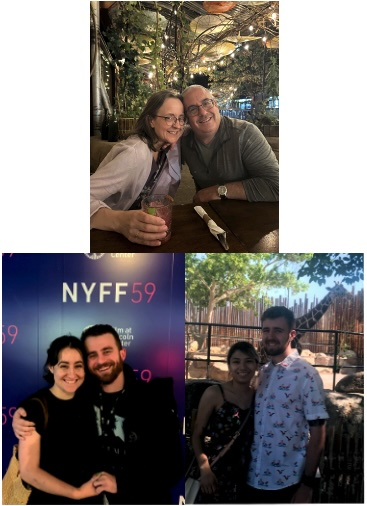
\includegraphics[width=4.5cm]{fig/rashapfamily.jpg}
\end{center}
\end{column}
\end{columns}
\end{frame}

\begin{frame}
\frametitle{The Physicist: Megan Ivory}
\begin{columns}
\begin{column}{7cm}
\begin{itemize}
\item 
\end{itemize}
\vspace{1cm} 
\end{column}
\begin{column}{4cm}
\begin{center}

\end{center}
\end{column}
\end{columns}
\end{frame}

\begin{frame}
\frametitle{The Technician: Shawn Morales}
\begin{columns}
\begin{column}{7cm}
\begin{itemize}
\item 

\vspace{0.25cm}

\end{itemize}
\vspace{1cm} 
\end{column}
\begin{column}{4cm}
\begin{center}

\end{center}
\end{column}
\end{columns}
\end{frame}








\begin{frame}\frametitle{Student Introductions}
\begin{itemize}
\item Your name
\item What were you up to before starting the bootcamp
\item Any prior experience with math, science, machining, etc.
\item What do you hope to get out of the bootcamp
\end{itemize}
\end{frame}

\begin{frame}\frametitle{Class Rules}
\begin{itemize}
\item Respect each other. Help each other.
\item Ask questions. 
\item Be on time (let us know via Slack if you won't be here) 
\item Keep your workspace and the classroom neat and tidy.
\item If you are struggling, let us know. We are here to HELP!
\item Class hours
\begin{itemize}
\item Mon-Th: 8am to 5pm \footnote{Doors open at 7:50, please be in your seats ready to learn by 8:00} and Friday: 8am to 3pm \footnote{Occasionally on Friday there will be optional activities from 3 to 5}
\item Lunch Break: 1 hour near noon. Maybe combined with work time. 
\item Please respect the instructors' lunch break as well.
\end{itemize}
\item Phone Policy: phones should not be out or used during class
\begin{itemize}
\item No gaming, no surfing social media
\item If you need to take/make a call, please set out of the classroom
\item Exceptions: two-factor authentication, pictures of projects, class videos
\end{itemize}
\end{itemize}
\end{frame}

\begin{frame}\frametitle{Important Attribute in an Employee}
\begin{itemize}
\item Tolerance of Ambiguity
\item Attention to Detail
\item Curiosity
\item Structured Problem Solving
\end{itemize}
\end{frame}


\section{Overview: QIS in NM}

\begin{frame}\frametitle{Introduction}
\begin{center}
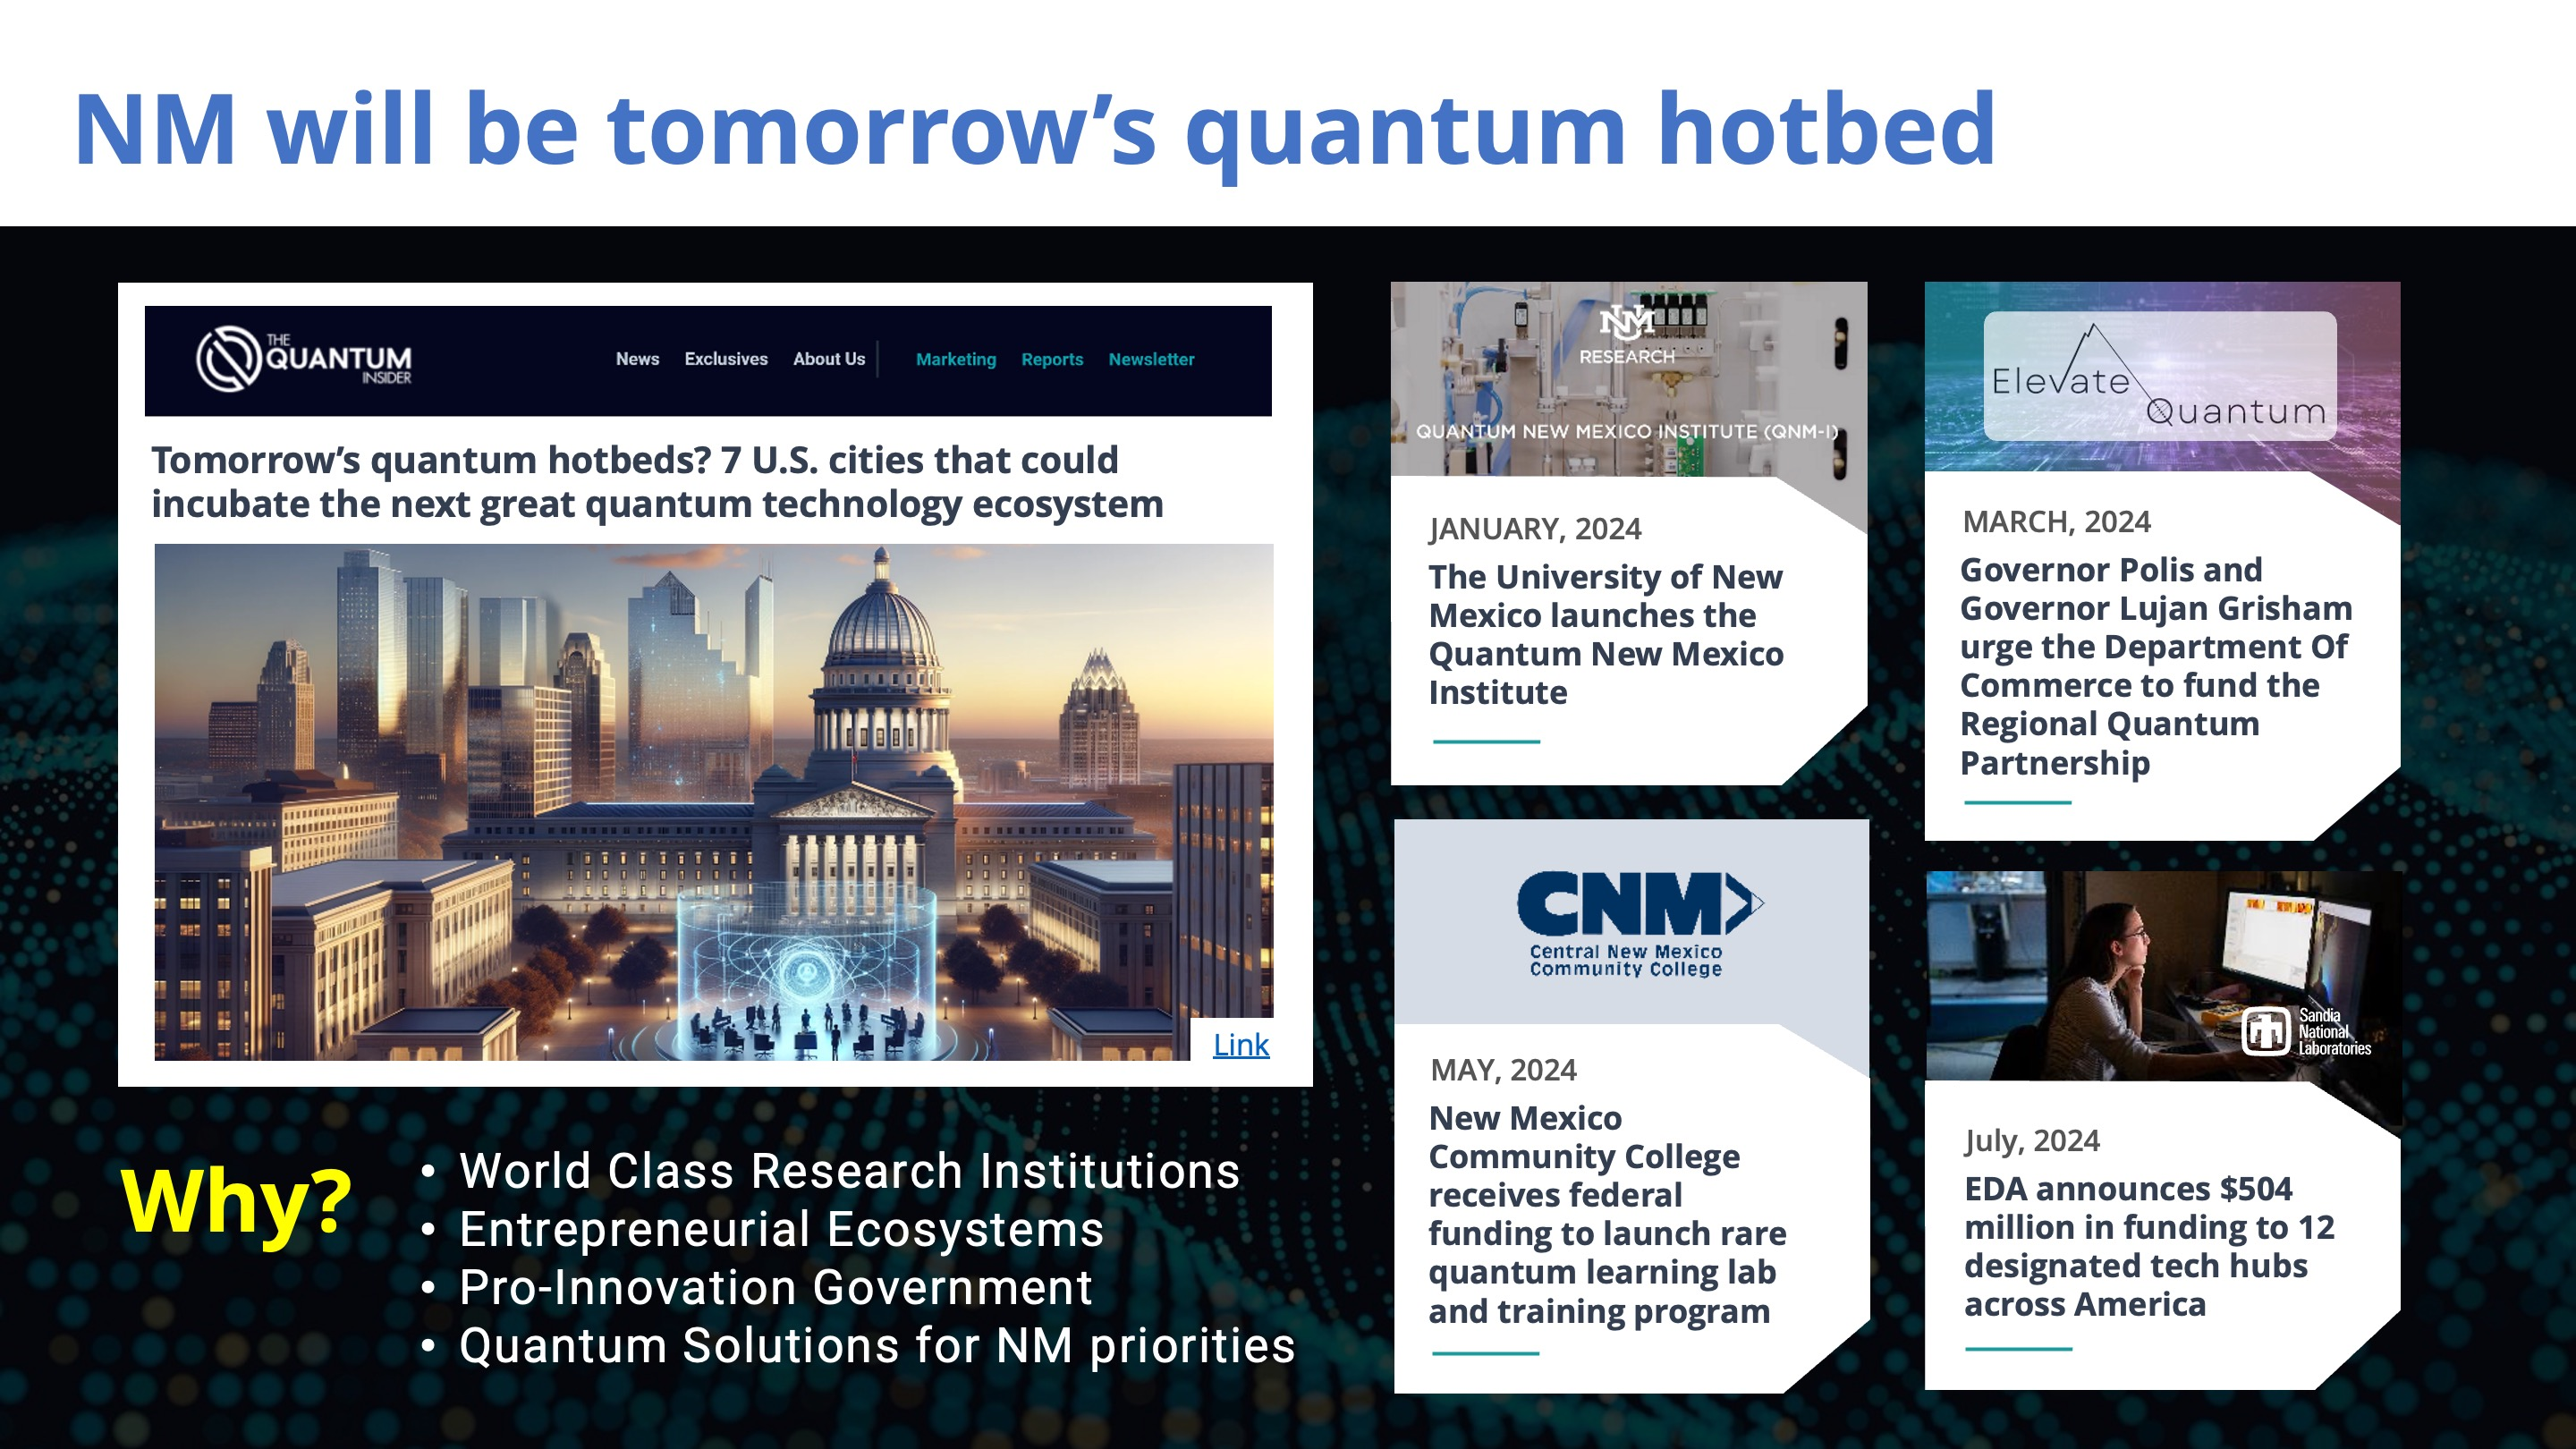
\includegraphics[width=12cm]{fig/Slide2.jpeg}
\end{center}
\end{frame}

\begin{frame}\frametitle{Introduction}
\begin{center}
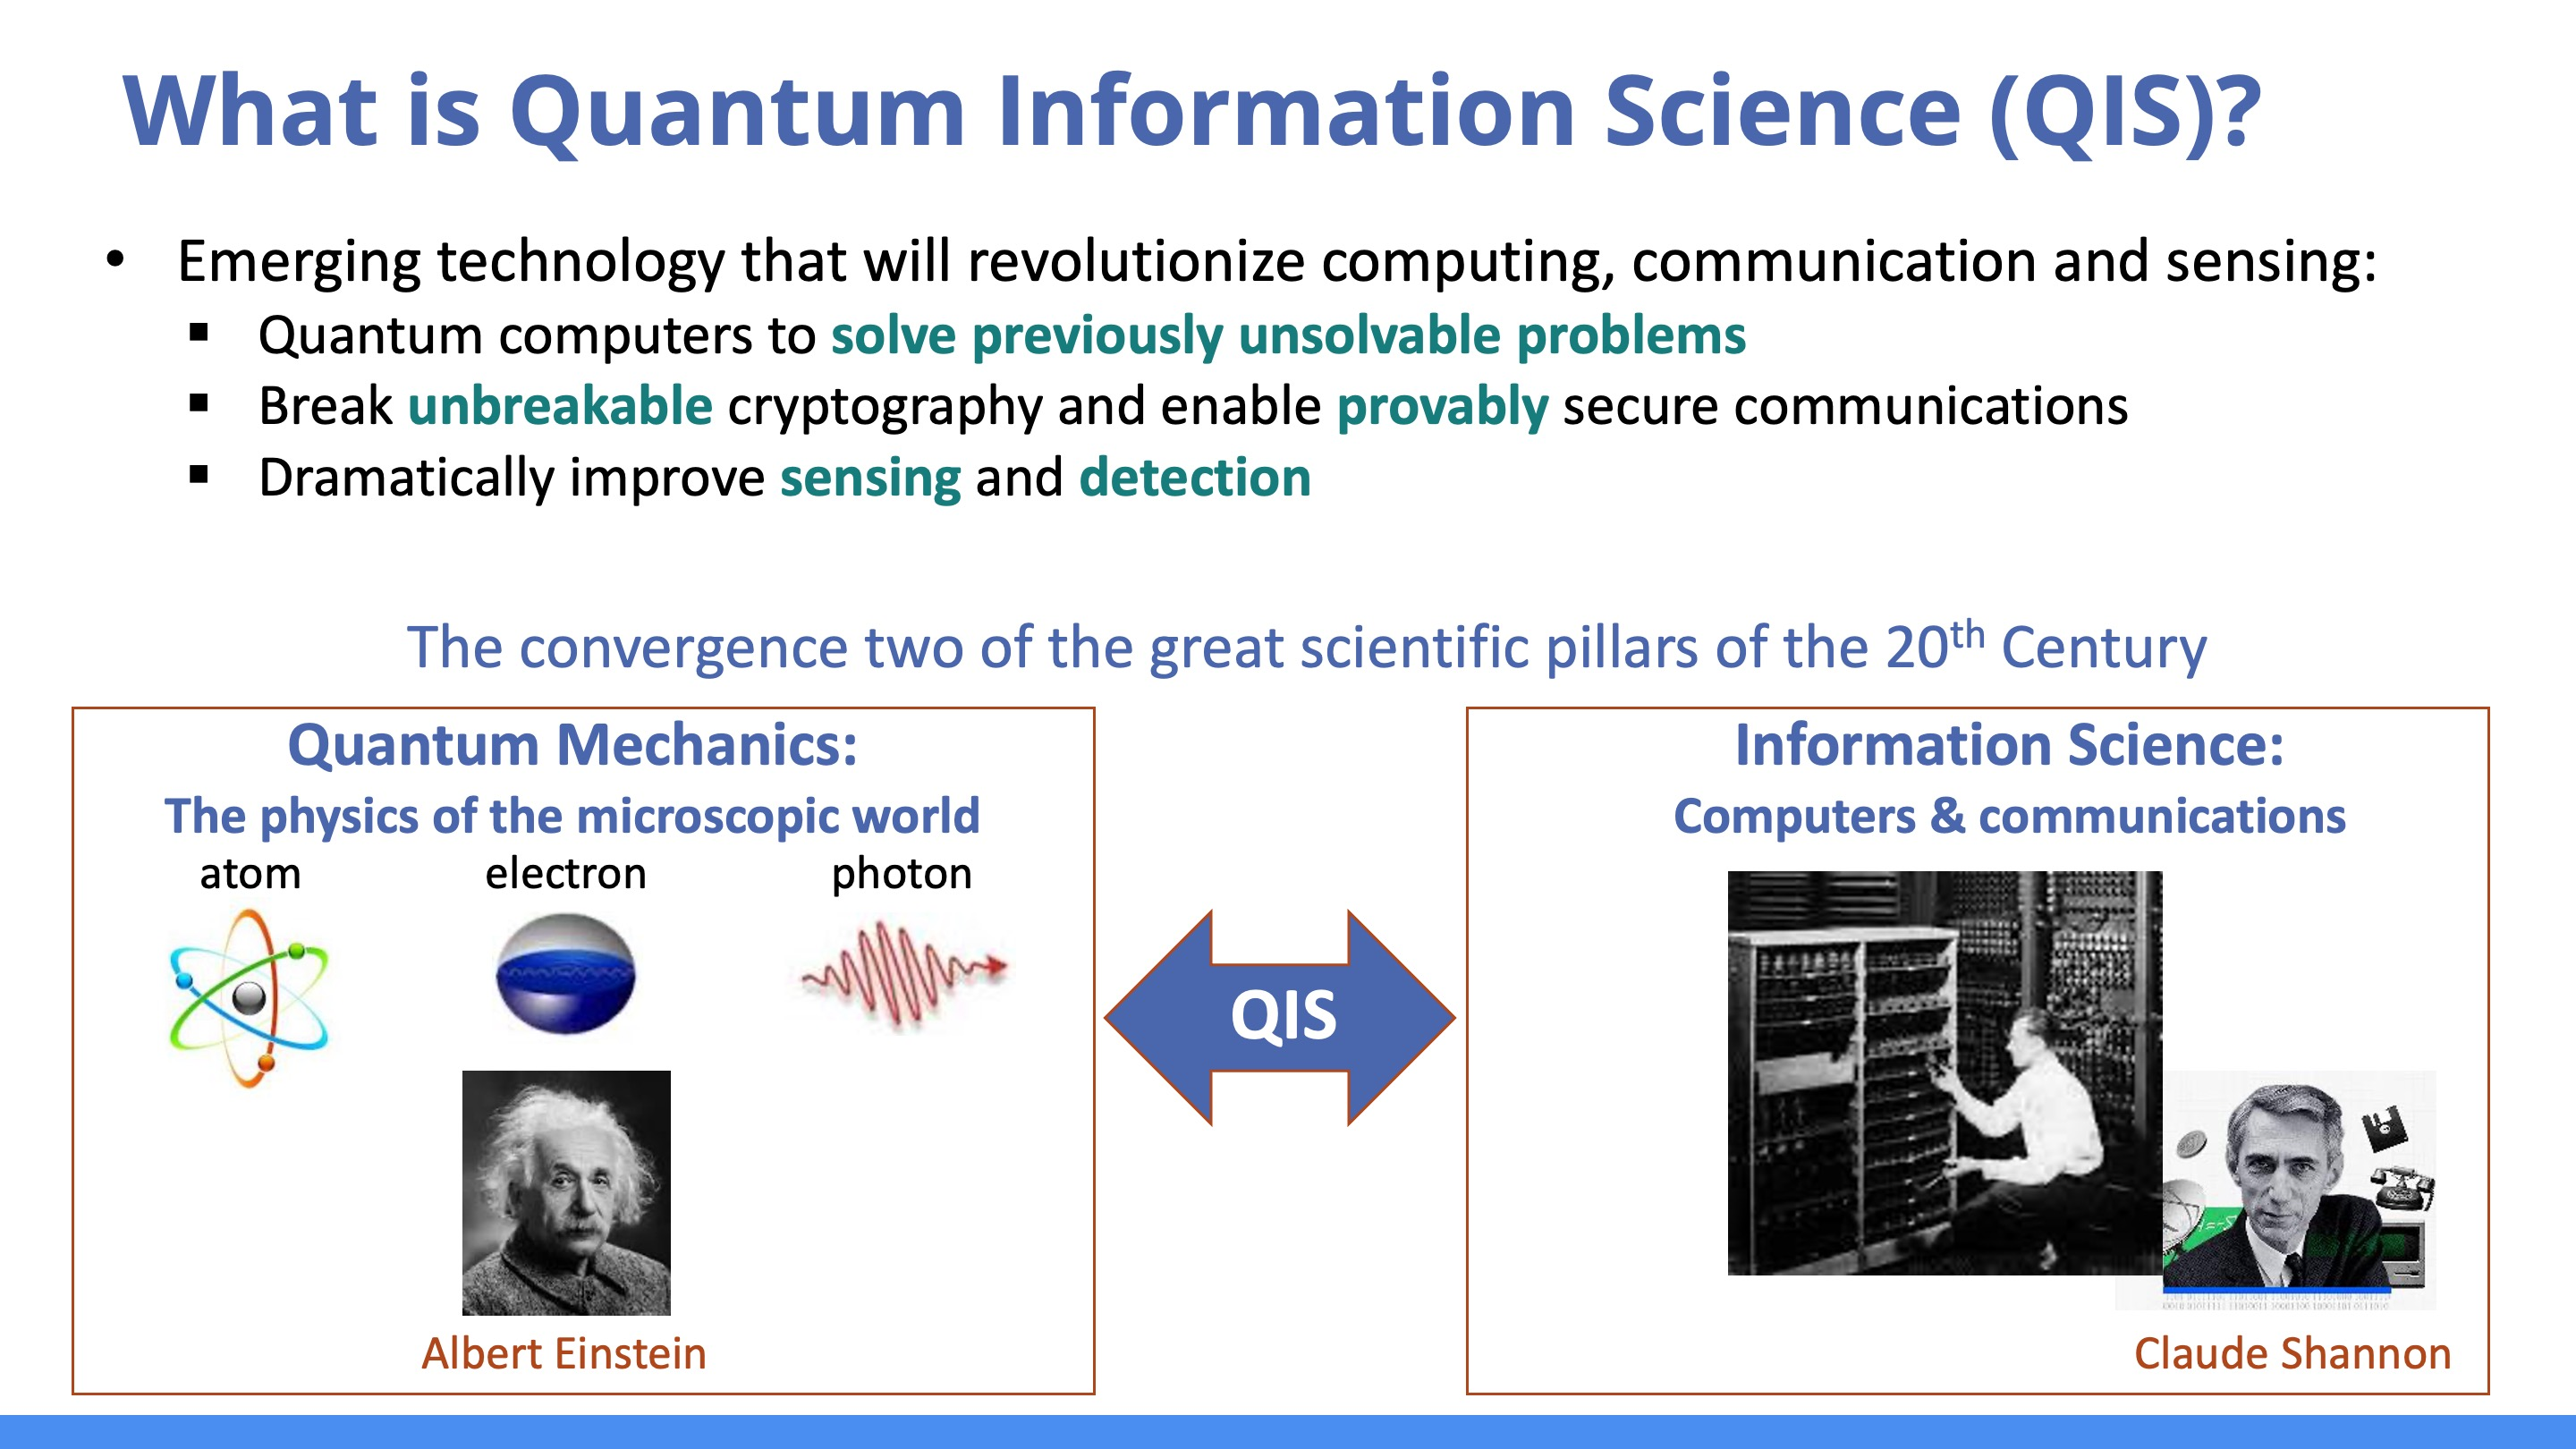
\includegraphics[width=12cm]{fig/Slide4.jpeg}
\end{center}
\end{frame}

\begin{frame}\frametitle{Introduction}
\begin{center}
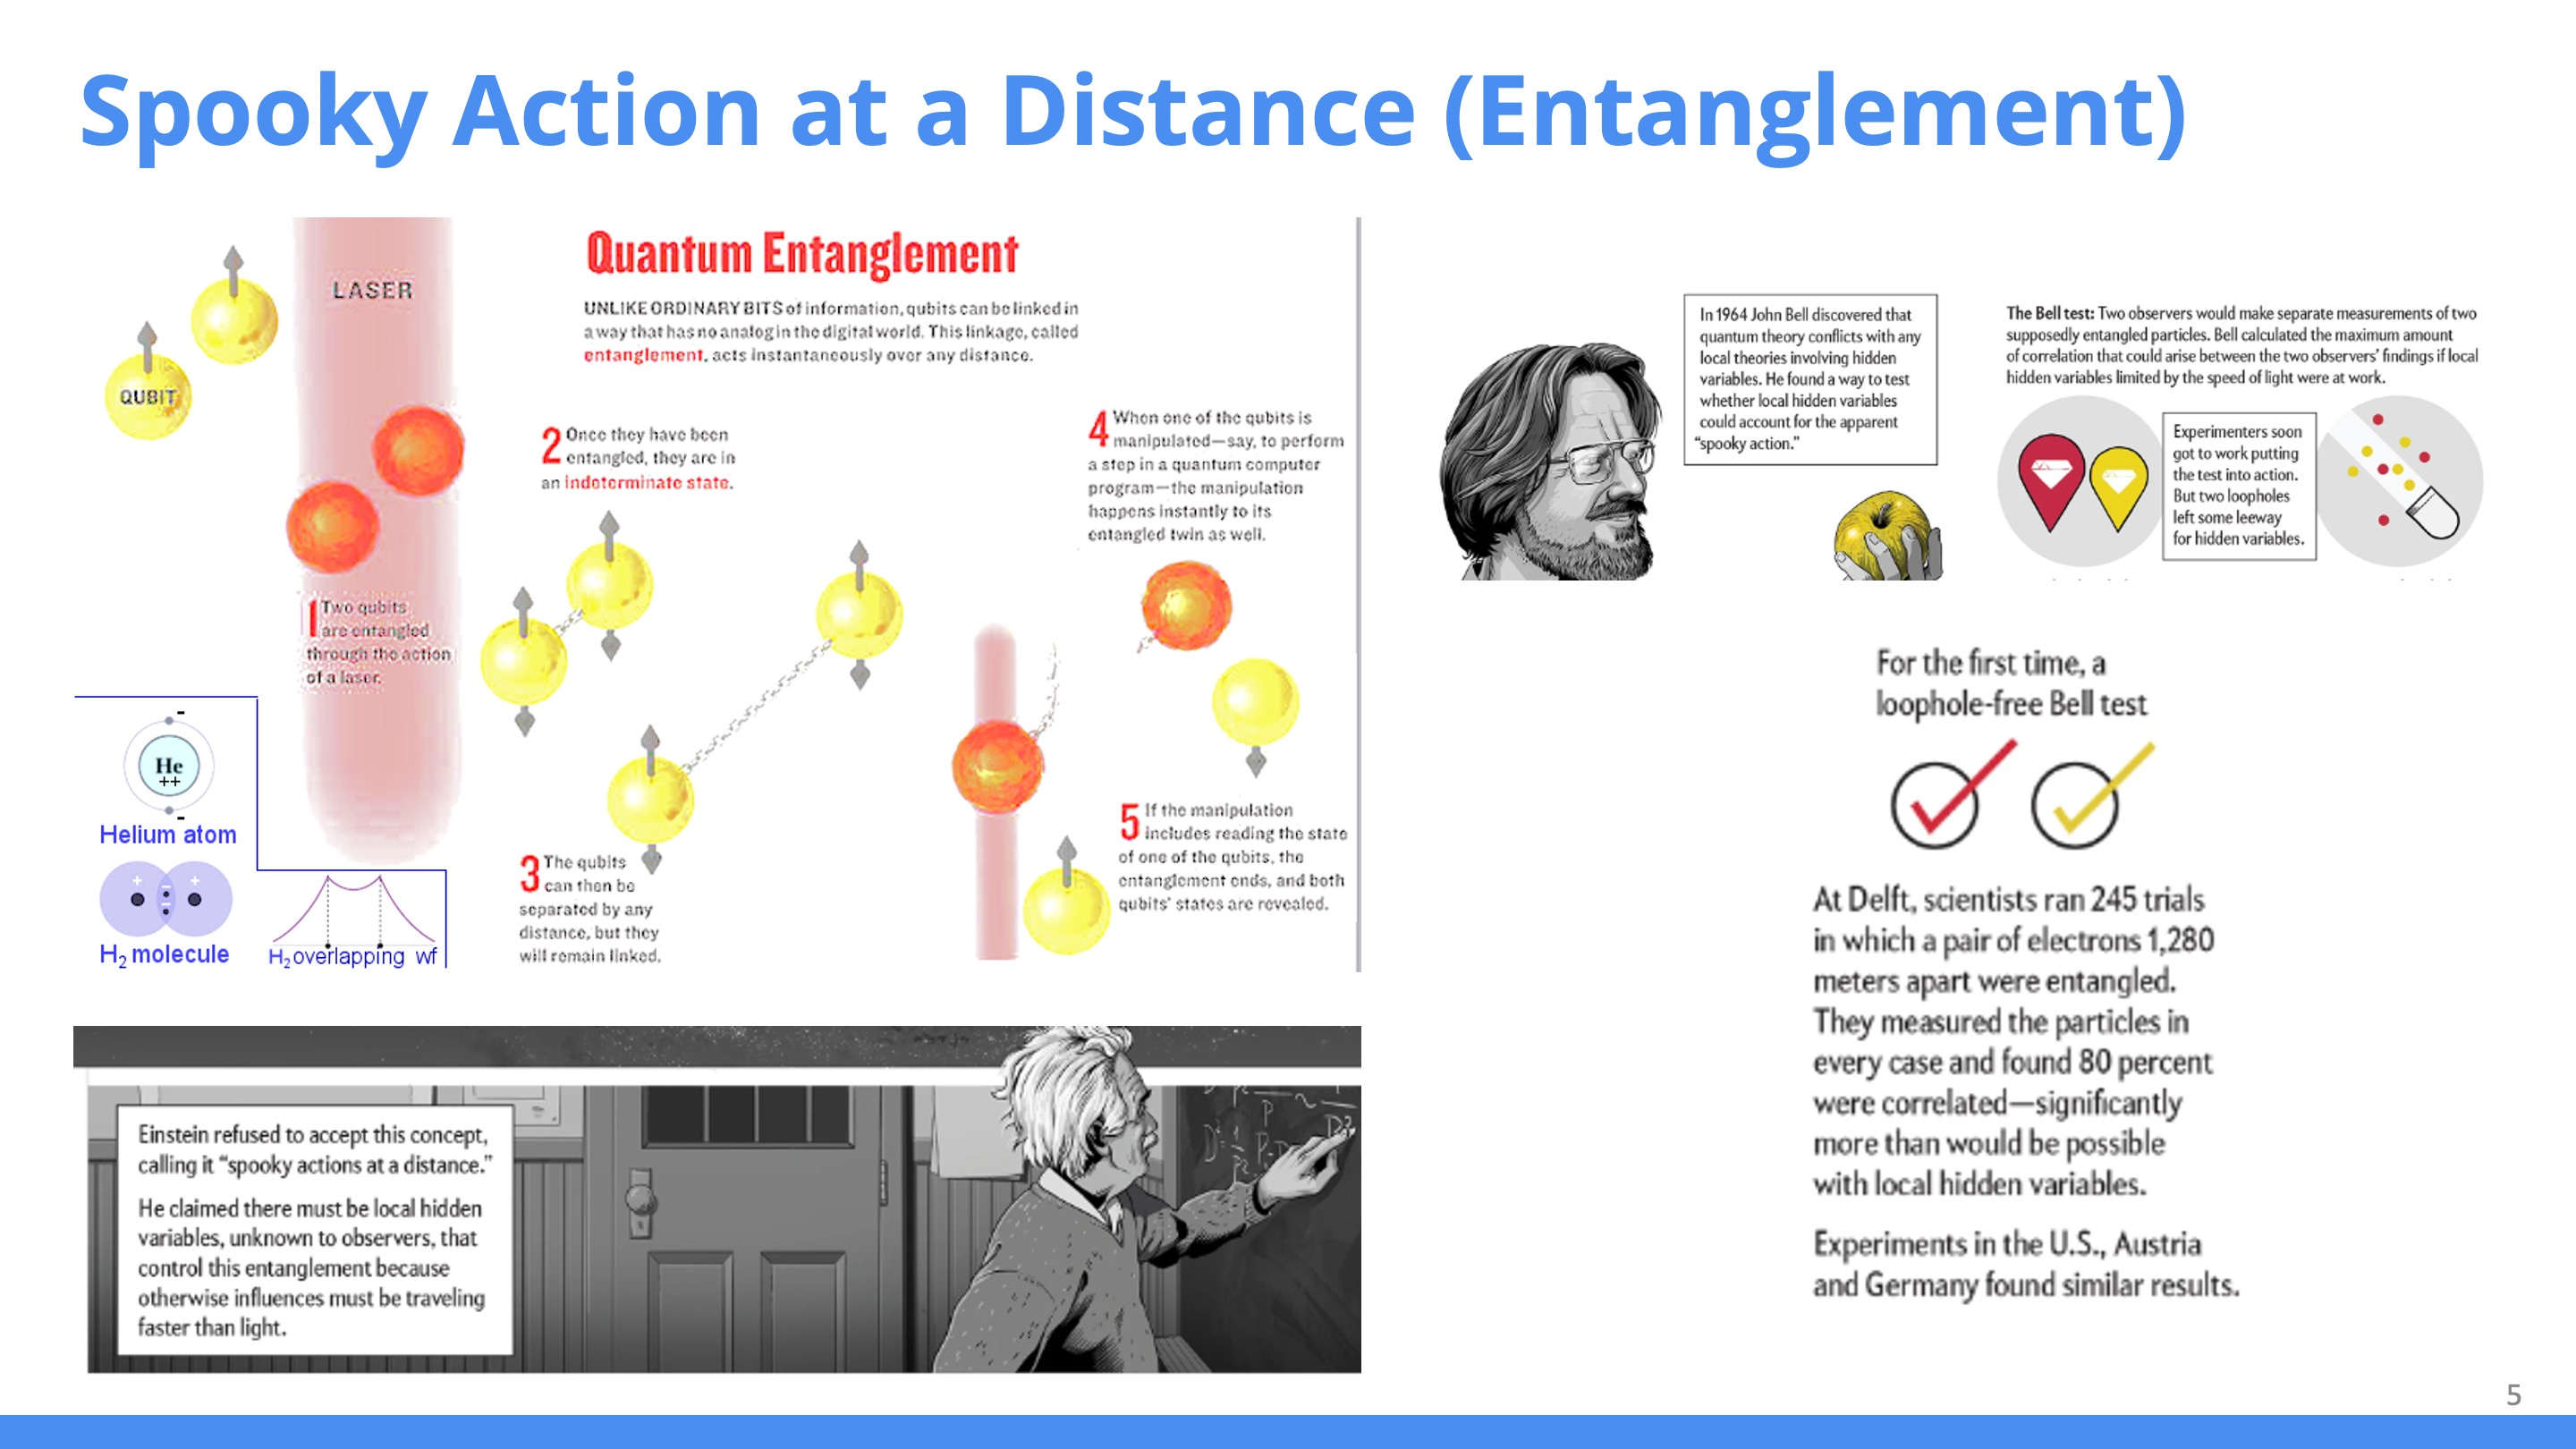
\includegraphics[width=12cm]{fig/Slide5.jpeg}
\end{center}
\end{frame}

\begin{frame}\frametitle{Introduction}
\begin{center}
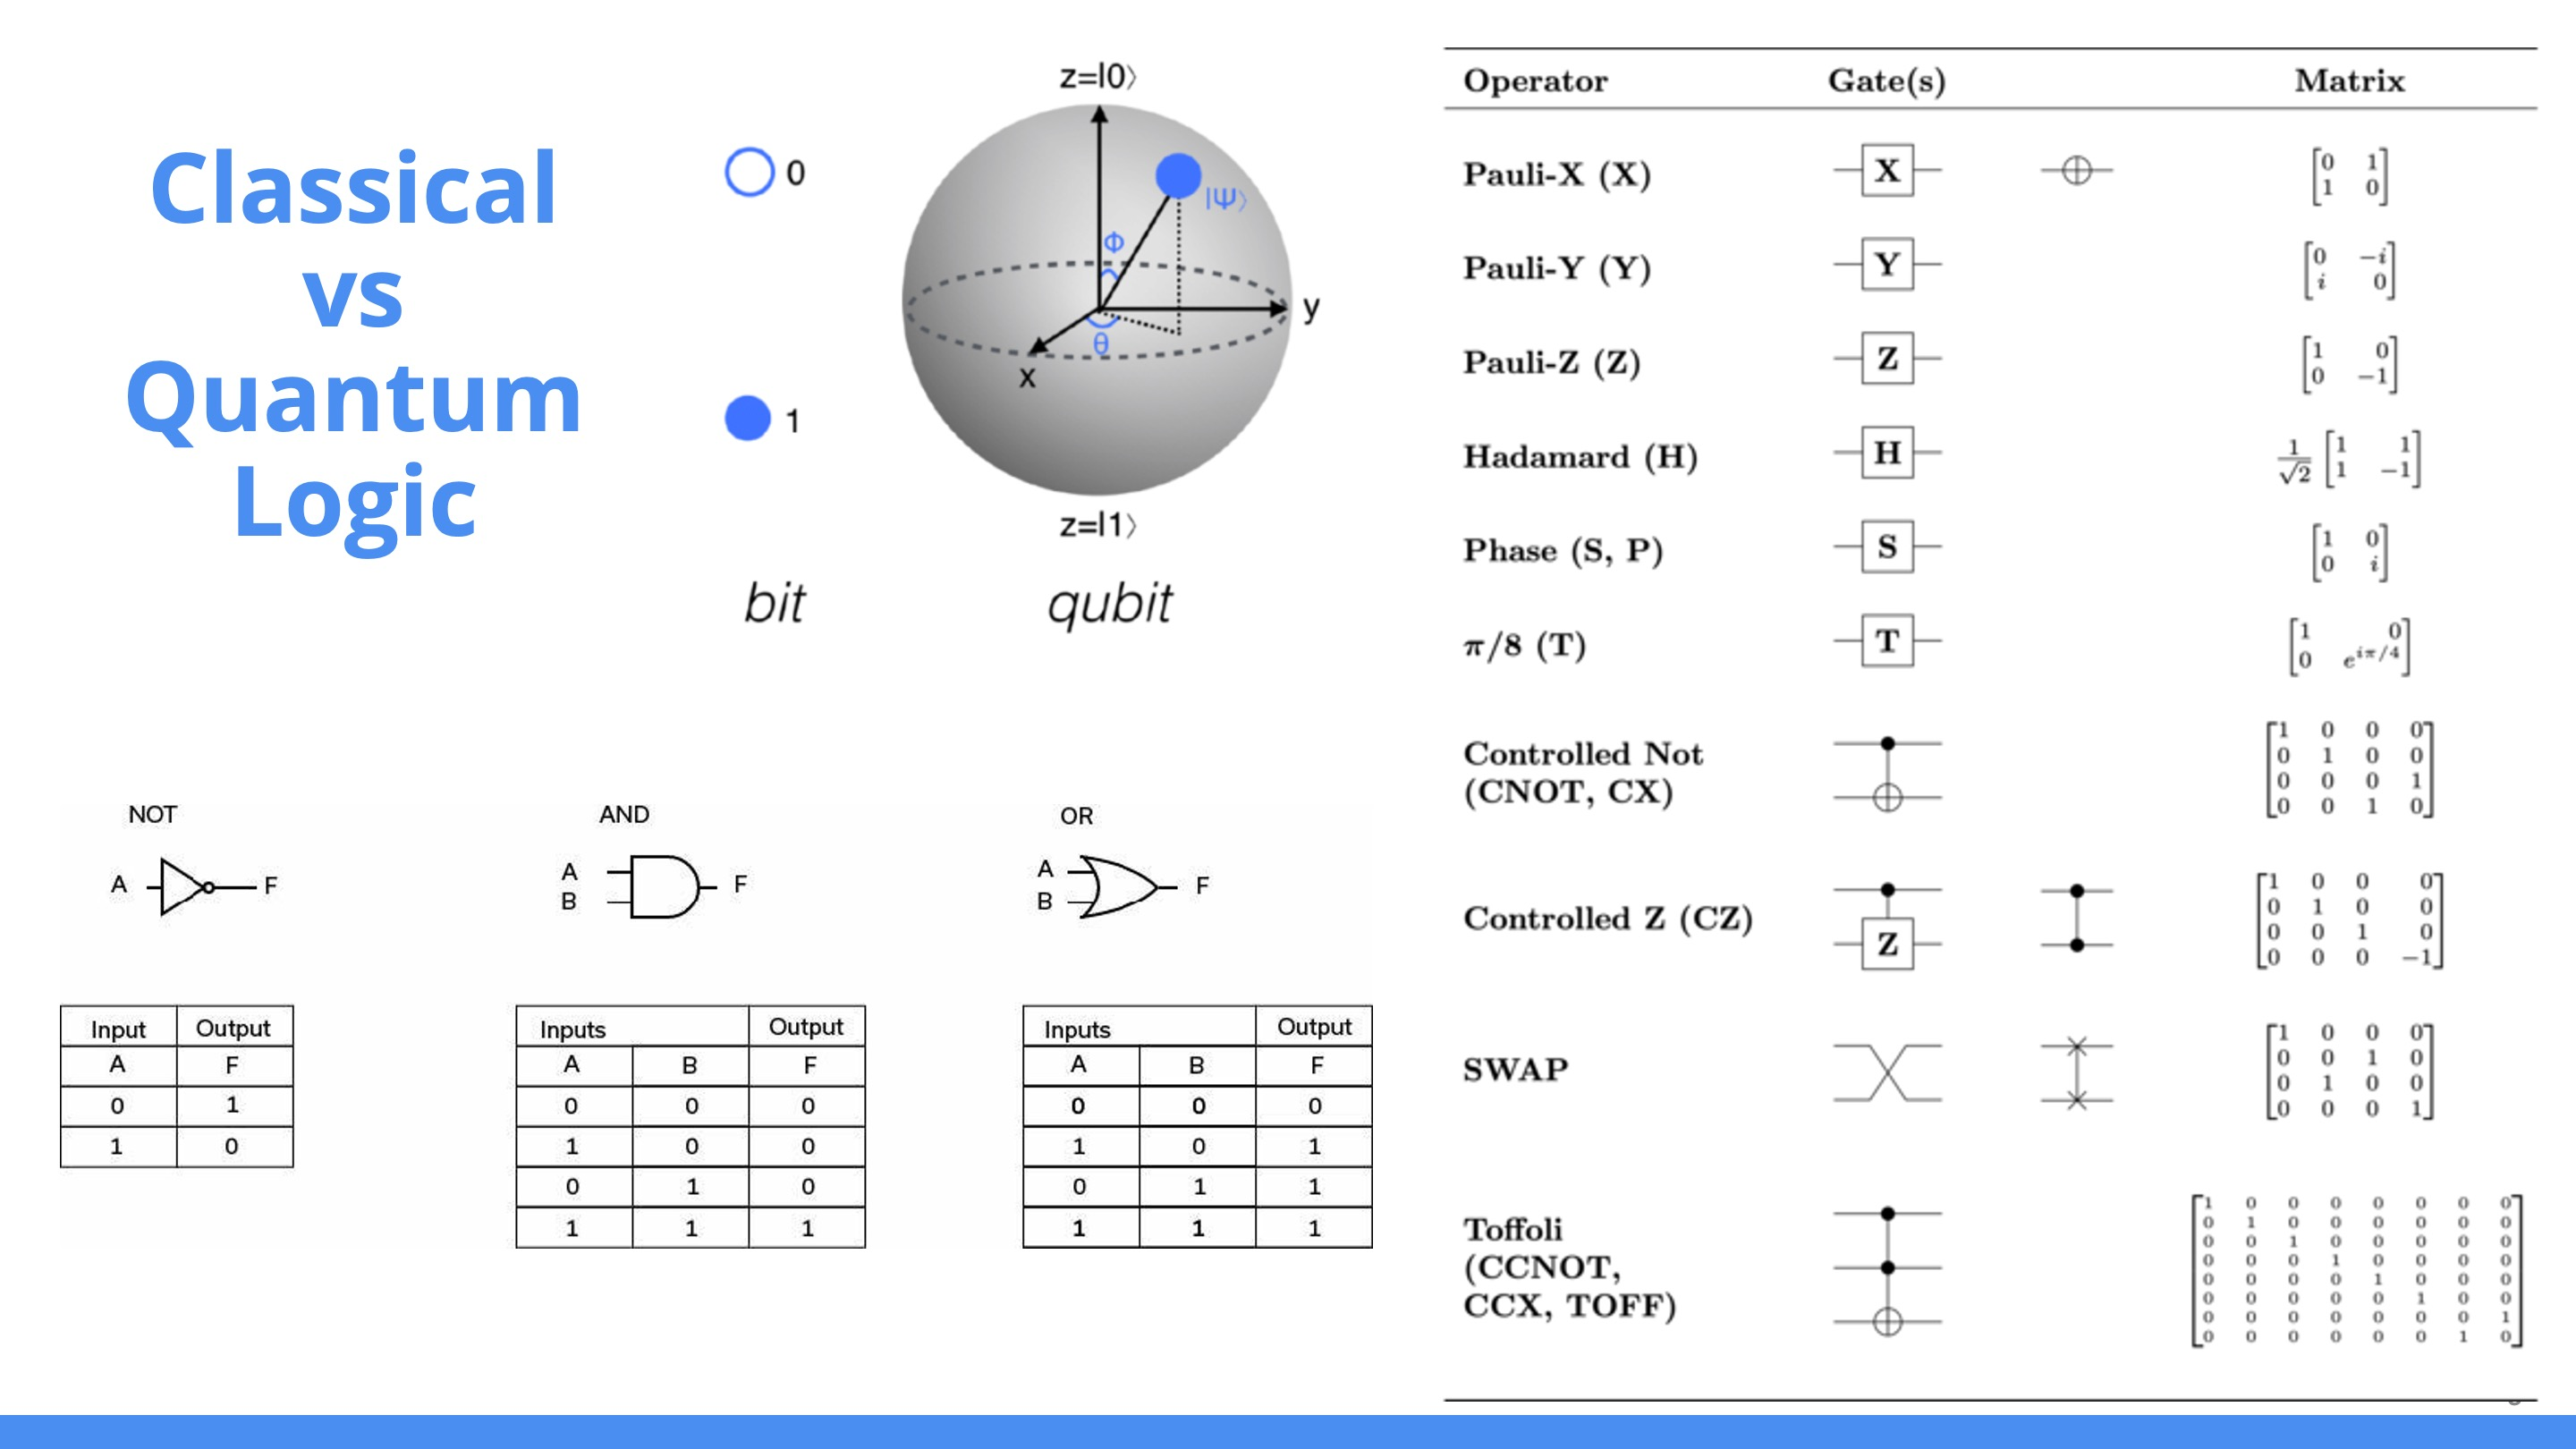
\includegraphics[width=12cm]{fig/Slide6.jpeg}
\end{center}
\end{frame}

\begin{frame}\frametitle{Introduction}
\begin{center}
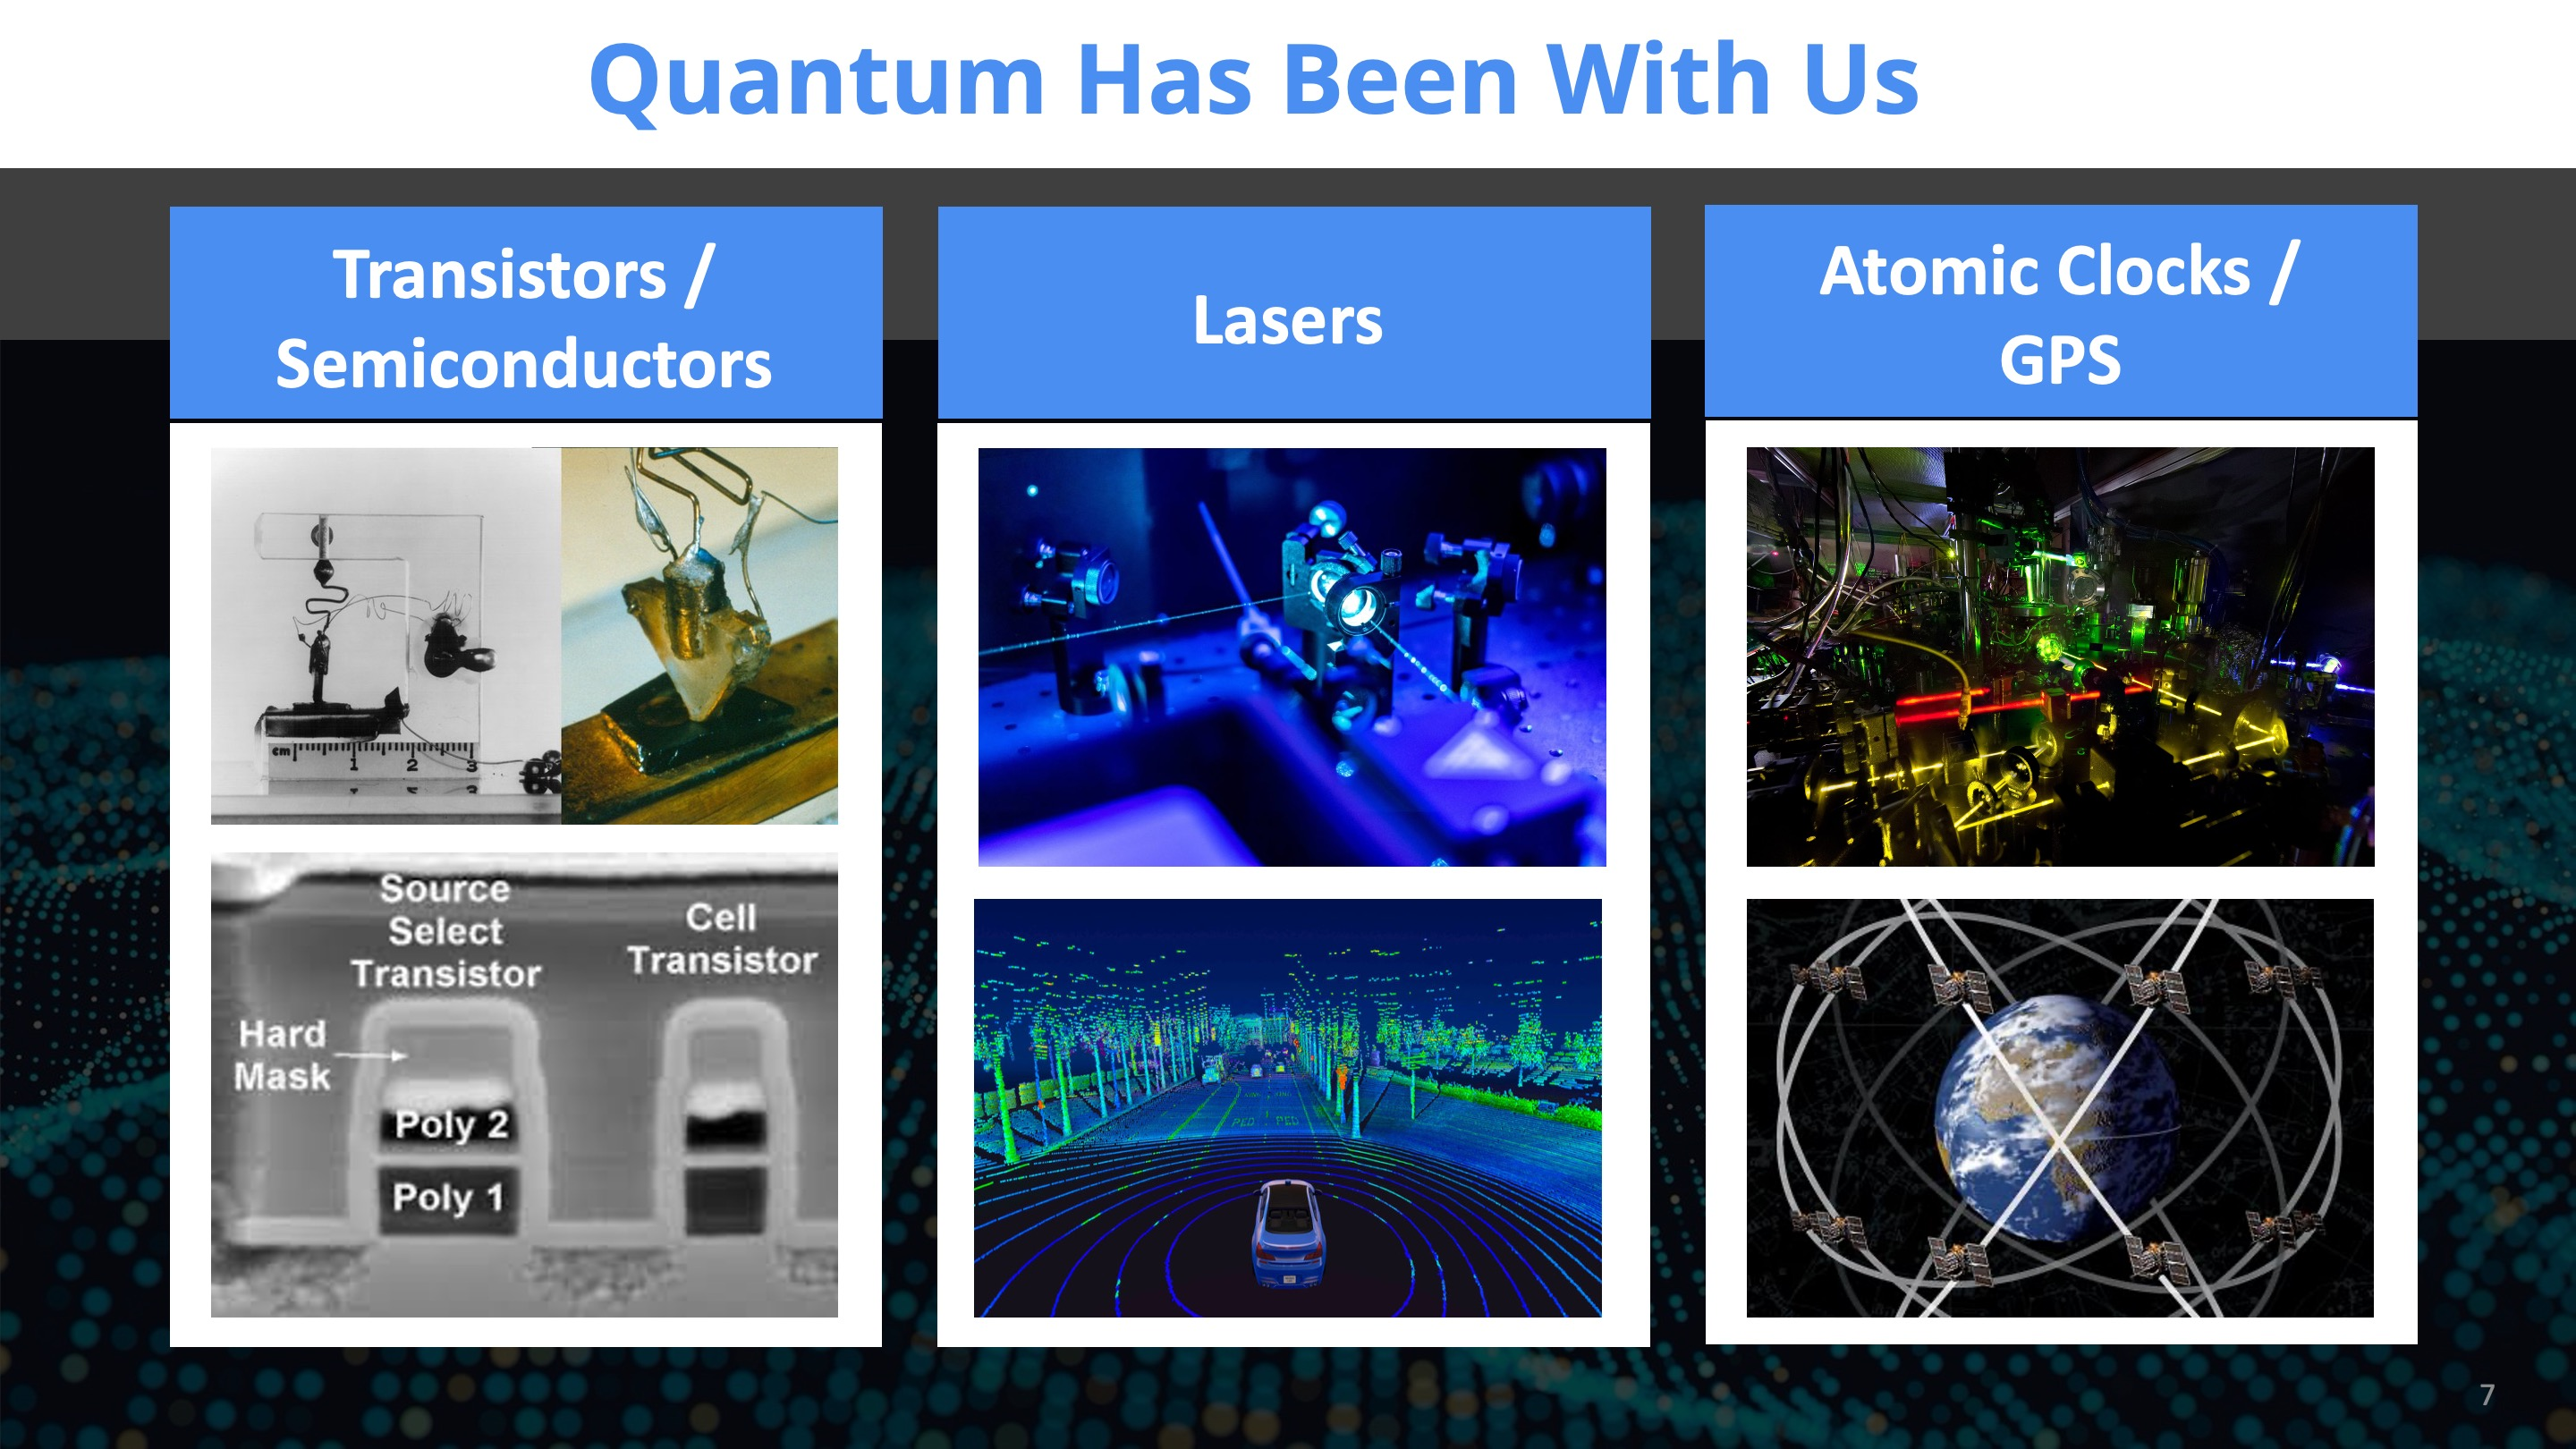
\includegraphics[width=12cm]{fig/Slide7.jpeg}
\end{center}
\end{frame}

\begin{frame}\frametitle{Introduction}
\begin{center}
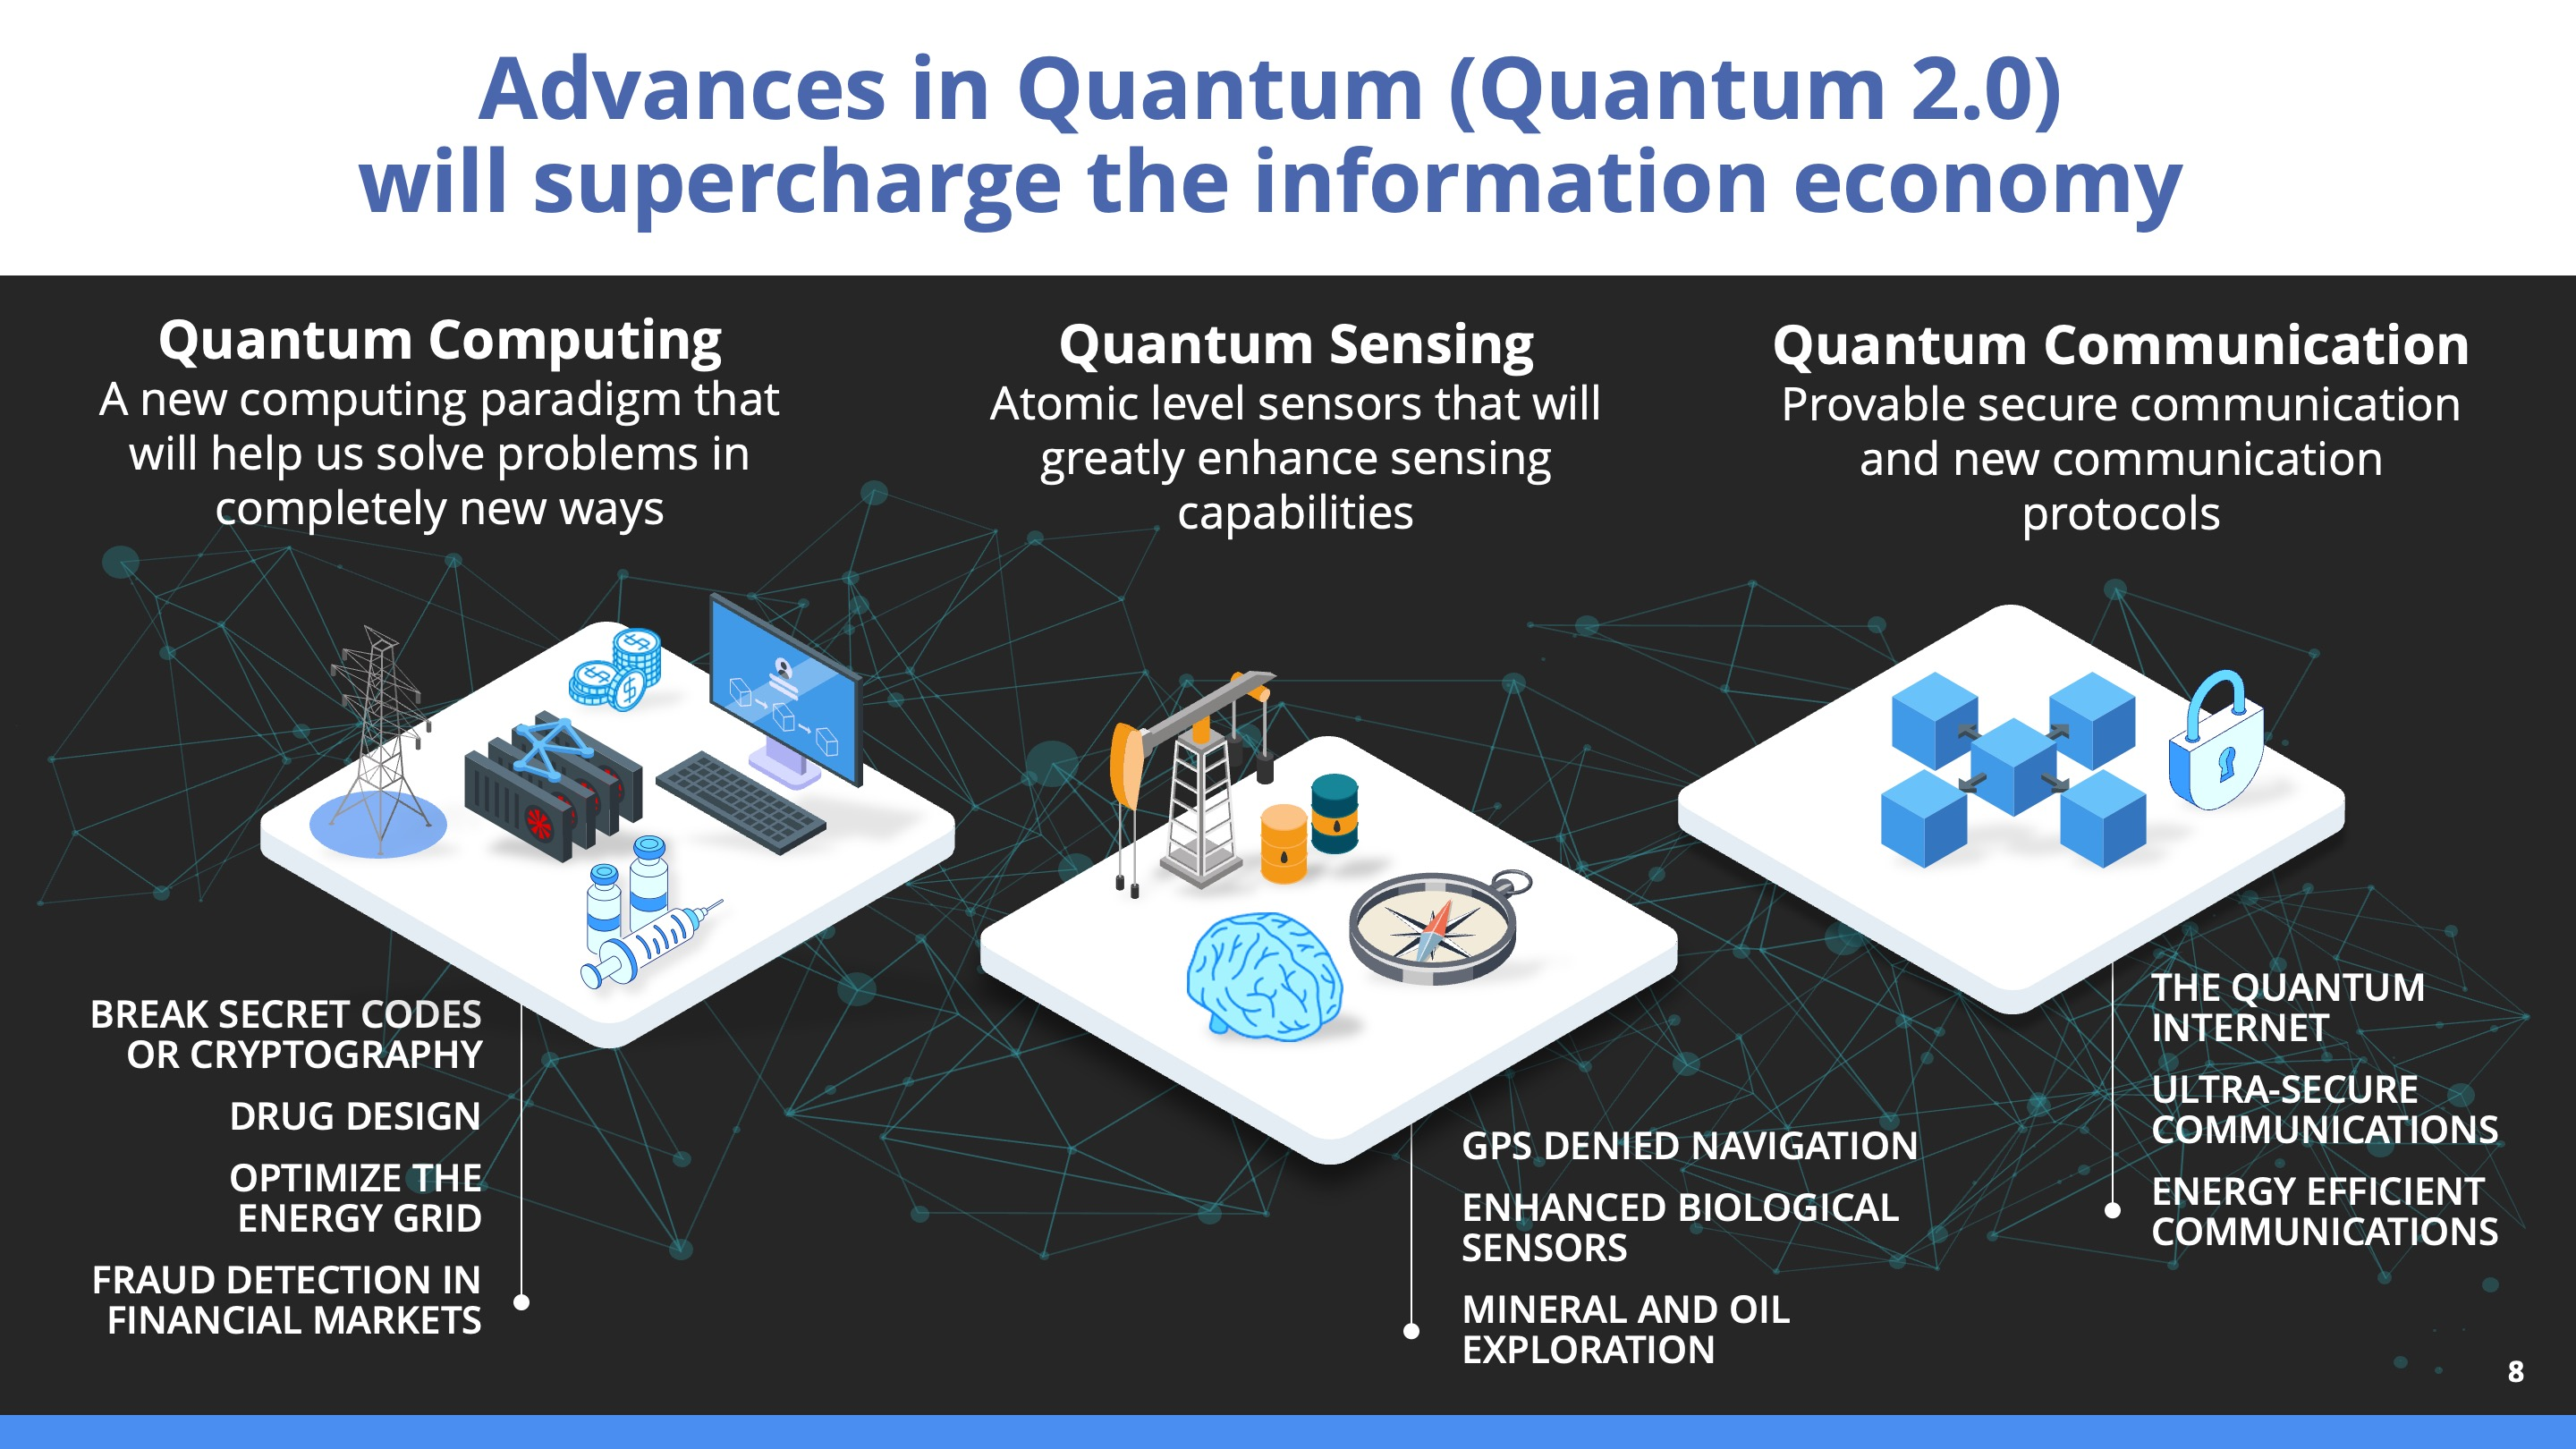
\includegraphics[width=12cm]{fig/Slide8.jpeg}
\end{center}
\end{frame}

\begin{frame}\frametitle{Introduction}
\begin{center}
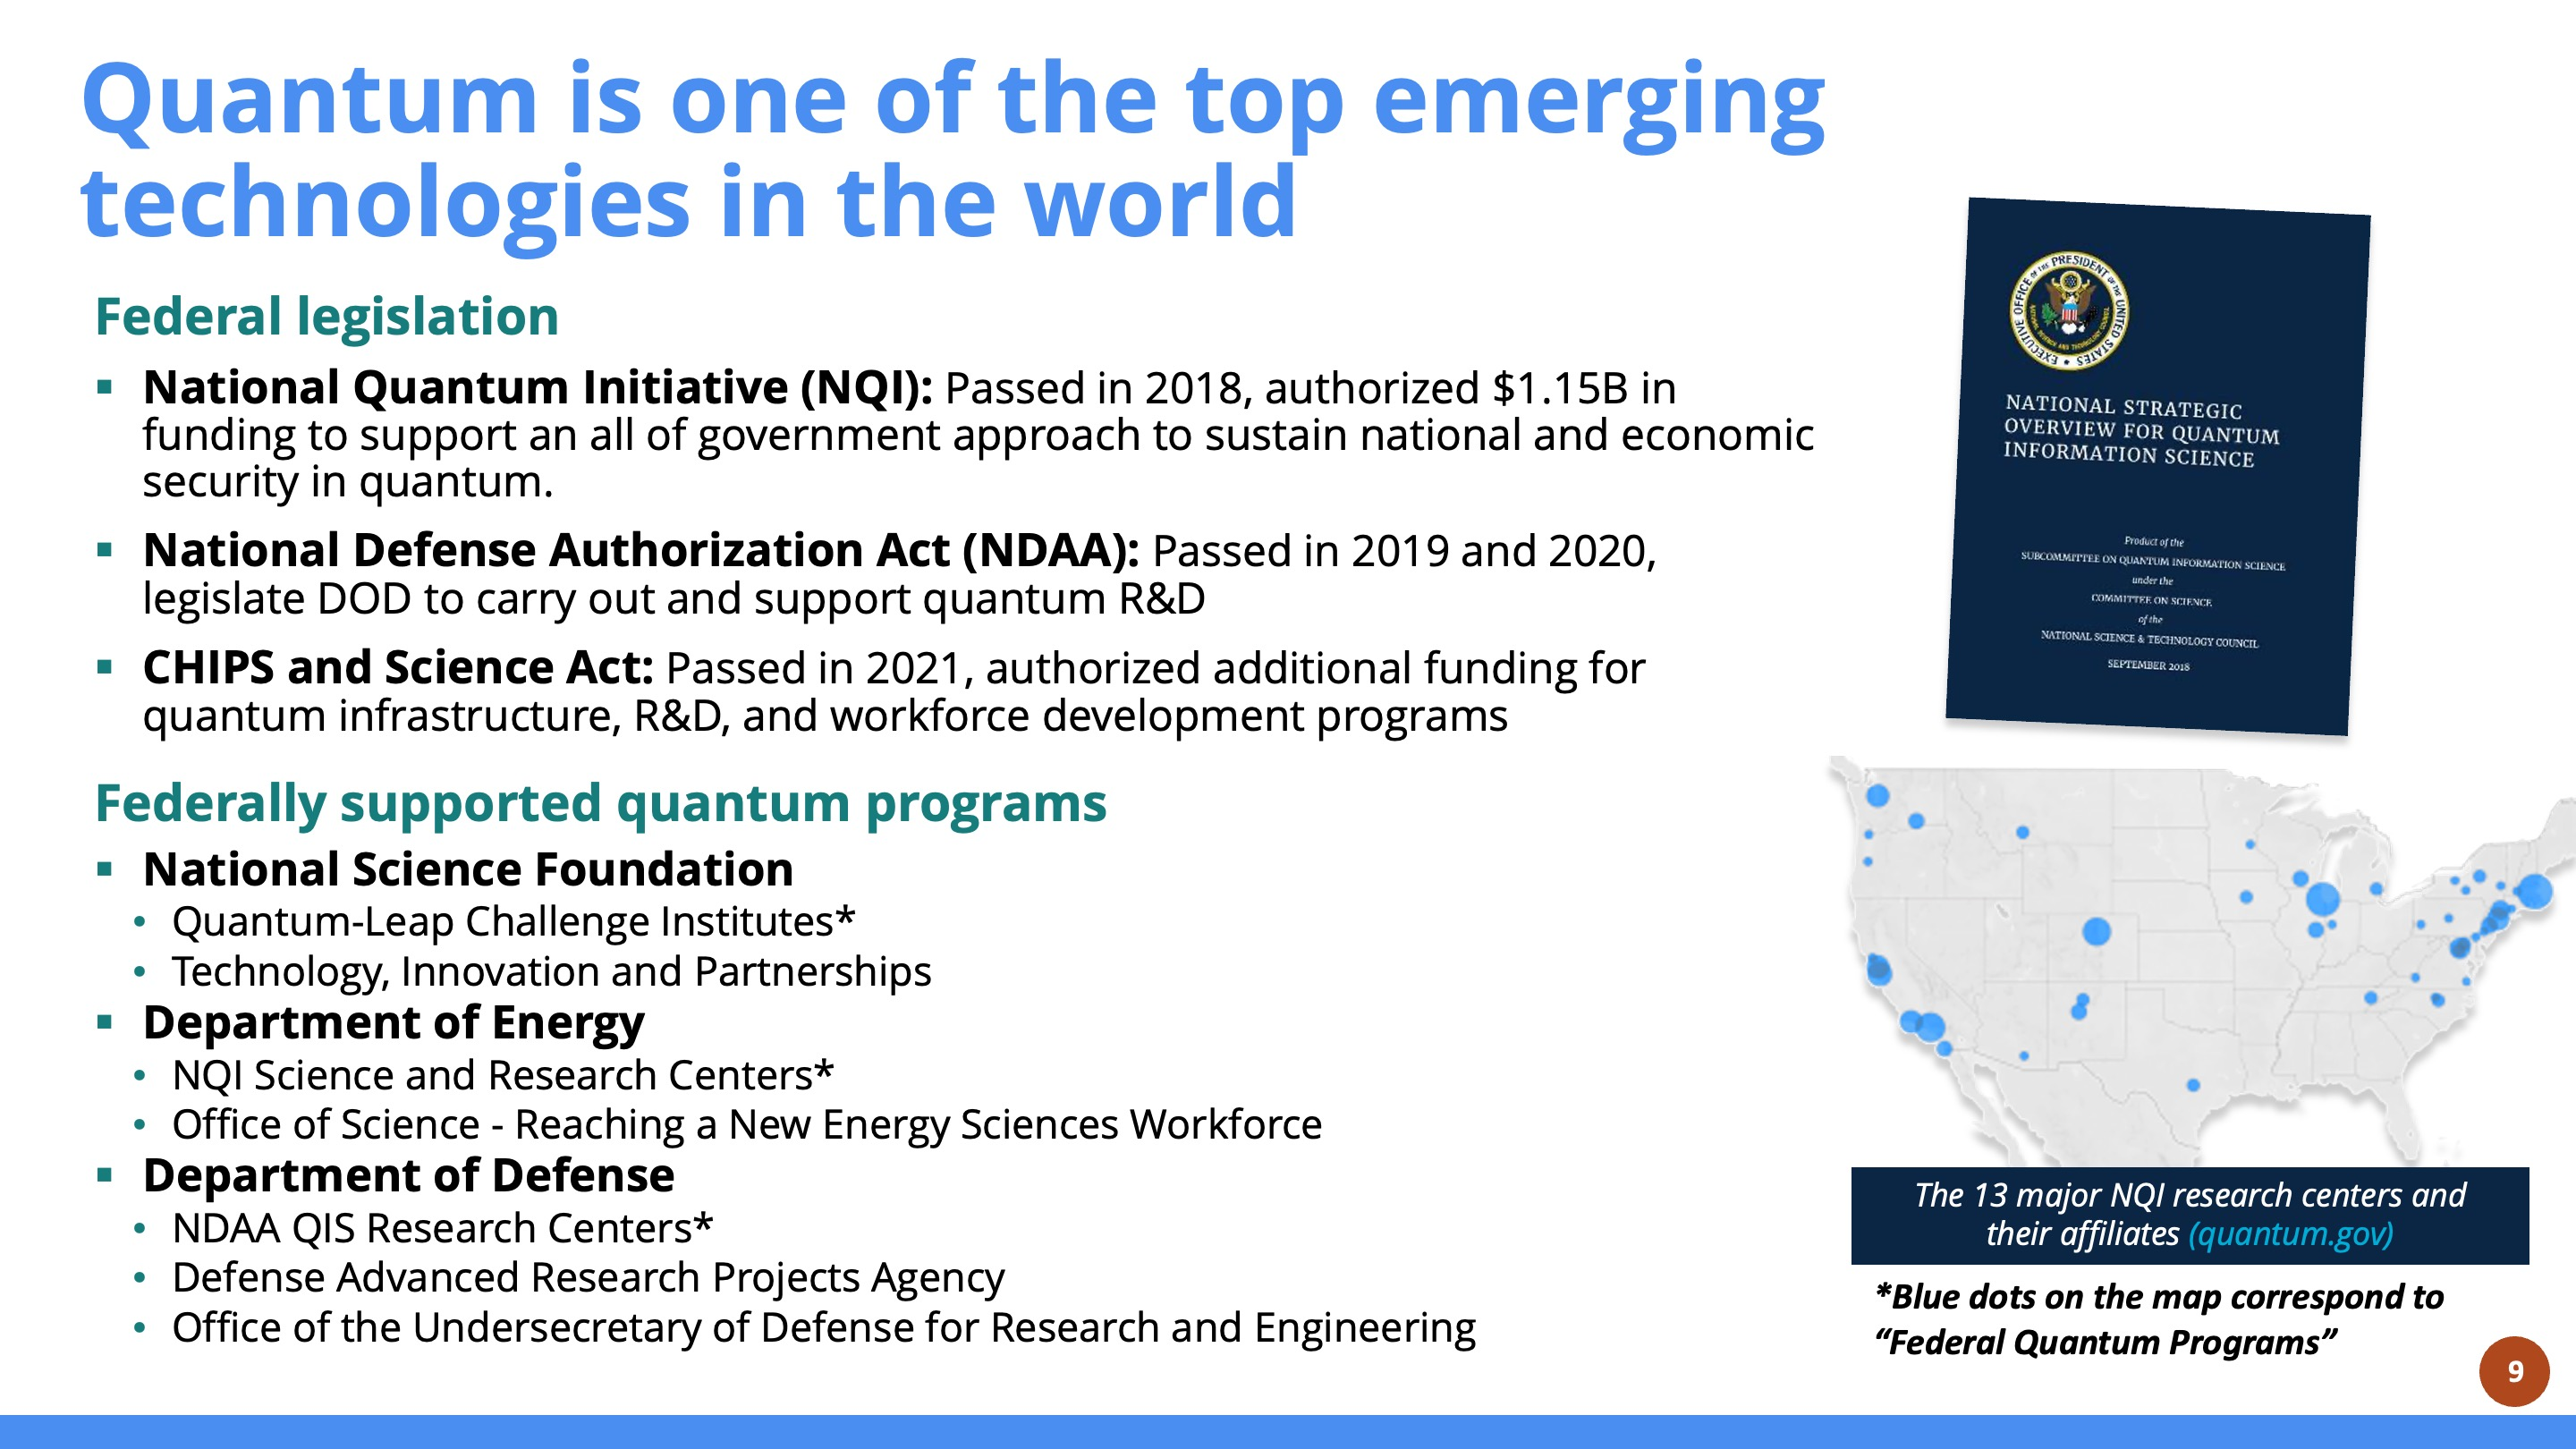
\includegraphics[width=12cm]{fig/Slide9.jpeg}
\end{center}
\end{frame}

\begin{frame}\frametitle{Introduction}
\begin{center}
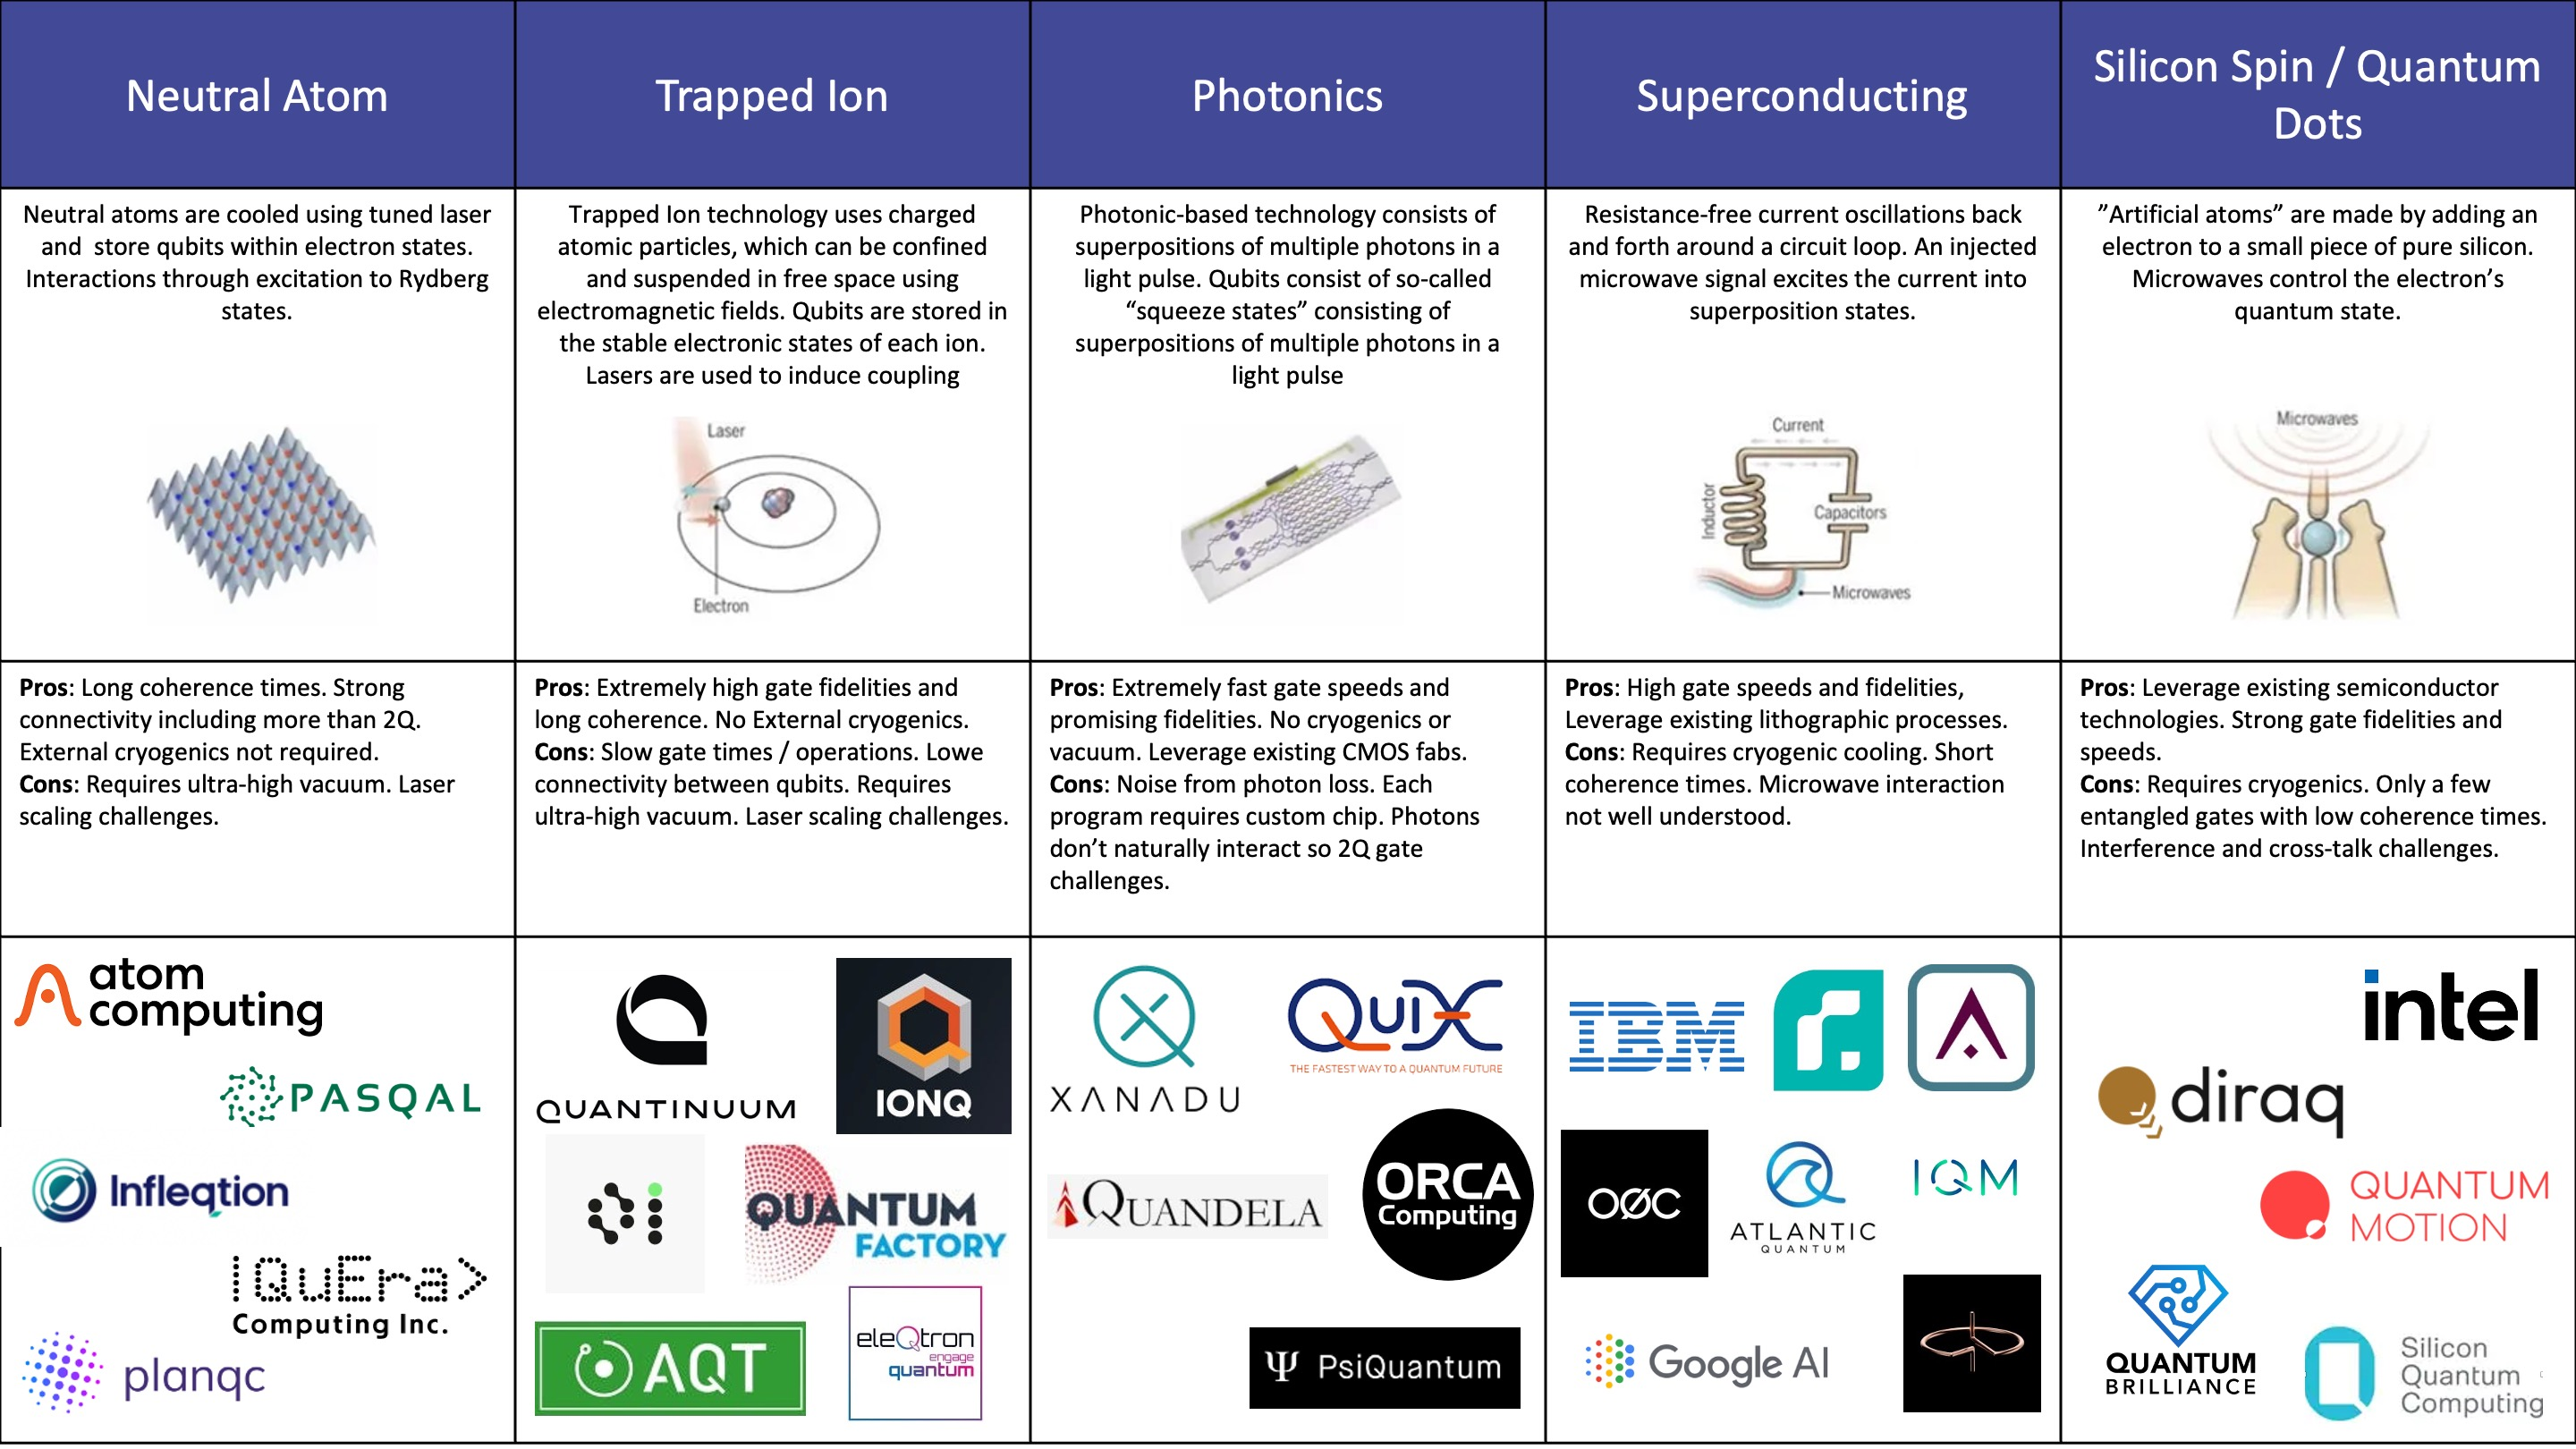
\includegraphics[width=12cm]{fig/Slide10.jpeg}
\end{center}
\end{frame}

\begin{frame}\frametitle{Introduction}
\begin{center}
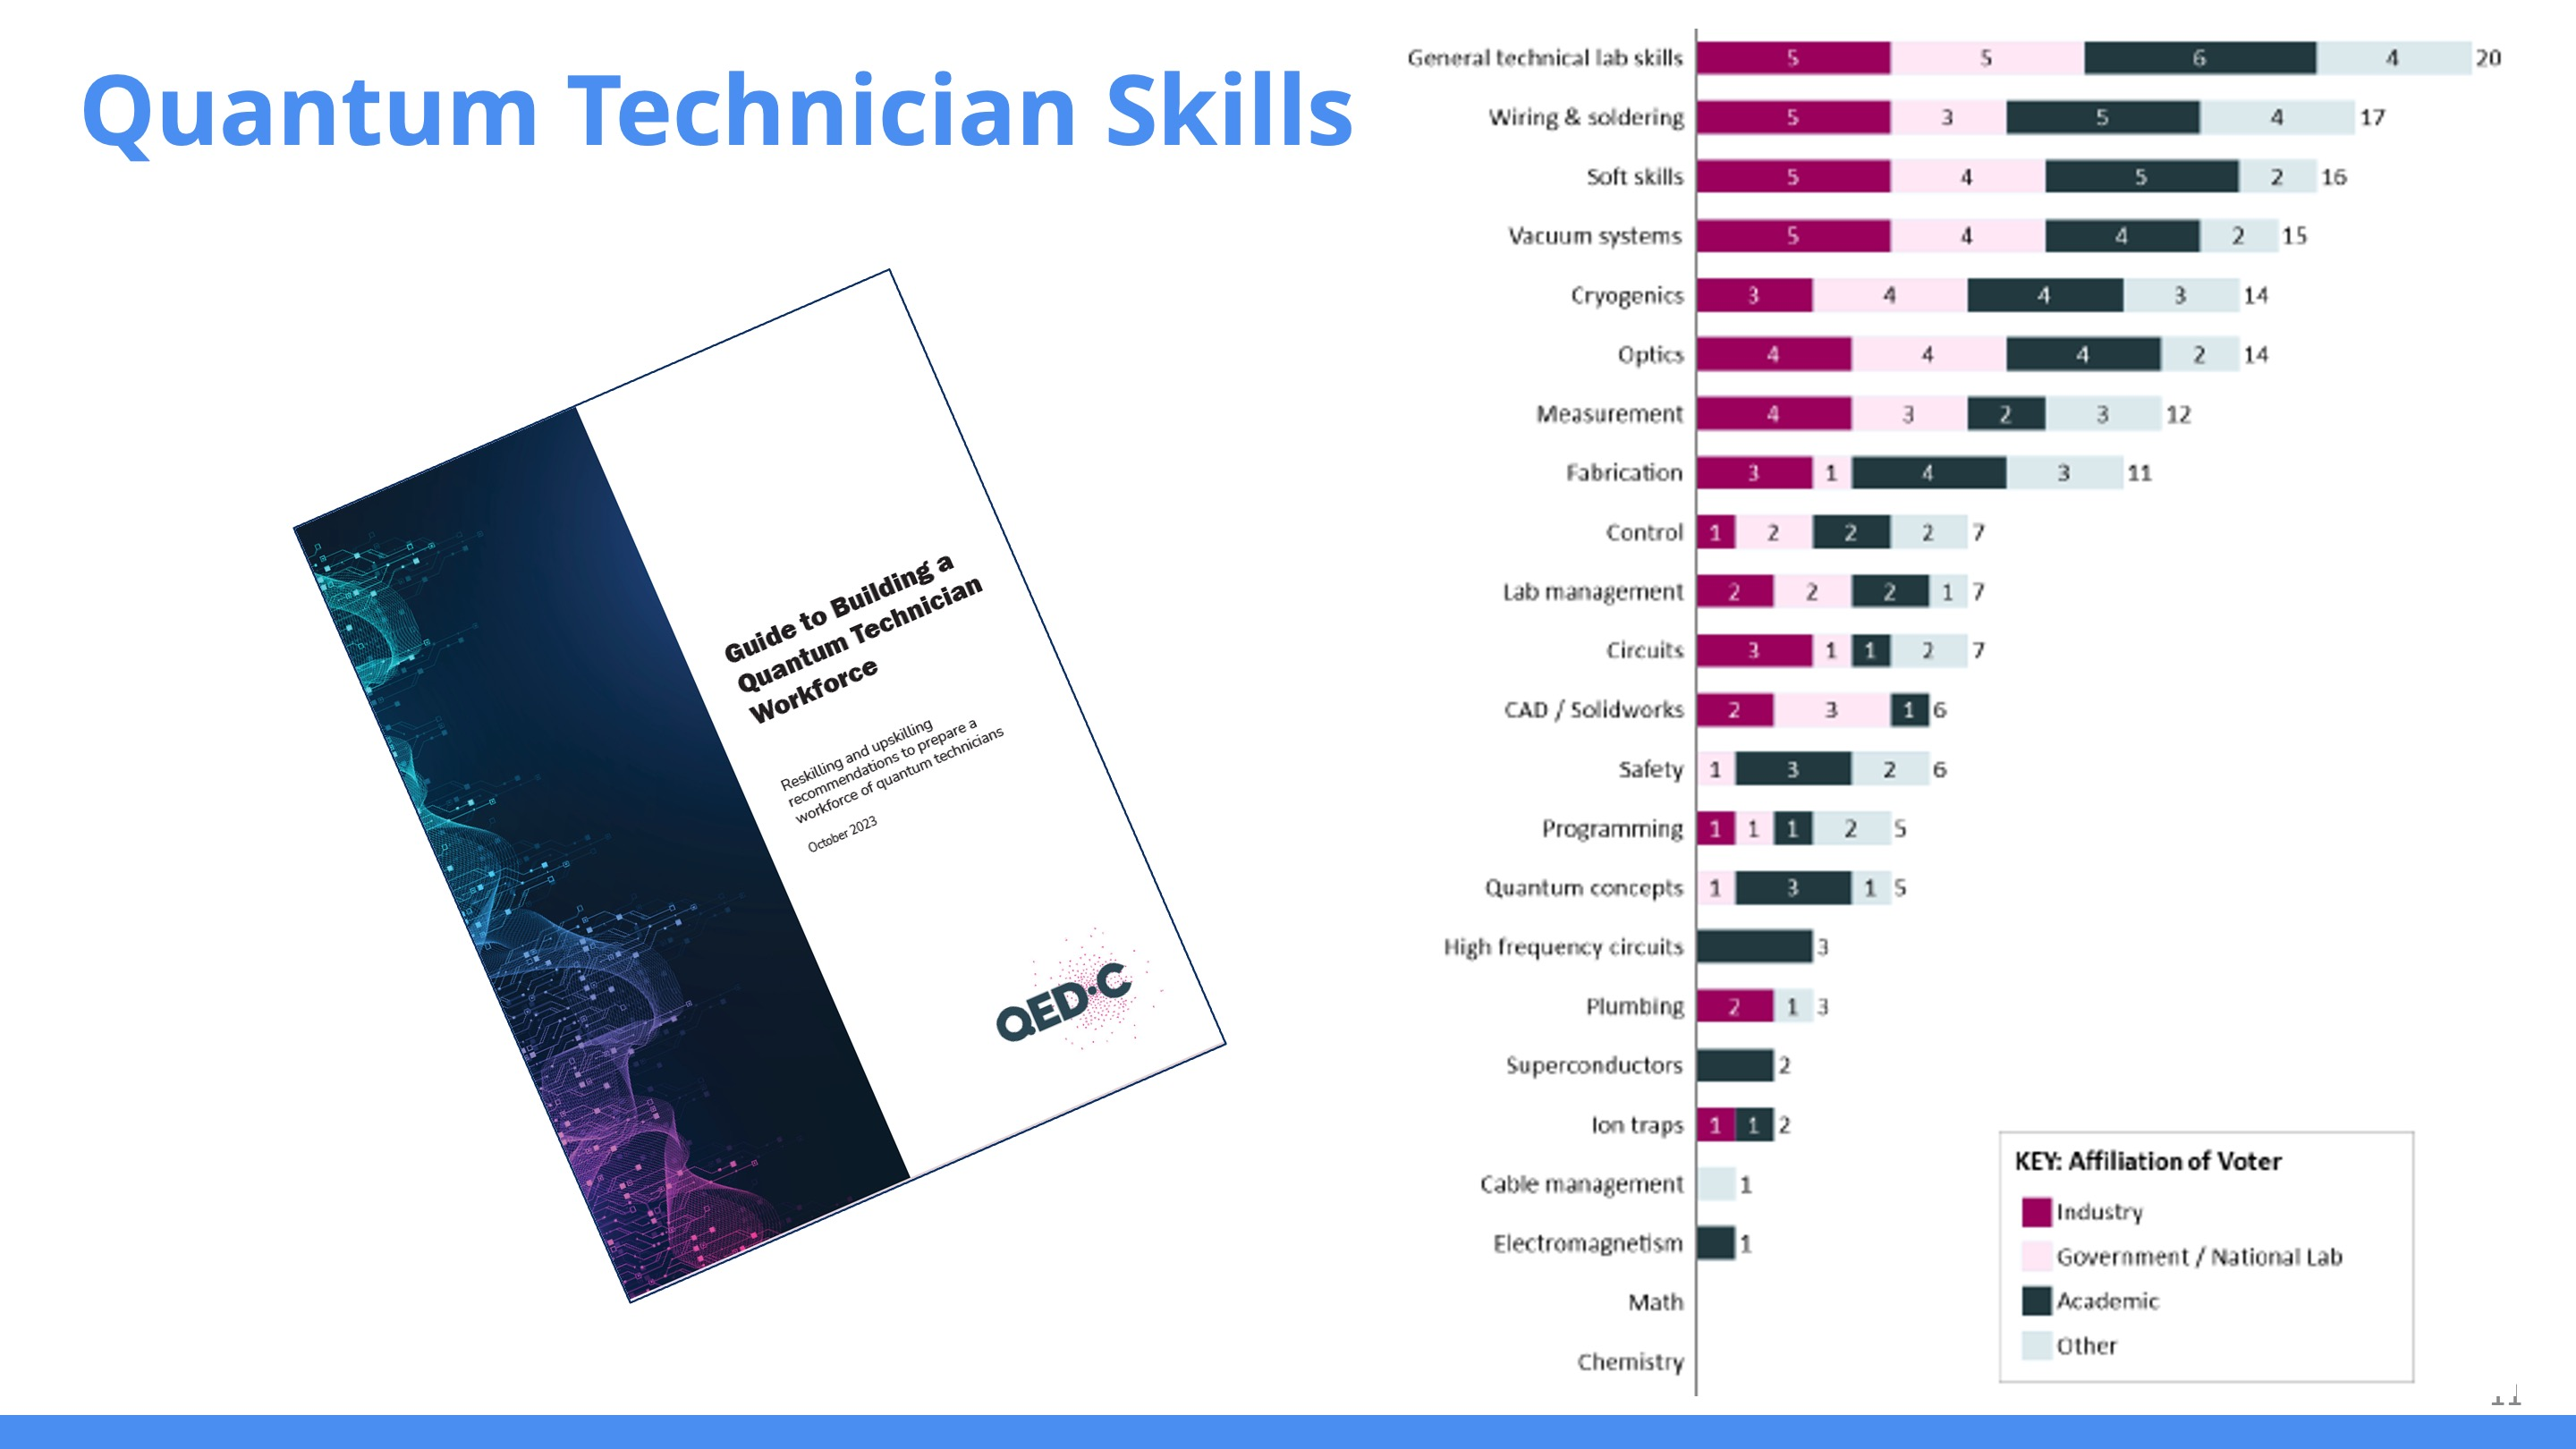
\includegraphics[width=12cm]{fig/Slide11.jpeg}
\end{center}
\end{frame}



\begin{frame}\frametitle{Introduction}
\begin{center}
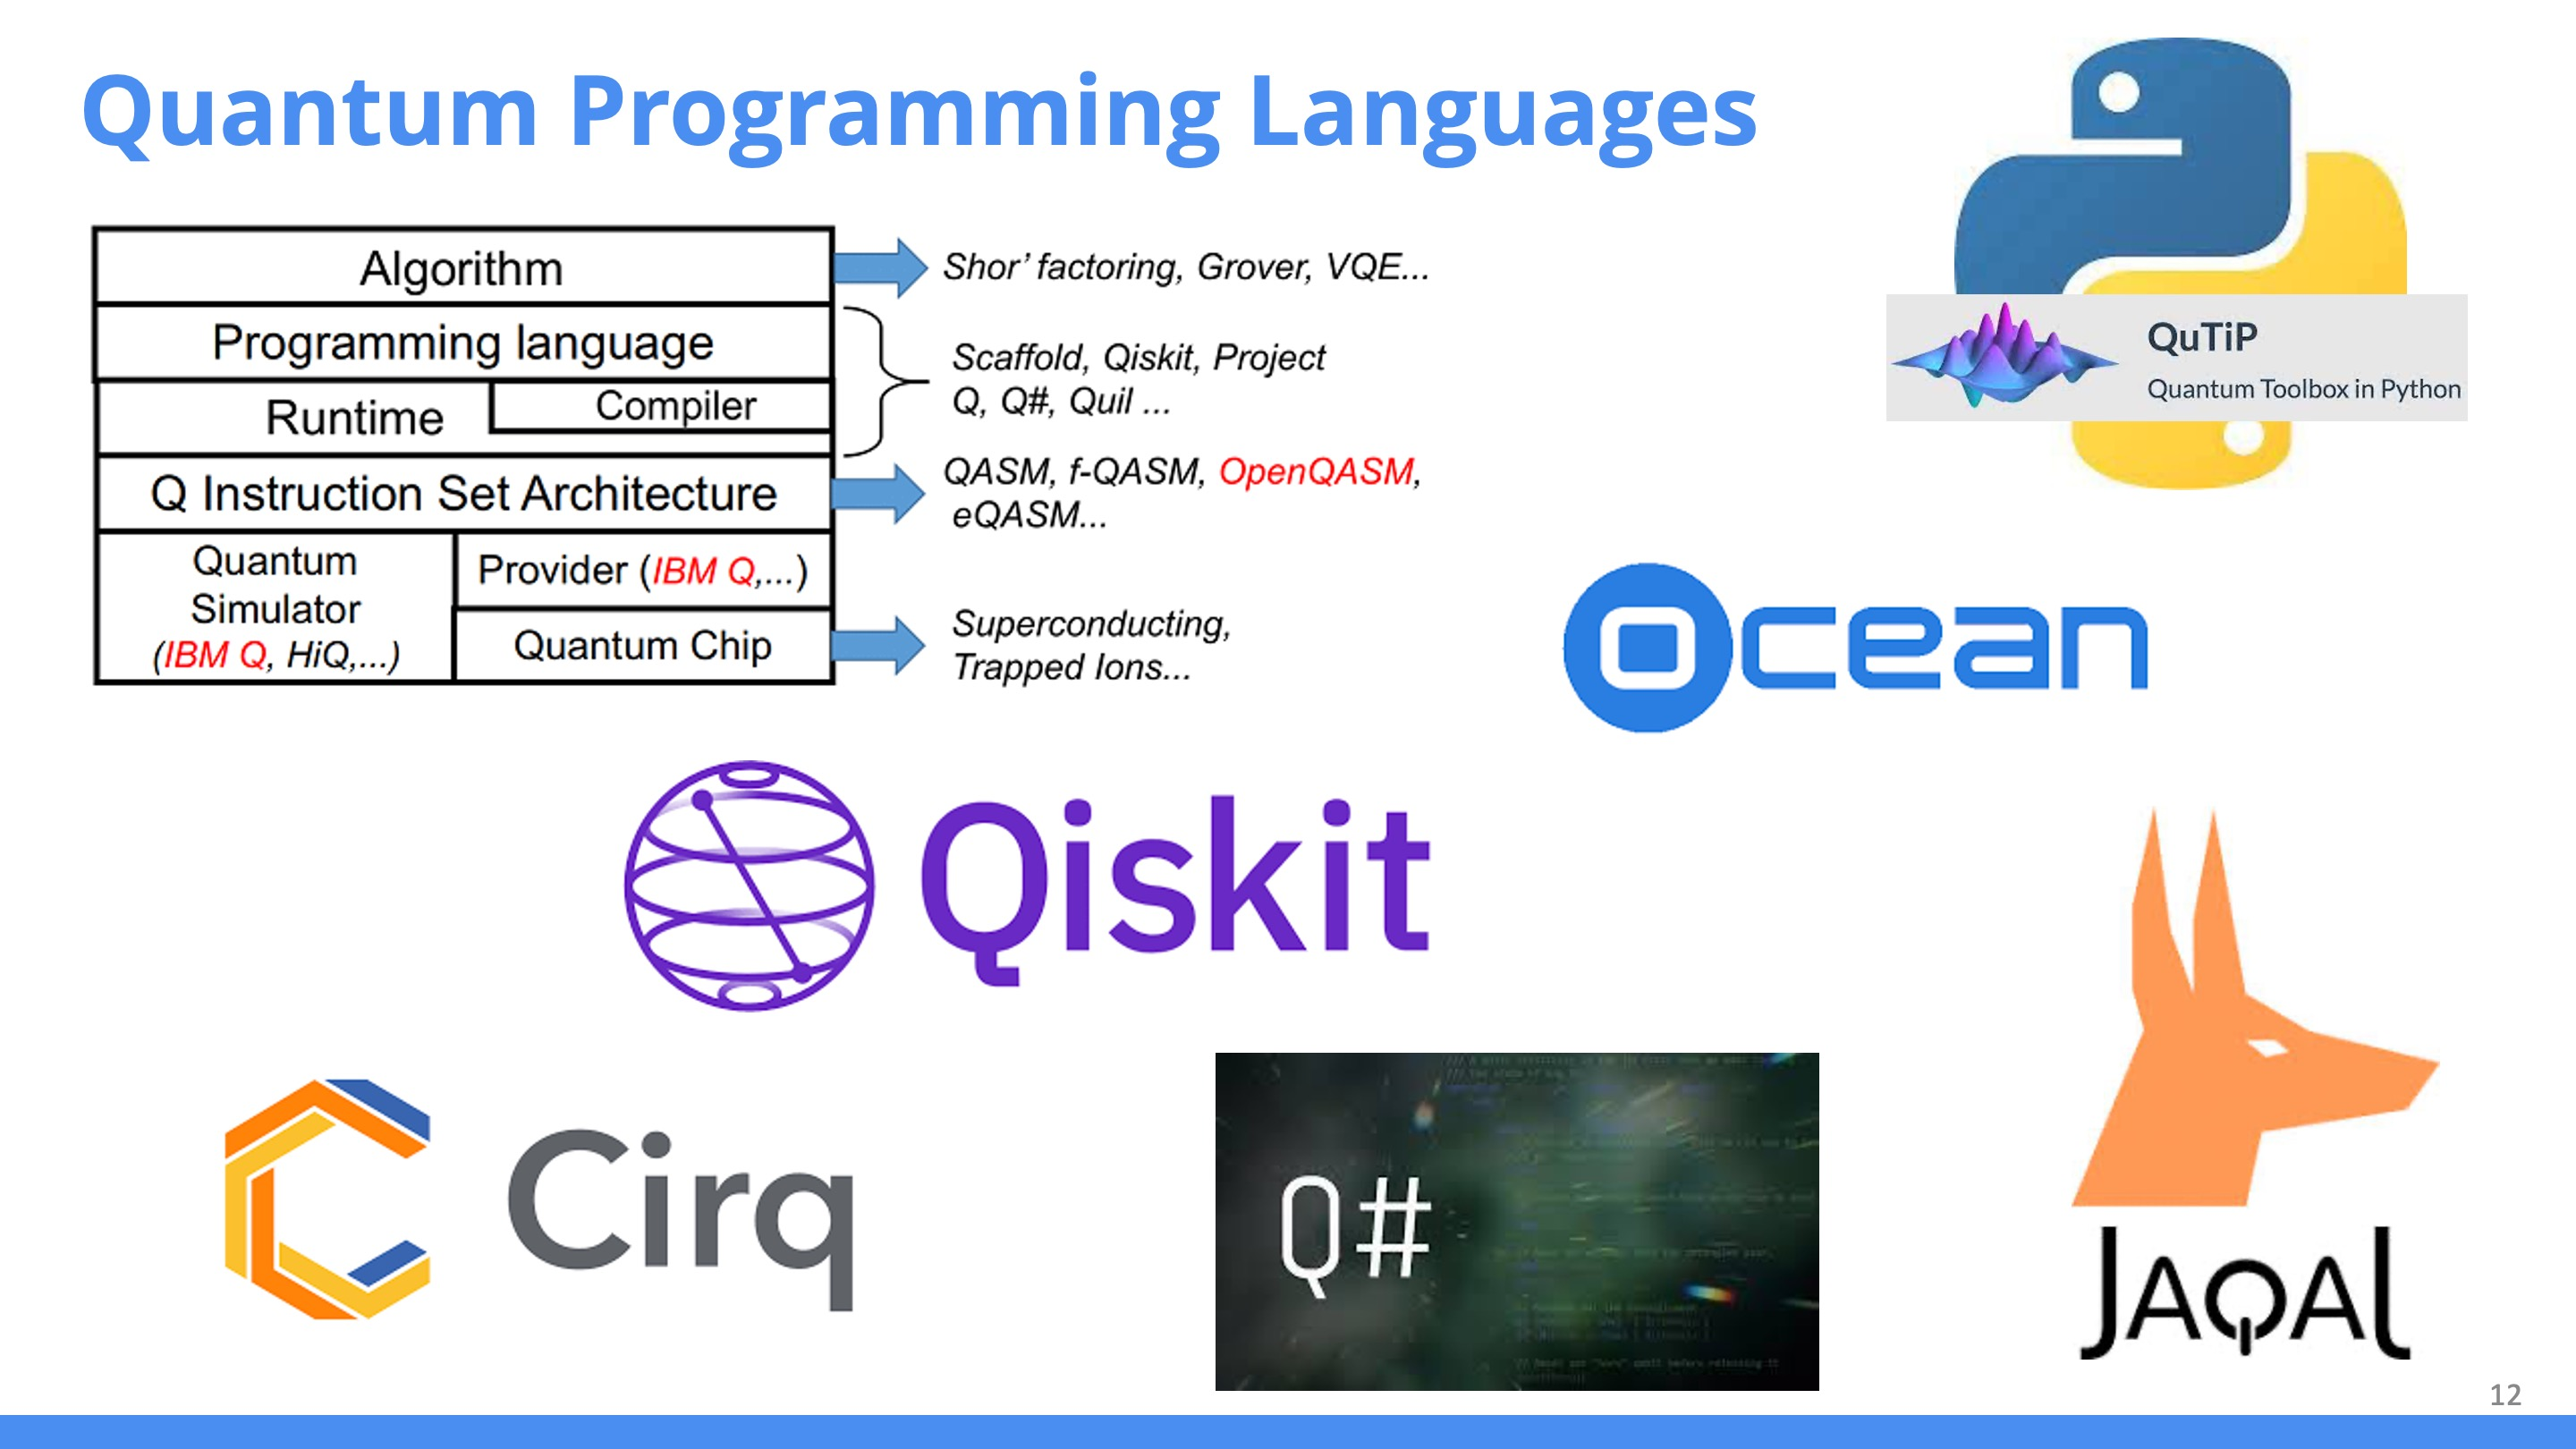
\includegraphics[width=12cm]{fig/Slide12.jpeg}
\end{center}
\end{frame}

\begin{frame}\frametitle{Introduction}
\begin{center}
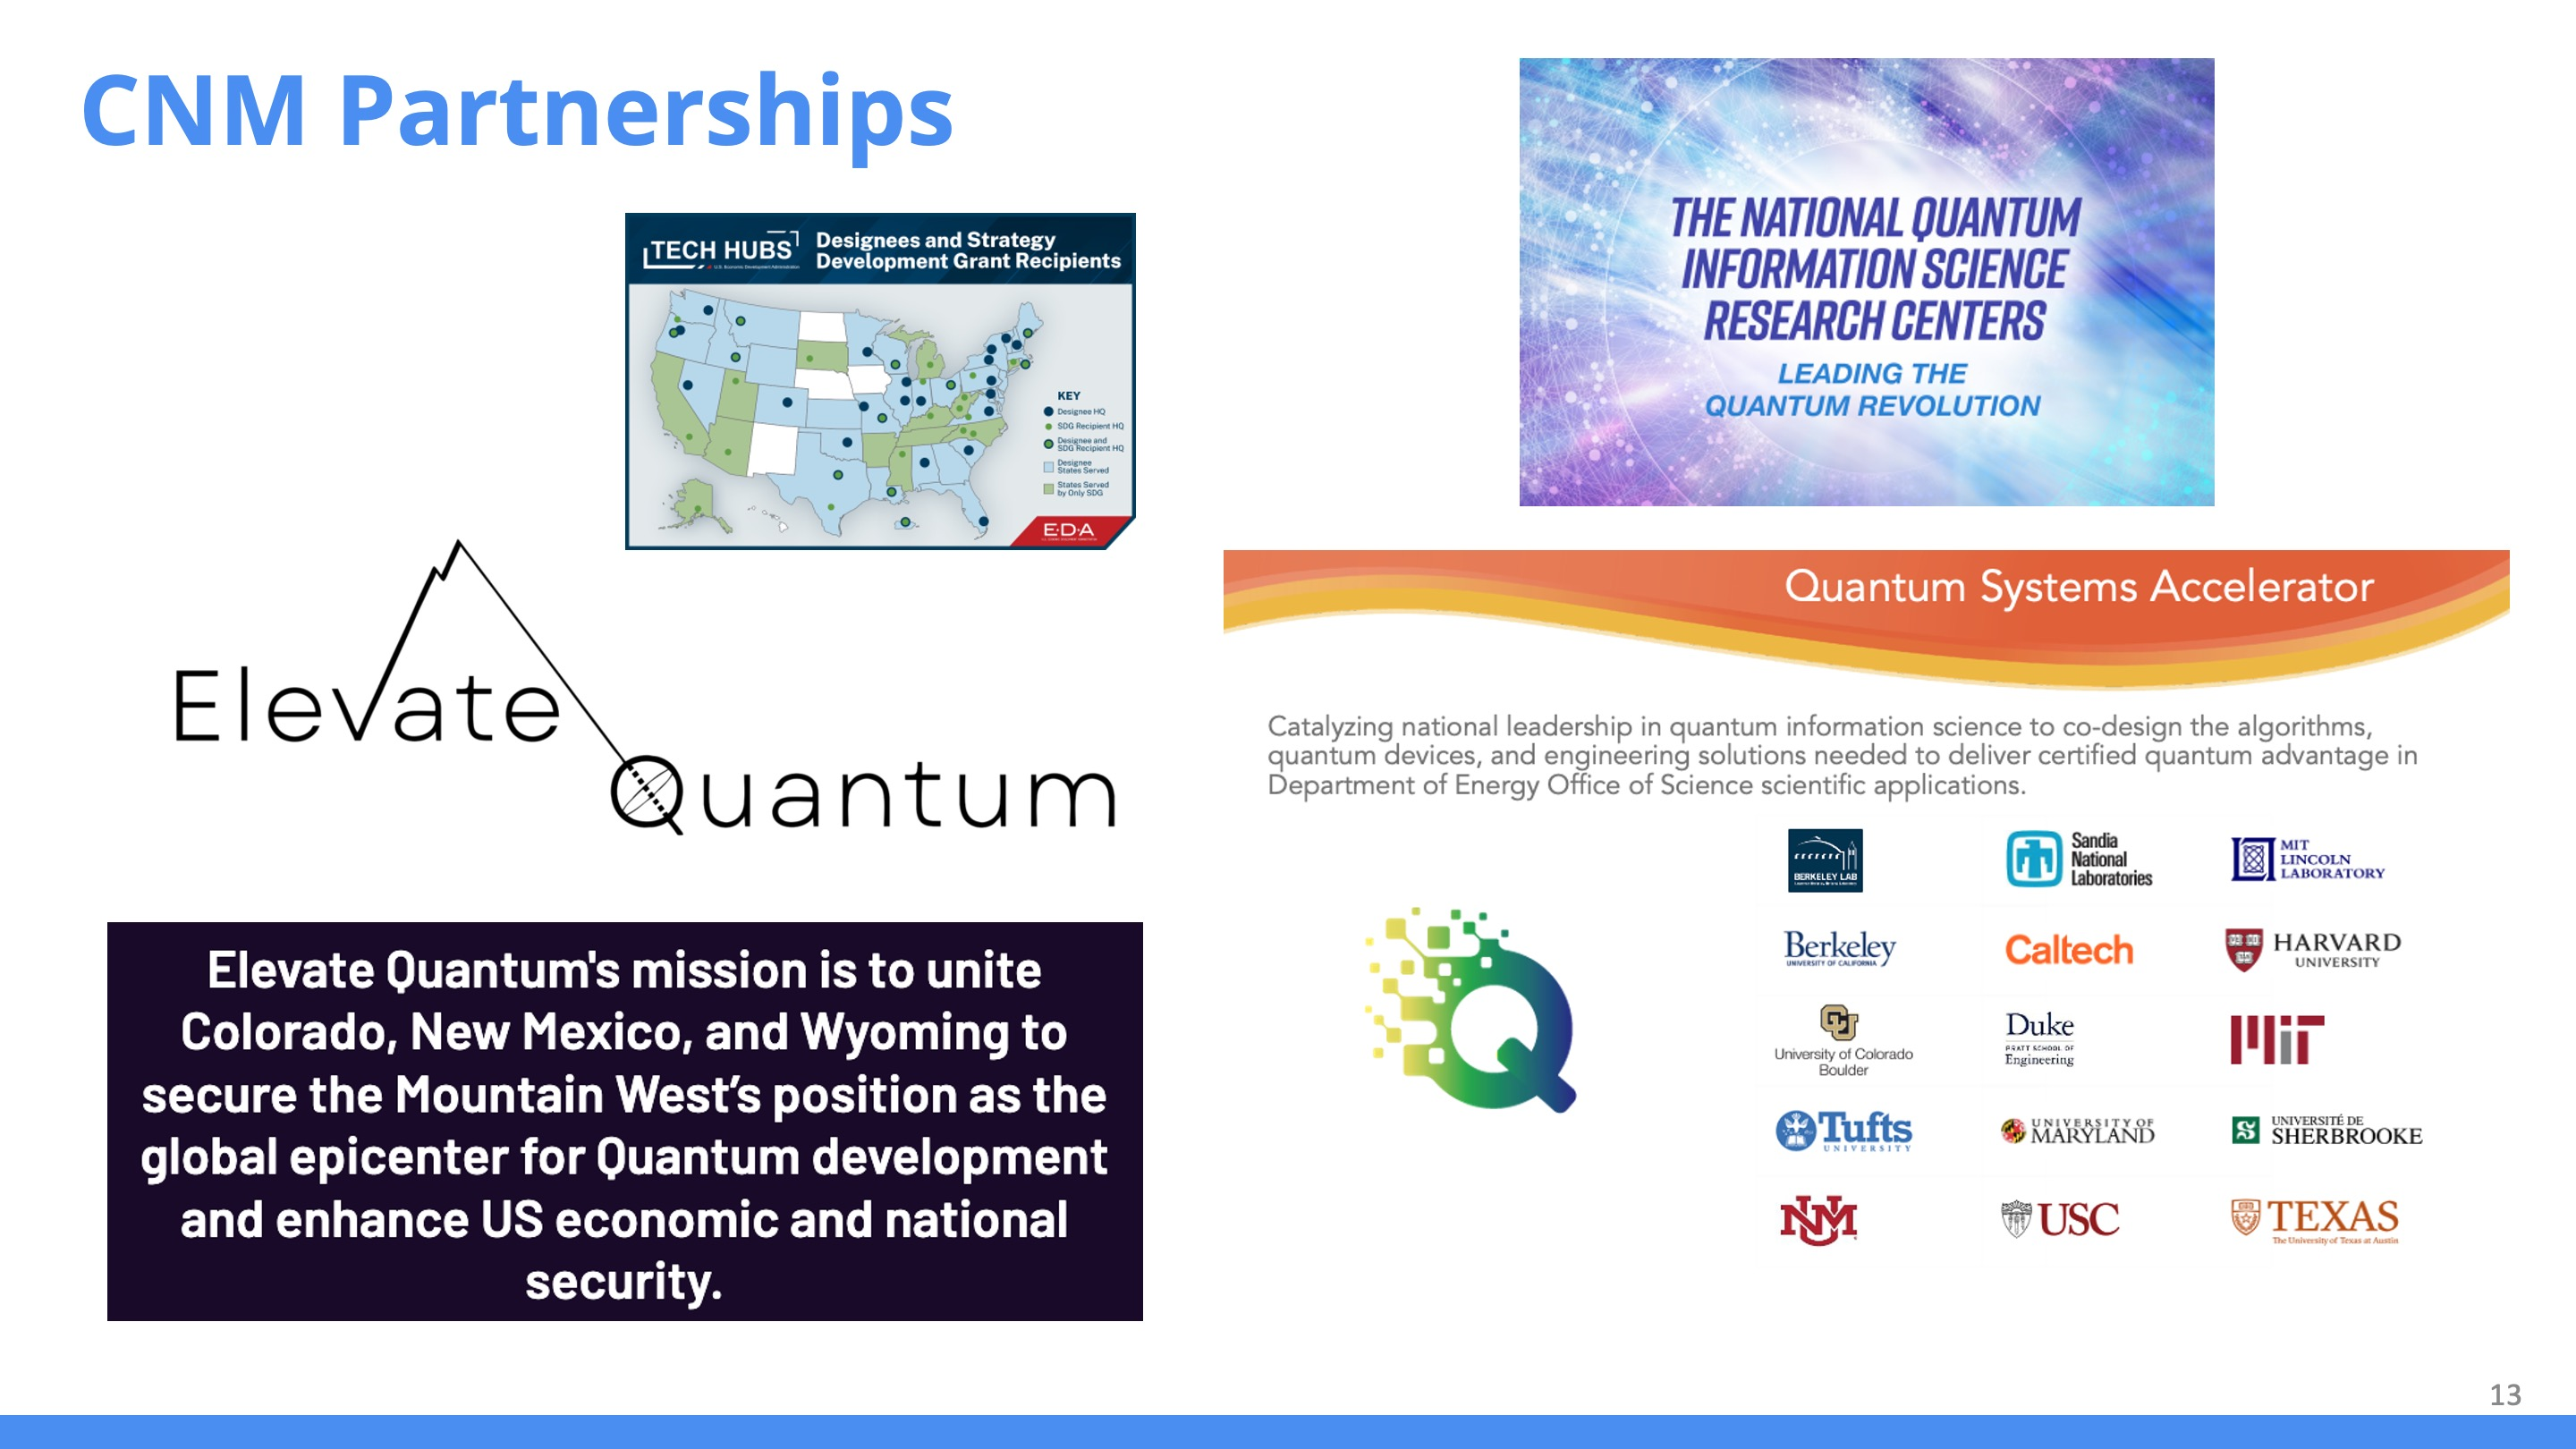
\includegraphics[width=12cm]{fig/Slide13.jpeg}
\end{center}
\end{frame}

\begin{frame}\frametitle{Introduction}
\begin{center}
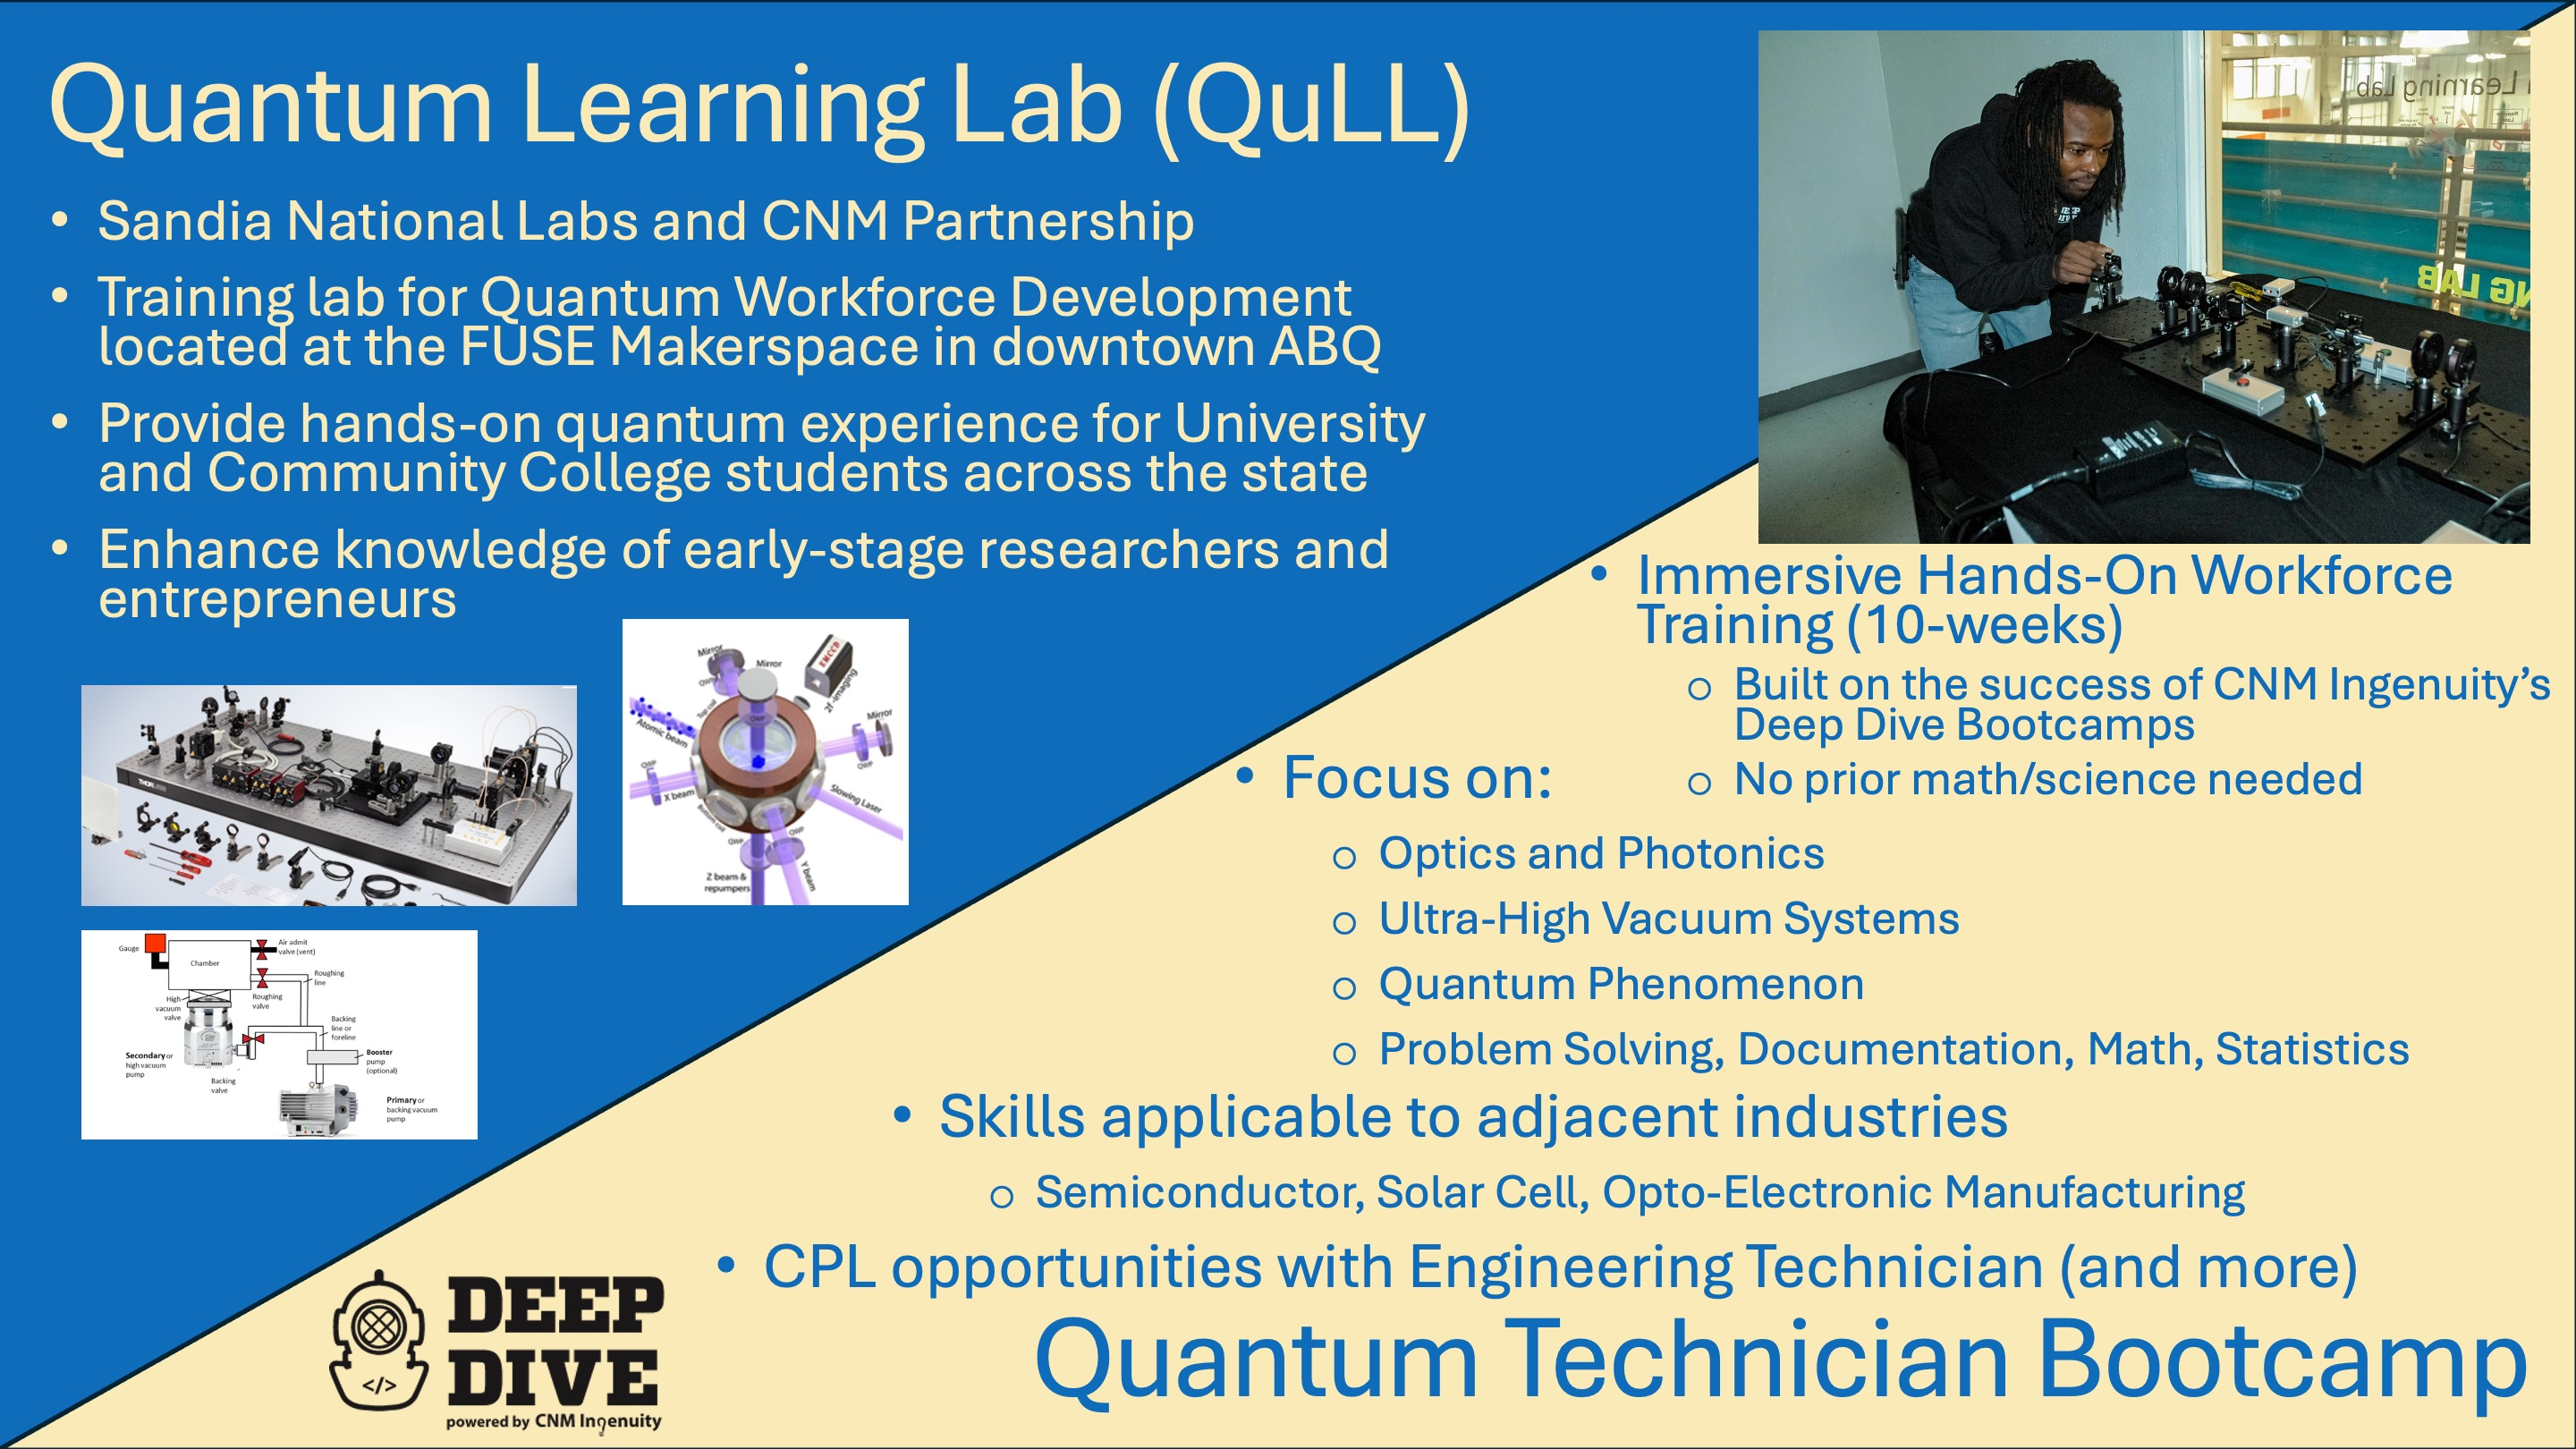
\includegraphics[width=12cm]{fig/Slide14.jpeg}
\end{center}
\end{frame}



\begin{frame}\frametitle{Introduction}
\begin{center}
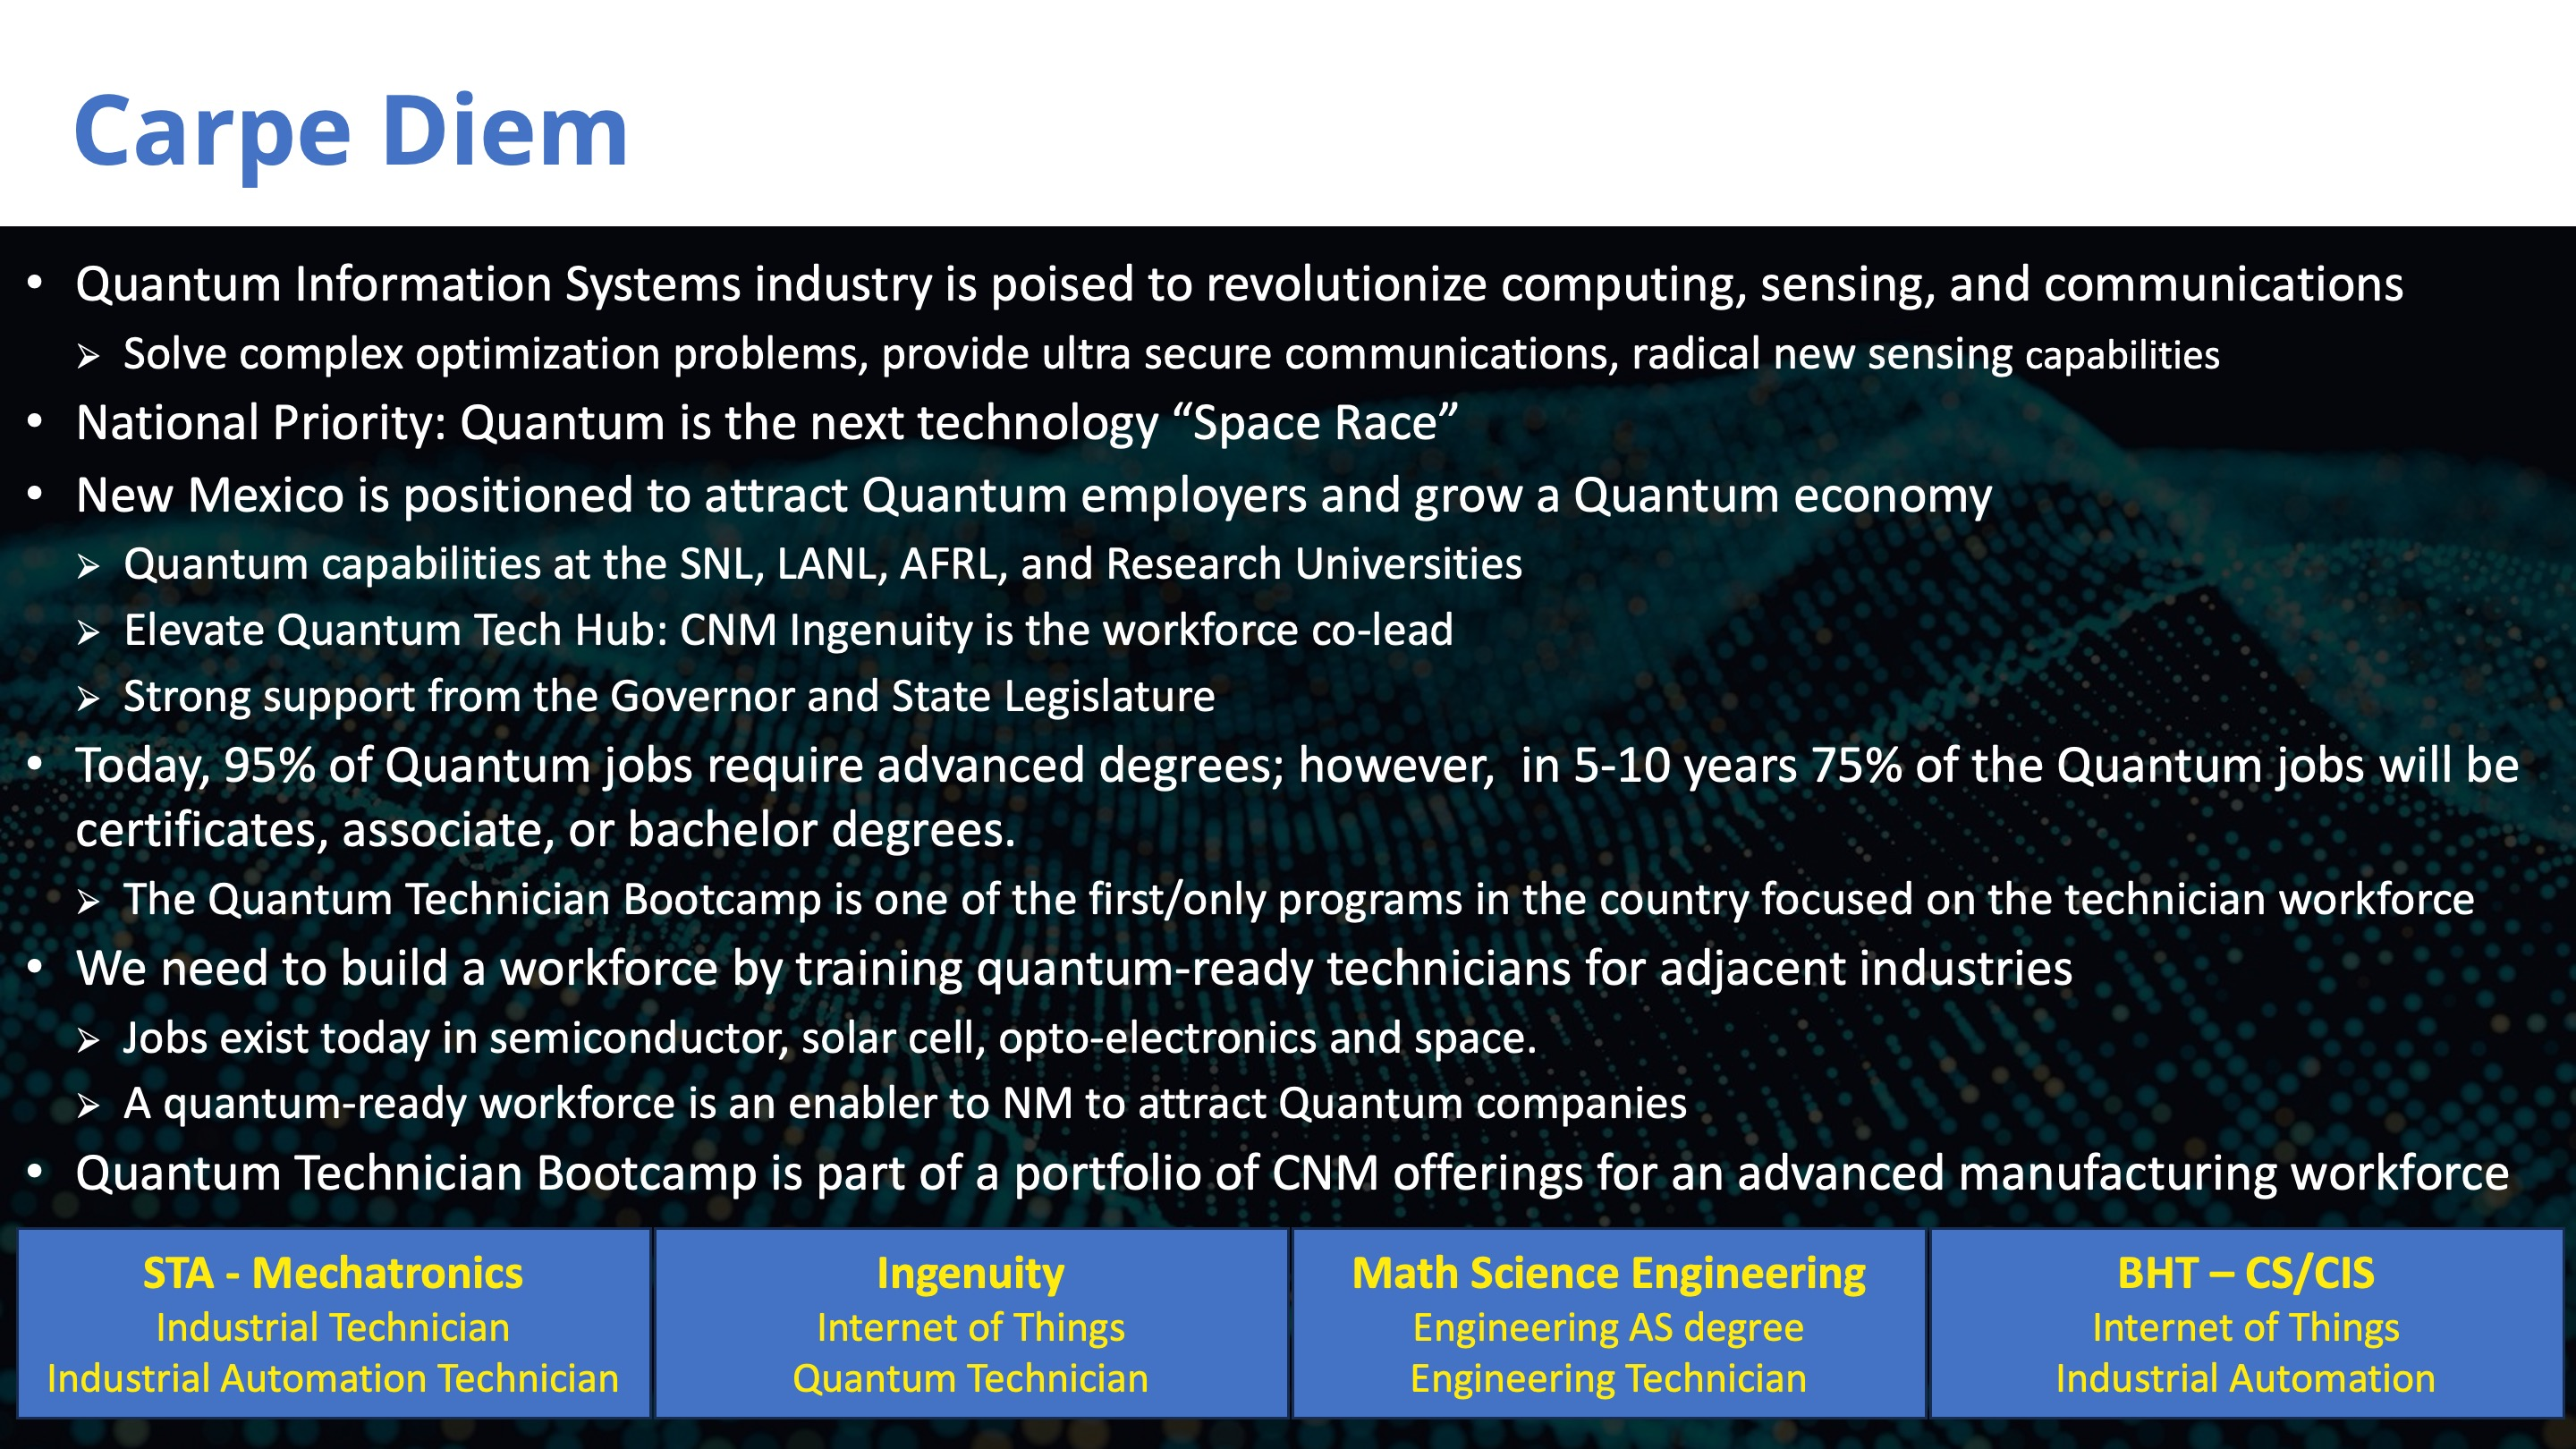
\includegraphics[width=12cm]{fig/Slide15.jpeg}
\end{center}
\end{frame}

\section{Course Overview}

\begin{frame}\frametitle{Overview}
\begin{itemize}
\item Optics
\item Lasers / Photonics
\item Ultra-High Vacuum Systems
\item Quantum Phenomenon
\item Applied Mathematics
\end{itemize}
\end{frame}

\begin{frame}\frametitle{Optics}
\begin{itemize}
\item Lab Safety and Handling of Optical Components
\item Reflection and Refraction: Prisms, Waveguides, and Dispersion
\item Focusing, Imaging, and the Paraxial Approximation
\item Thin Lens
\item Think Lens and Compound Lens
\item Apertures, Stops, Pupils, Windows
\item Mirrors: Convex, Concave
\item Cameras: Focusing, Resolution, and Contrast
\item Aberrations
\item Telescopes / Microscopy
\item Spectra and Filters
\end{itemize}
\end{frame}

\begin{frame}\frametitle{Laser and Photonics}
\begin{itemize}
\item Laser  Safety
\item Introduction to Lasers and Atomic Energy Levels
\item Beam Properties: laser modes, beam profile, and coherence.
\item Interferometry
\item Polarization – polarizers, half/quarter wave plates
\item Optical intensity. Single-mode and multi-mode optical fibers
\item Optical detectors: photodiode, photomultiplier tubes, avalanche photodiodes, infrared detectors
\item Optical spectra and emission spectroscopy
\item Absorption Spectroscopy
\item Optical Tweezers
\item Industrial Applications of Laser and Photonics
\end{itemize}
\end{frame}

\begin{frame}\frametitle{Ultra-High Vacuum Systems}
\begin{itemize}
\item Vacuum System Safety including Lock-out Tag-out (LOTO) of electrical and mechanical hazards
\item Foundations of Vacuum Technology
\item Vacuum Pump Technologies – Displacement: Backing Pumps, Turbomolecular Pumps.
\item Vacuum Measurement: Pirani and Ion Gauges
\item Vacuum System Assembly
\item Vacuum System Contamination
\item Leak Detection
\item High Vacuum vs Ultra-High Vacuum

\end{itemize}
\end{frame}

\begin{frame}\frametitle{Quantum Phenomenon}
\begin{itemize}
\item Introduction to Quantum 
\item Superposition, Quantum Gates
\item Entanglement
\item Particle/Wave Dual Nature of Light, Polarization, and Quantum Eraser
\item Quantum Measurements
\item Cryogenics
\item Superconducting and Spin Qubits
\item Laser Cooling
\item Atomic, Molecular, and Optical Qubits
\item Neutral Atom QIS Operations
\item Quantum Sensors: Diamond NV
\end{itemize}
\end{frame}

\begin{frame}\frametitle{Applied Math}
\begin{itemize}
\item College Algebra
\item Vectors
\item Trigonometry
\item Linear Algebra
\item Statistics
\end{itemize}
\end{frame}


\section{Geometric Optics}

\begin{frame}\frametitle{Ray Nature of Light}
The word "ray" means a straight line that originates at some point.

\begin{center}
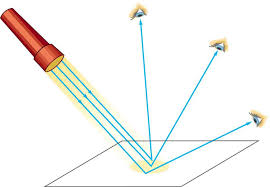
\includegraphics[width=6cm]{fig/rays.jpg}
\end{center}

The part of optics dealing with the ray aspect of light is called "geometric optics."

\end{frame}


\begin{frame}\frametitle{Reflection}
The angle of reflection equals the angle of incidences

\begin{center}
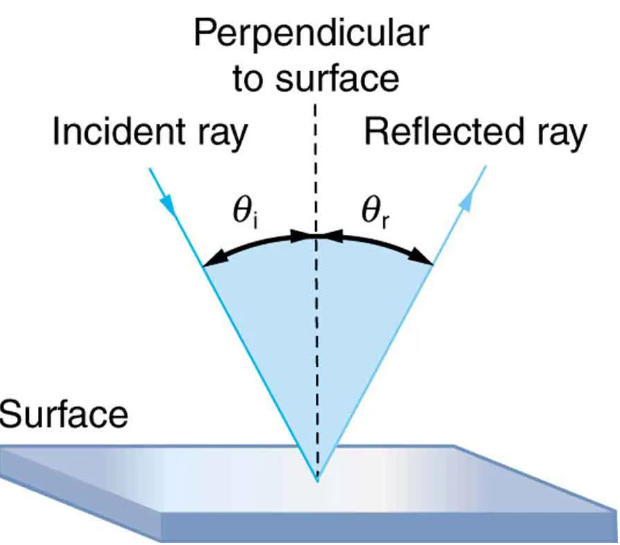
\includegraphics[width=6cm]{fig/reflect.png}
\end{center}

\end{frame}


\begin{frame}\frametitle{Rough vs Smooth Surfaces}

\begin{center}
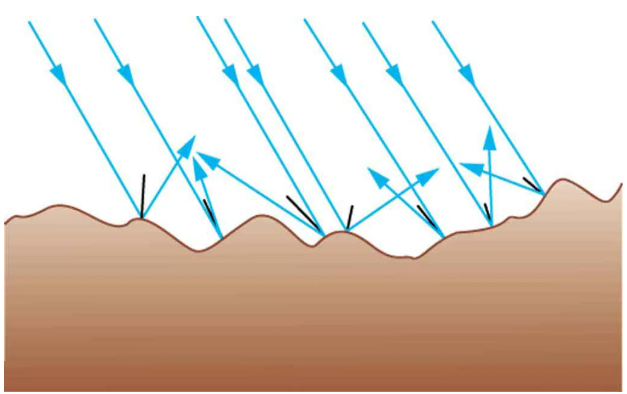
\includegraphics[width=3.5cm]{fig/reflect_rough.png}
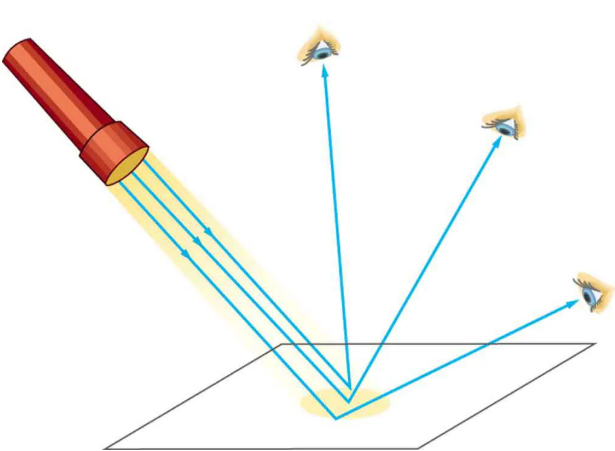
\includegraphics[width=3.5cm]{fig/reflect_paper.png}
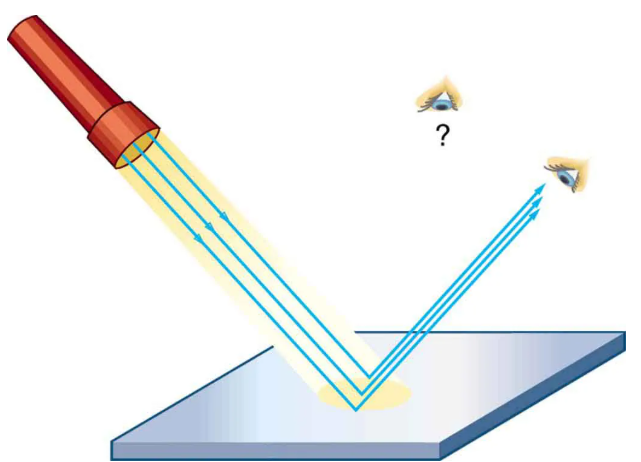
\includegraphics[width=3.5cm]{fig/reflect_mirror.png}
\end{center}

\end{frame}

\begin{frame}\frametitle{Mirrors and Virtual Images}
When we see ourselves in a mirror, it appears that our image is actually behind the mirror.

\begin{center}
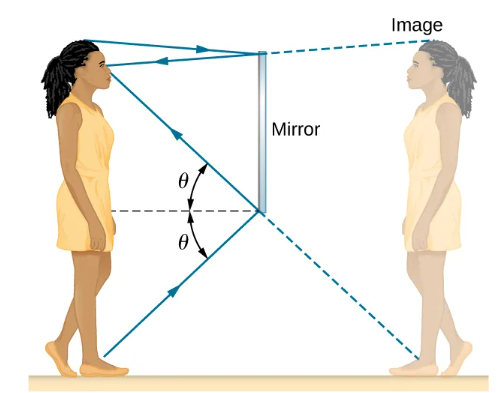
\includegraphics[width=6cm]{fig/virtual.png}
\end{center}

\end{frame}

\begin{frame}\frametitle{Speed of Light}
\begin{columns}
\begin{column}{7cm}
\begin{itemize}
\item In 1676, Danish astronomer Ole Roemer noted the change in orbital period of Jupiter's moons depending of if the earth was moving towards or away from Jupiter. He as able to calculate speed of light to be $2.26 x 10^8 (\frac{m}{s})$.
\item In 1887, American physicist Albert Michelson used a rotating mirror to get a more precise measurement of the speed of light. 
\item Today, the speed of light is known as:
\end{itemize}
\begin{center}
$c=2.99792458×10^8 (\frac{m}{s})$.
\end{center}

\end{column}
\begin{column}{5cm}
\begin{center}
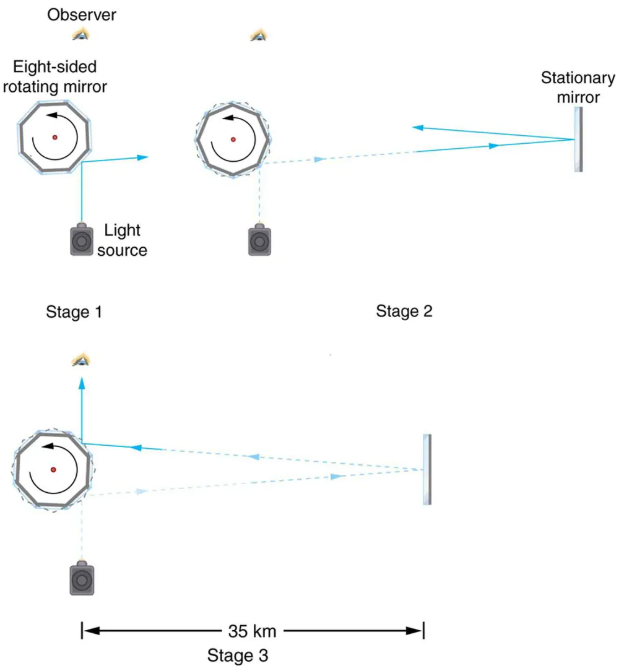
\includegraphics[width=4.5cm]{fig/c_meas.png}
\end{center}
\end{column}
\end{columns}
\end{frame}


\begin{frame}\frametitle{Two Mirror Walk}
\begin{columns}
\begin{column}{8cm}
\begin{itemize}
\item Center of first mirror should match incoming height of incoming beam path and the second mirror set to the height of of the target beam path.
\item Set alignment target at height of target.
\item Course adjust both mirrors by hand.
\item Place the alignment target along the beampath to the target
\item Fine tune the beampath by using the adjusters on both mirrors. Note: adjusting the first mirror affects the placement of the second mirror. 
\item Move the alignment target along the output beampath to endure it is level
\end{itemize}

\end{column}
\begin{column}{4cm}
\begin{center}
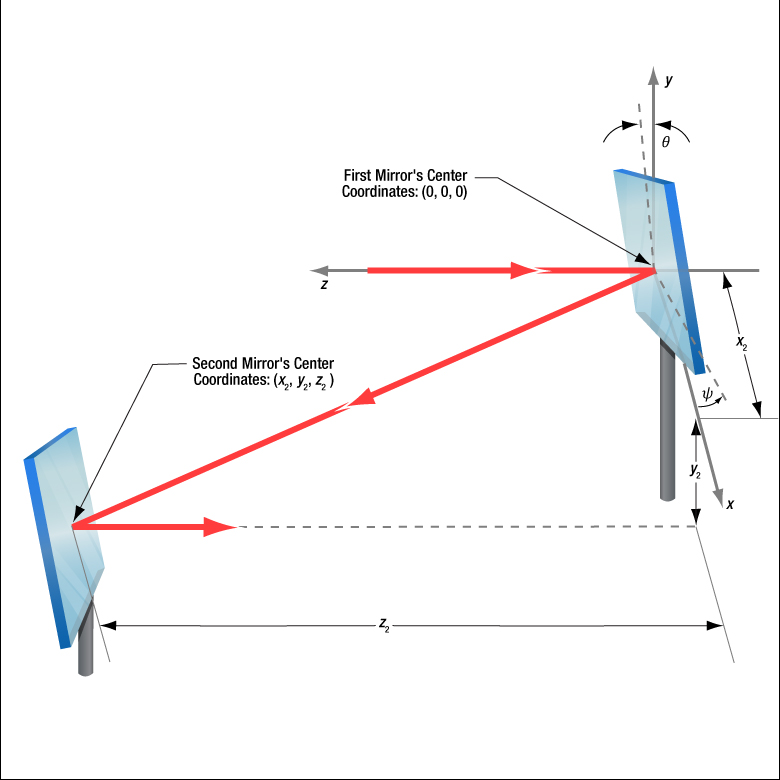
\includegraphics[width=3.8cm]{fig/twoMirror.jpg}
\end{center}
\end{column}
\end{columns}

\end{frame}


\begin{frame}\frametitle{Assignment: Two Mirror Walk}
\begin{columns}
\begin{column}{4cm}
\begin{center}
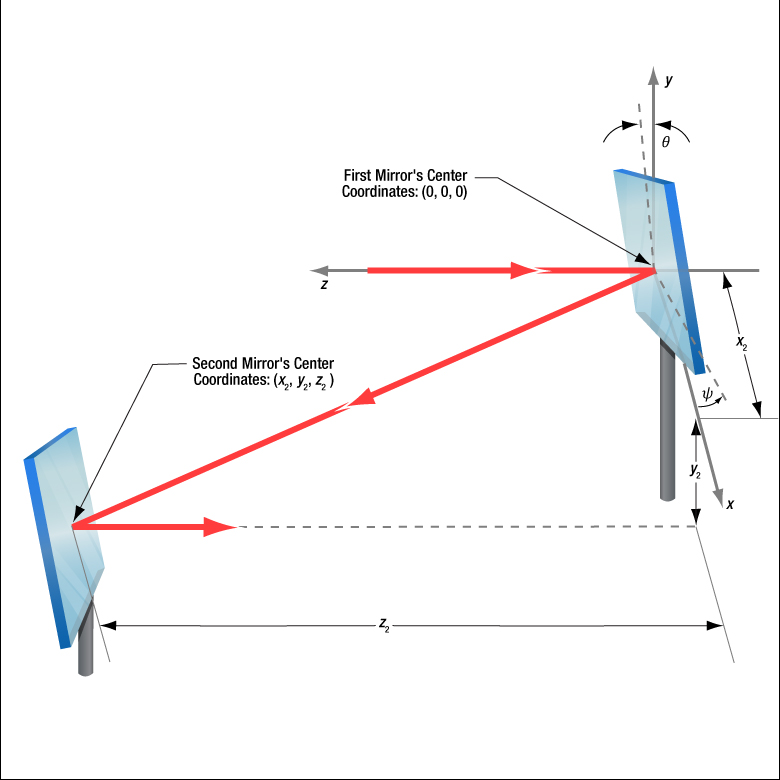
\includegraphics[width=3cm]{fig/twoMirror.jpg}

\vspace{1cm}
\includegraphics[width=4cm]{fig/twoMirror2.jpg}

\end{center}
\end{column}
\begin{column}{7.5cm}
\begin{itemize}
\item Supplies:
\begin{itemize}
\item Laser
\item Two mirrors set at different heights
\item Two irises, same height
\item Alignment target
\end{itemize}
\item Setup as shown on left
\item Adjust first mirror to hit center of second
\item Adjust second to shine laser through both iris
\end{itemize}
\end{column}
\end{columns}

\end{frame}

\section{Trigonometry}



\begin{frame}\frametitle{Algebraic Functions}
\begin{columns}
\begin{column}{4.5cm}
An algebraic function provides a "y-value" for every "x-value"
\begin{itemize}
\item Linear: $y = x + 2$
\item Quadratic: $y = x^2$
\item Periodic: $y = sin(x)$
\end{itemize}
\end{column}
\begin{column}{7cm}
\begin{center}
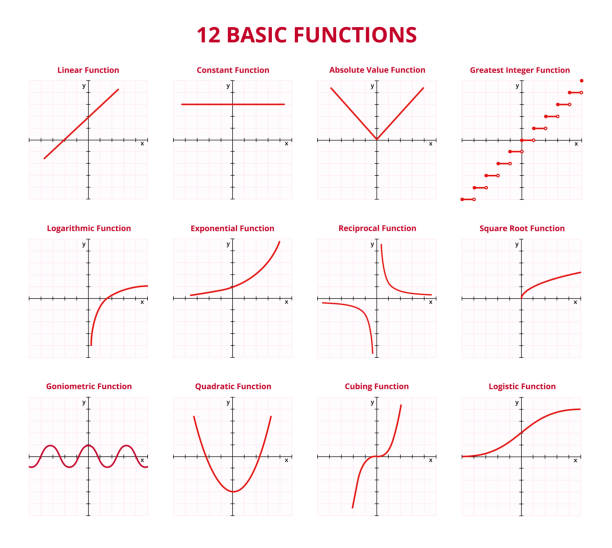
\includegraphics[width=7cm]{fig/basicfun.jpg}
\end{center}
\end{column}
\end{columns}
\end{frame}

\begin{frame}\frametitle{More Desmos Fun}

\begin{center}
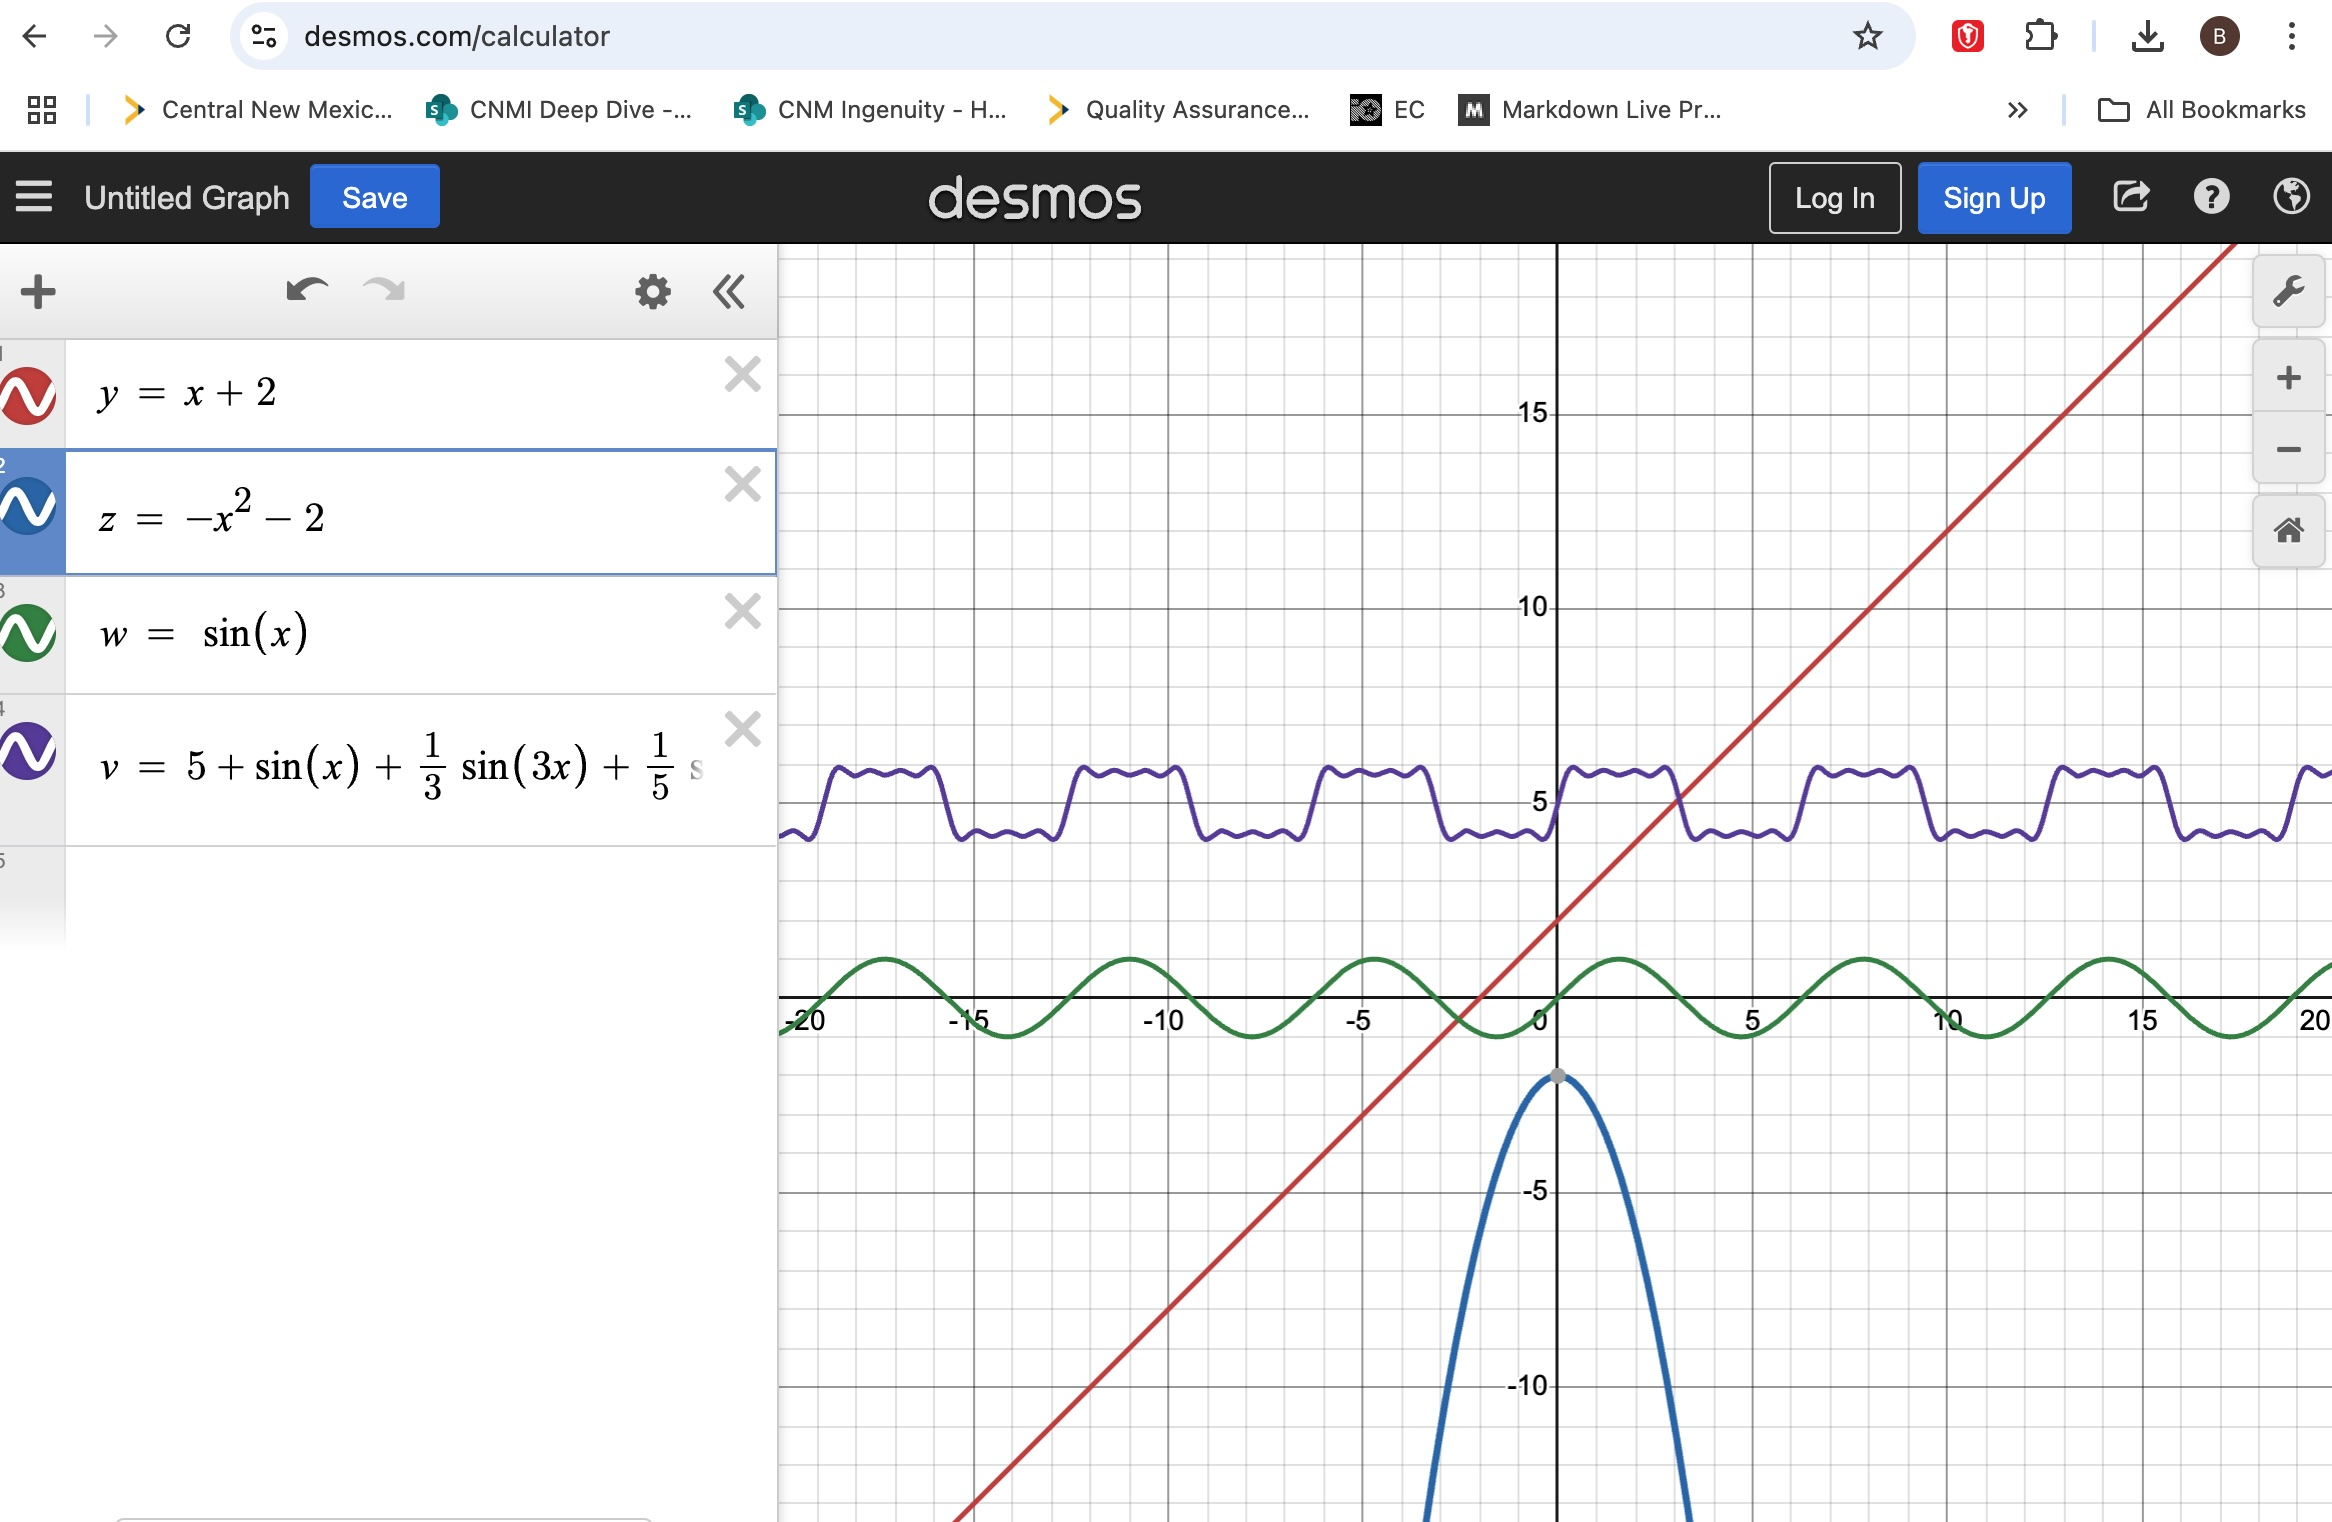
\includegraphics[width=12cm]{fig/desmosfun.jpg}
\end{center}
\end{frame}


\begin{frame}\frametitle{Pi ($\pi)$}

\begin{center}
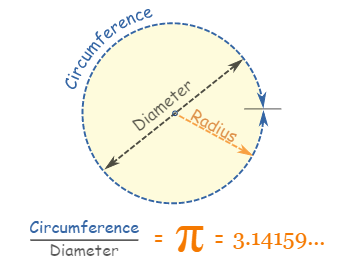
\includegraphics[width=8cm]{fig/pi.png}
\end{center}

\end{frame}


\begin{frame}\frametitle{Unit Circle and Trigonometric Functions}
The Unit Circle is a circle with a radius of 1.
\begin{columns}
\begin{column}{6cm}
\begin{center}
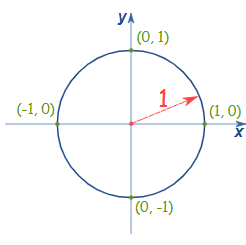
\includegraphics[scale=0.75]{fig/unitcircle.png}
\end{center}
\end{column}
\begin{column}{6cm}
\begin{center}
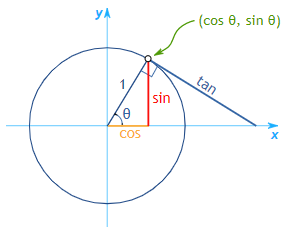
\includegraphics[scale=0.75]{fig/unitcircle_cst.png}
\end{center}
\end{column}
\end{columns}
The Unit Circle can be used to map out the trigonometric values of sine, cosine, and tangent.
\end{frame}


\begin{frame}\frametitle{Unit Circle and the Value of $sin(\theta)$}
\begin{columns}
\begin{column}{6cm}
\begin{center}
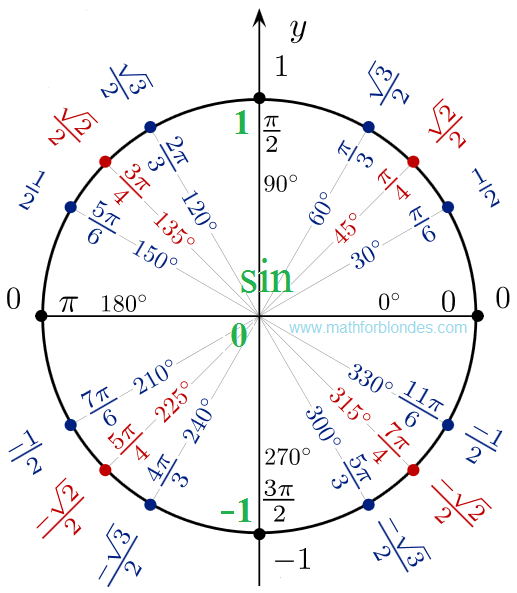
\includegraphics[scale=0.25]{fig/unitcircle_sin.png}
\end{center}
\end{column}
\begin{column}{6cm}
\begin{center}
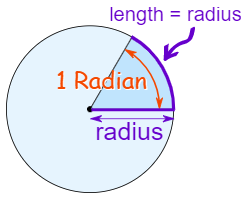
\includegraphics[scale=0.75]{fig/unitcircle_rad.png}
\end{center}
\end{column}
\end{columns}

\vspace{0.25cm}

\begin{itemize}
\item $sin(\theta)$ is the y-value of the point on the Unit Circle at angle $\theta$. 
\item In our trig functions, $\theta$ is measured in radians (rad), not degrees.
\item 360 degrees = $2 \pi$ radians.
\end{itemize}
\end{frame}



\begin{frame}\frametitle{Sine Waves}
\begin{center}
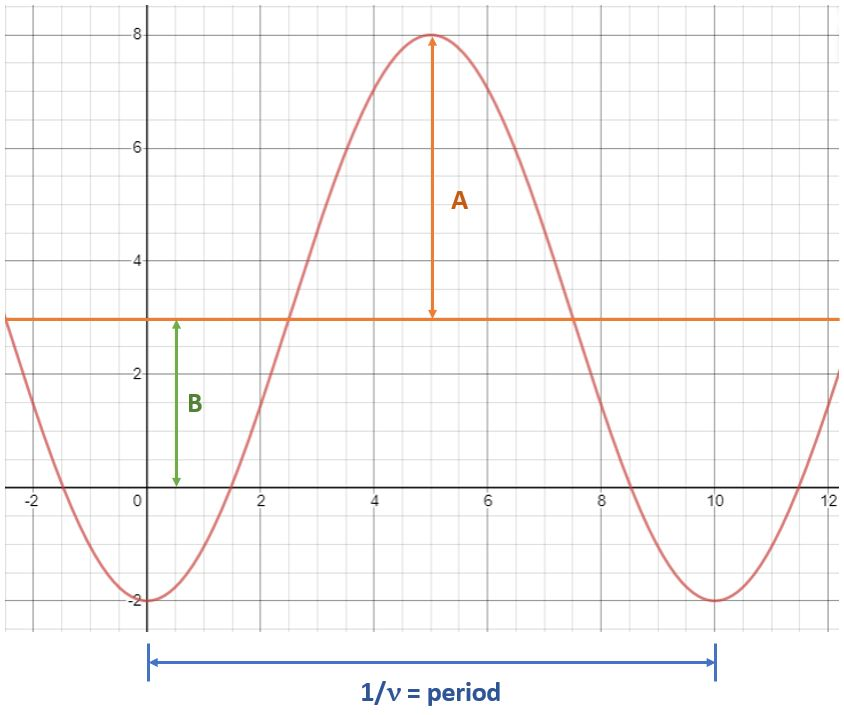
\includegraphics[scale=0.25]{fig/sin.jpg}
\end{center}

\begin{center}
$y = A * sin(2*\pi*\nu*t) + B$
\end{center}

where A = amplitude, B = offset, $\nu$ = frequency = $\frac{1}{period}$, 

and t = time in seconds.
\end{frame}


\begin{frame}\frametitle{Using Desmos (desmos.com/calculator)}
\begin{center}
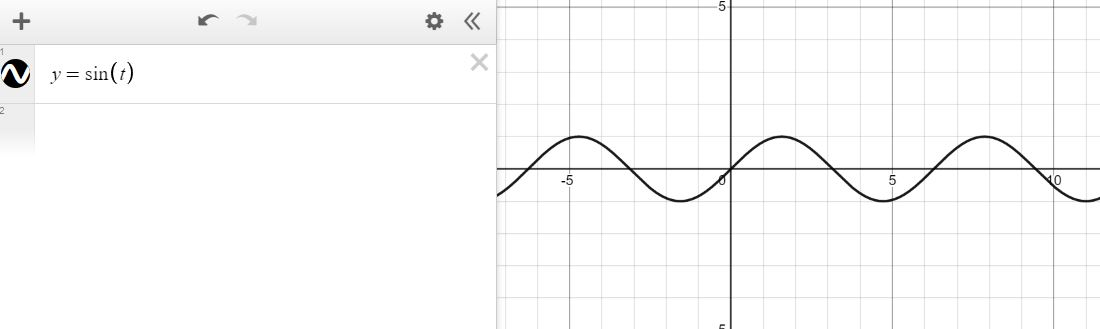
\includegraphics[scale=0.35]{fig/desmos1.jpg}
\end{center}
\begin{center}

\vspace{0.5cm}

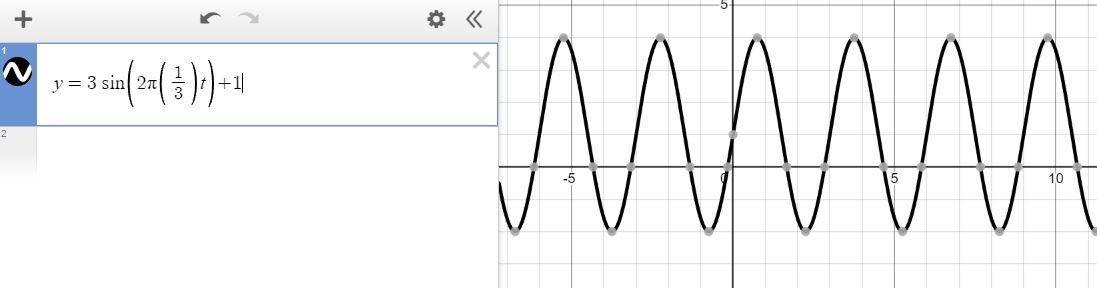
\includegraphics[scale=0.35]{fig/desmos2.jpg}
\end{center}
\end{frame}

\begin{frame}\frametitle{Phase Shift}
The sine wave can be shifted relative to each other by adding in a phase shift ($\phi$), which will shift the wave to the left or right.

Blue lags Red: 
\begin{center}
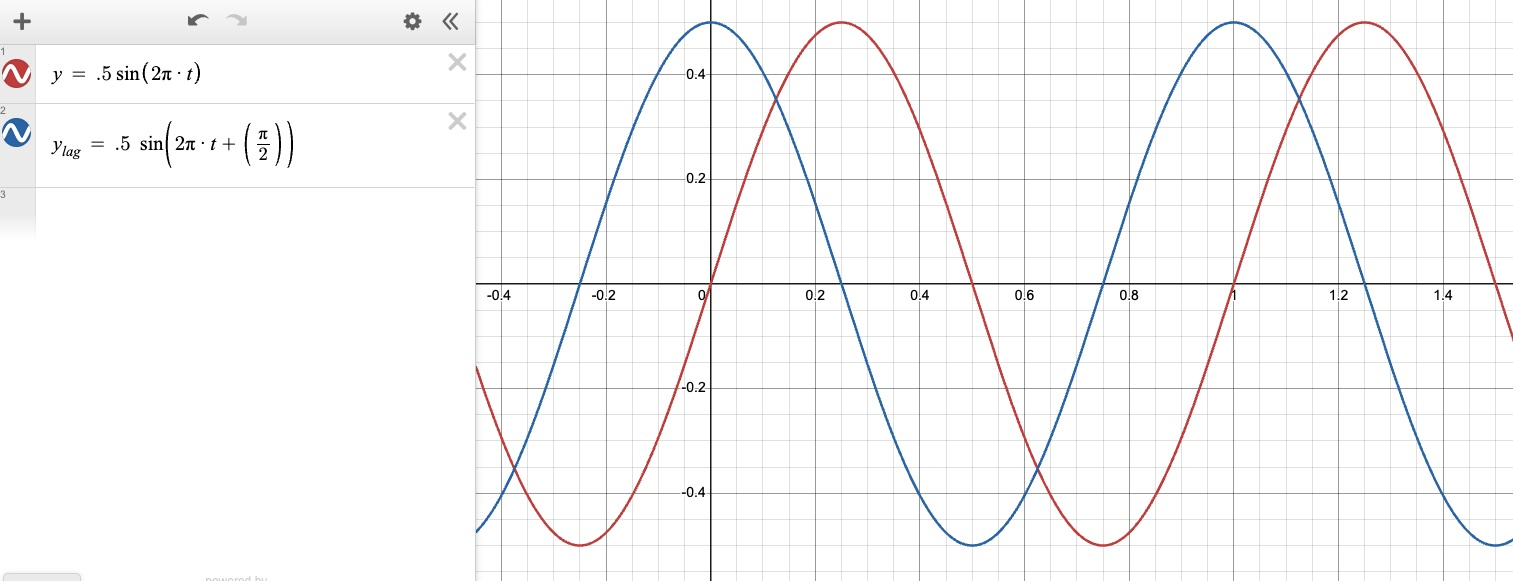
\includegraphics[height=2.6cm]{fig/sin_lag.jpg}
\end{center}

Green leads Red: 
\begin{center}
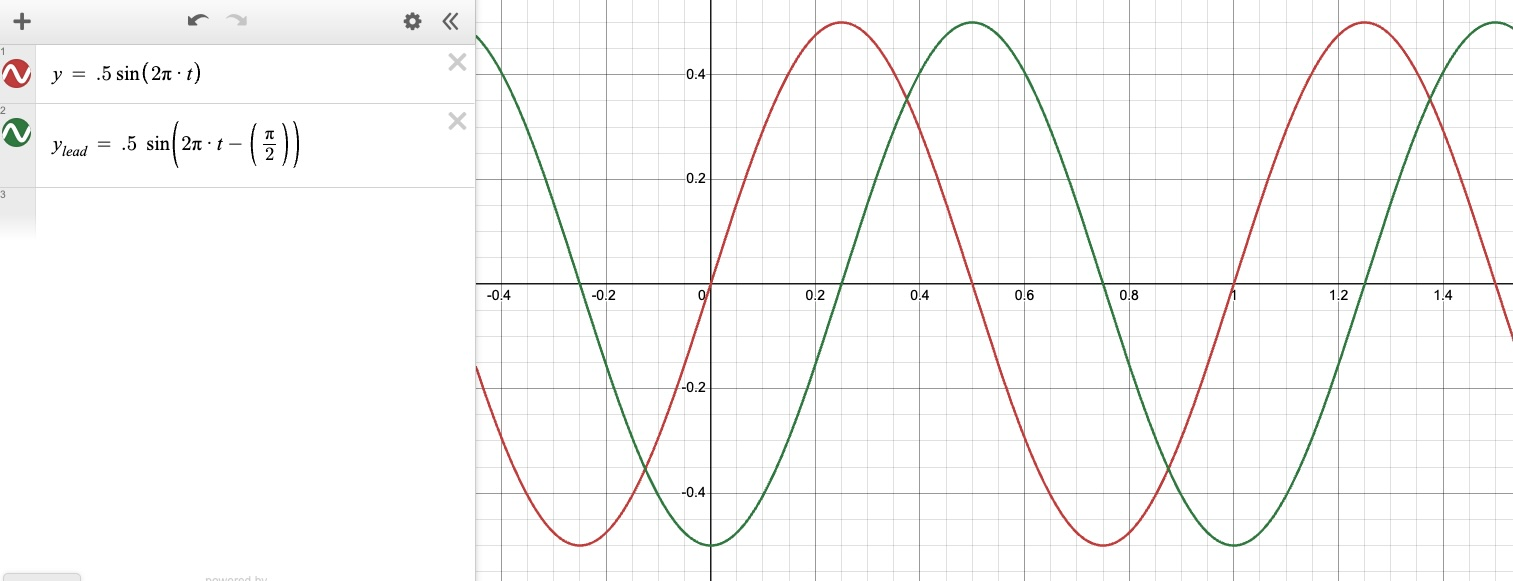
\includegraphics[height=2.6cm]{fig/sin_lead.jpg}
\end{center}

\end{frame}




\begin{frame}\frametitle{SOH CAH TOA}

\begin{itemize}
\item sin = opposite over hypotenuse
\item cos = adjacent over hypotenuse
\item tan = opposite over adjacent
\end{itemize}

\vspace{0.25cm}

\begin{center}
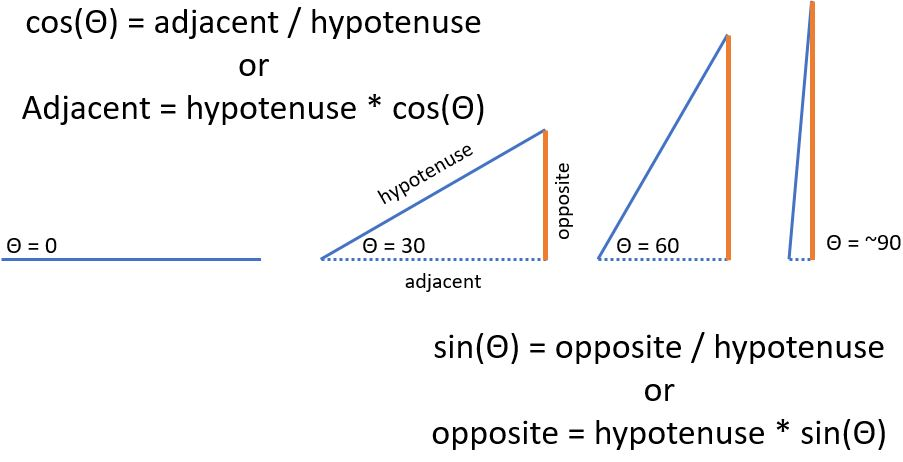
\includegraphics[scale=0.35]{fig/sohcahtoa.jpg}
\end{center}
\end{frame}

\begin{frame}\frametitle{Assignment: Calculating Angles}
\begin{columns}
\begin{column}{4cm}
\begin{center}
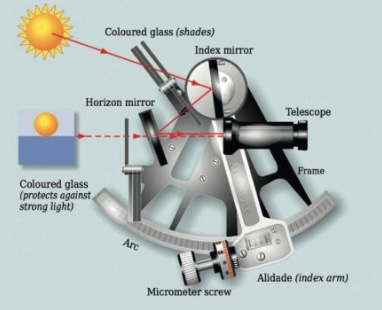
\includegraphics[width=4cm]{fig/sextant.jpg}
\end{center}
\end{column}
\begin{column}{7cm}
\begin{itemize}
\item Some assignment on measuring angles and using trig
\end{itemize}
\end{column}
\end{columns}
\end{frame}


\section{Return to Geometric Optics}

\begin{frame}\frametitle{Refraction}
The changing of a light ray’s direction (loosely called bending) when it passes through variations in matter is called refraction.

\begin{center}
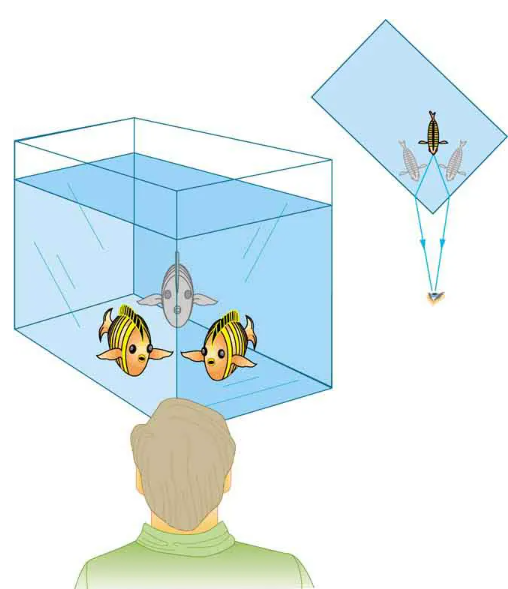
\includegraphics[width=5cm]{fig/fish.png}
\end{center}

\end{frame}


\begin{frame}\frametitle{Index of Refraction}

\begin{columns}
\begin{column}{6.5cm}
The speed of flight depends strongly on the type of material. We define the index of refraction ($n$) as

\begin{center}
$n = \frac{c}{v}$
\end{center}

where $v$ is the speed of light in the material and $c$ is the speed of light in a vacuum.
\end{column}
\begin{column}{5cm}
\begin{center}
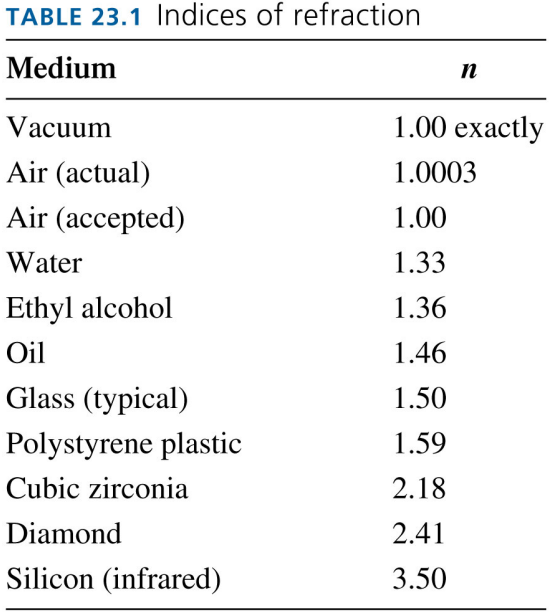
\includegraphics[width=5cm]{fig/n_table.png}
\end{center}
\end{column}
\end{columns}
\end{frame}

\begin{frame}\frametitle{Law of Refraction - Snell's Law}
The law of refraction is also called Snell’s law after the Dutch mathematician Willebrord Snell (1591–1626).

\begin{center}
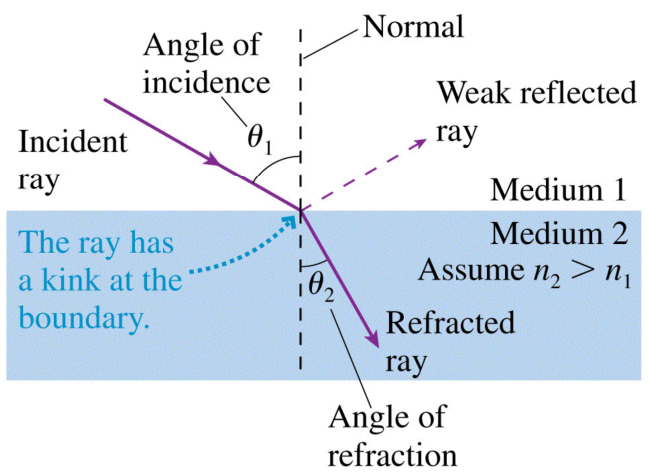
\includegraphics[width=6cm]{fig/snell.png}
\end{center}

\begin{center}
Snell's Law: $n_1 \sin{\theta_1} = n_2 \sin{\theta_2}$
\end{center}


\end{frame}

\begin{frame}\frametitle{Finding Index of Refraction}

Snells Law:

\begin{equation}
n_1 \sin{\theta_1} = n_2 \sin{\theta_2}
\end{equation}

Rearranging to isolate $n_2$:

\begin{equation}
n_2 = n_1 \frac{\sin{\theta_1}}{\sin{\theta_2}}
\end{equation}

For example, if the initial medium is air, $\theta_1 = 30^\circ \textdegree$ and $\theta_2 = 22^\circ$

\begin{equation}
n_2 = (1.00) \cdot \frac{\sin{30^\circ}}{\sin{22^\circ}} = \frac{0.500}{0.375} = 1.33
\end{equation}

\end{frame}

\begin{frame}\frametitle{Assignment: Measuring Refraction}
\begin{columns}
\begin{column}{4cm}
\begin{center}
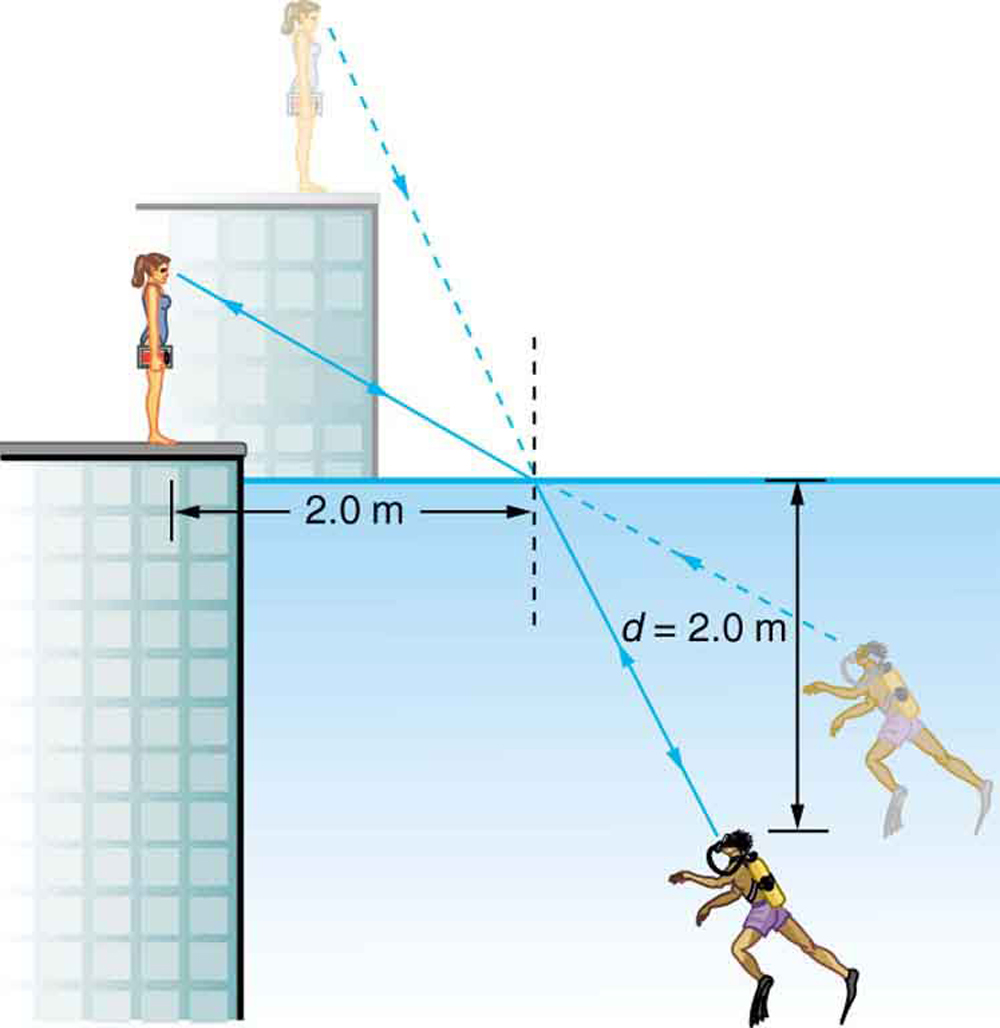
\includegraphics[width=4cm]{fig/refract9.jpg}
\end{center}
\end{column}
\begin{column}{7cm}
\begin{itemize}
\item Some assignment on refraction
\item Acrylic, water, what else?
\item Different color lasers (red, green, and if we get blue in time)
\end{itemize}
\end{column}
\end{columns}
\end{frame}


\begin{frame}\frametitle{Total Internal Reflection}

\begin{columns}
\begin{column}{9.5cm}
Good mirrors reflect $>90$\% of the light; however, total reflection can be produced via refraction.\newline

If the index of refraction of the second medium is less than that of the first medium, the rays are refracted away from the perpendicular. 

\begin{itemize}
\item Since $n_1 > n_2$, the angle of refraction is greater than the angel of incidence: $\theta_2 > \theta_1$.
\item Increasing $\theta_1$ causes $\theta_2$ to increase.
\item The critical angle ($\theta_c$) is defined to be the incident angle ($\theta_1$) that produces a $\theta_2 = 90^\circ$ 
\end{itemize}

The critical angle is given by:
\begin{equation}
\theta_c = sin^{-1}(\frac{n_2}{n_1}), \hspace{3mm} \text{for} \hspace{2mm}  n_1 > n_2
\end{equation}

\end{column}
\begin{column}{3cm}
\begin{center}

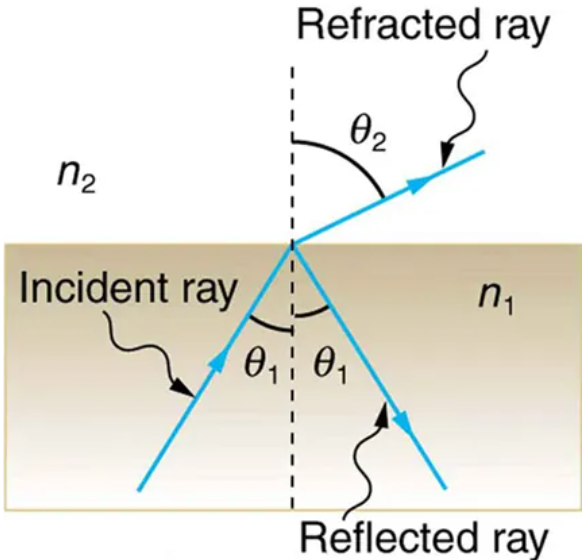
\includegraphics[width=2.5cm]{fig/tir1.png}

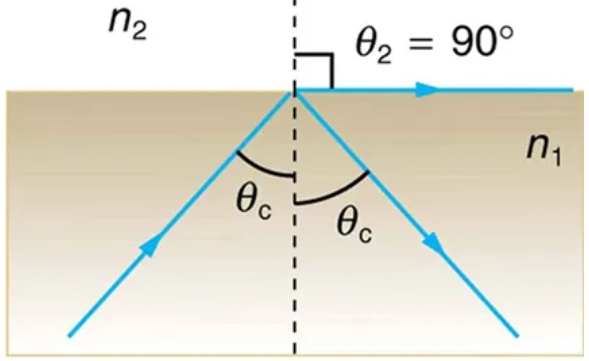
\includegraphics[width=2.5cm]{fig/tir2.png}

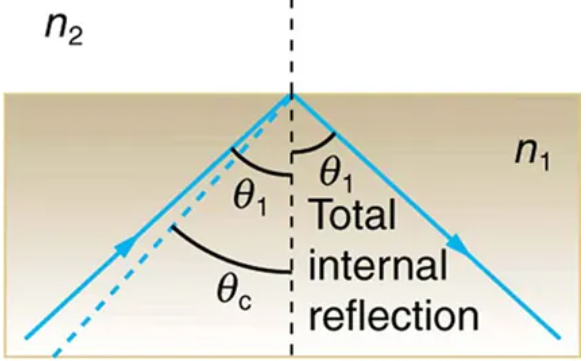
\includegraphics[width=2.5cm]{fig/tir3.png}

\end{center}
\end{column}
\end{columns}
\end{frame}


\begin{frame}\frametitle{Fiber Optic Cable}
The fiber optic cable takes advantage of the core having a high index of refraction than the cladding.

\begin{center}
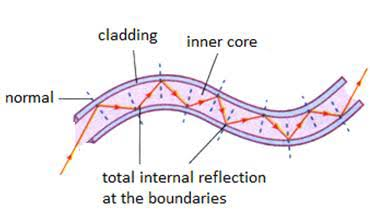
\includegraphics[width=6cm]{fig/cladding.jpg}
\end{center}

\vspace{3cm}

More to come on fibers as we progress through the Quantum Journey


\end{frame}



\begin{frame}\frametitle{Fiber: Acceptance Angle}
For multi-mode fibers, the numerical appeture (NA) provides  a good estimate of the maximum acceptance angle. 
\begin{columns}
\begin{column}{7cm}


\begin{itemize}
\item The cutoff angle is the maximum acceptance angle ($\theta_{max}$), which is related to NA:
\[ NA = n_0 sin(\theta_{max}) = \sqrt{n_{core}^2 + n_{clad}^2} \]

\item Rays with an angle of incidence $\leq \theta_{max}$ are totally internally reflected (TIR) at the fiber core/cladding boundary.

\item Rays with an angle of incidence $> \theta_{max}$ refract at and pass through the boundary.

\end{itemize}

\end{column}
\begin{column}{4cm}
\begin{center}

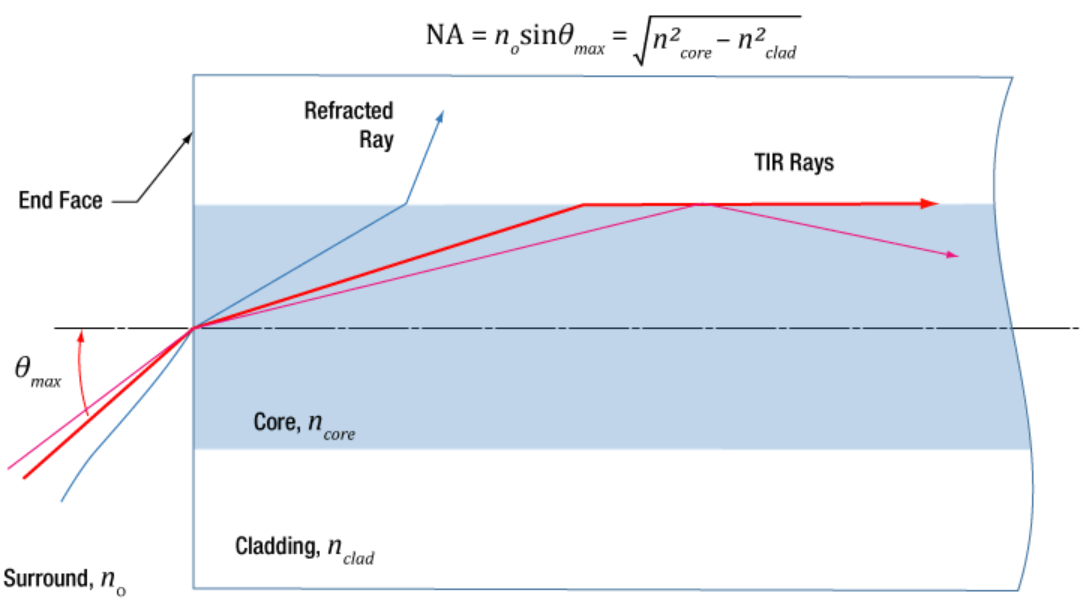
\includegraphics[width=3.8cm]{fig/fiber_NA.png}

\vspace{0.25cm}

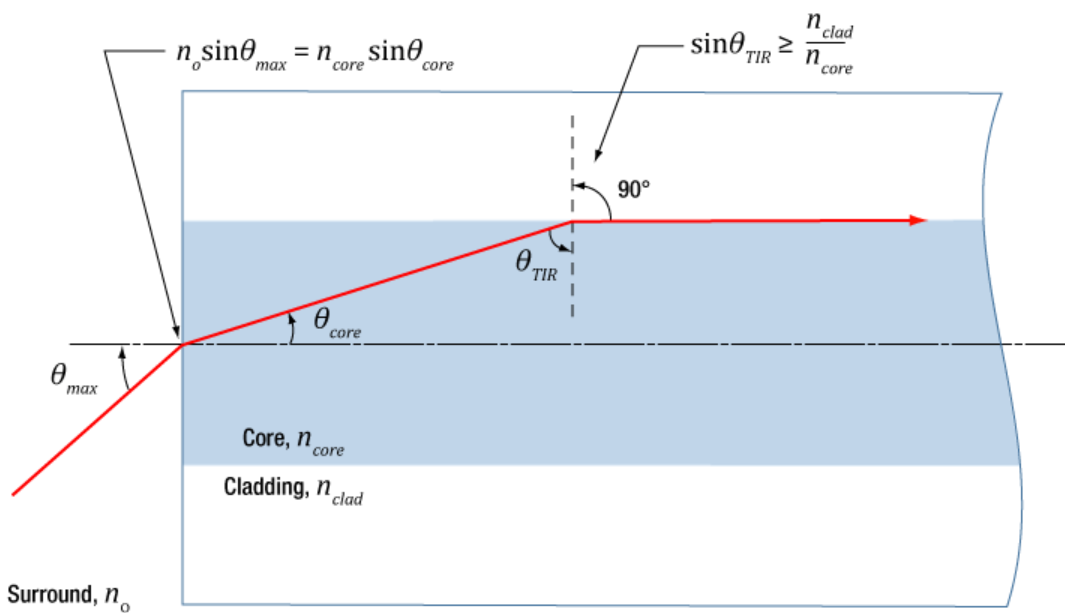
\includegraphics[width=3.8cm]{fig/fiber_TIR.png}

\end{center}
\end{column}
\end{columns}
\end{frame}


\begin{frame}\frametitle{Dispersion}
Dispersion is defined to be the spreading of white light into its full spectrum of wavelengths.

\begin{center}
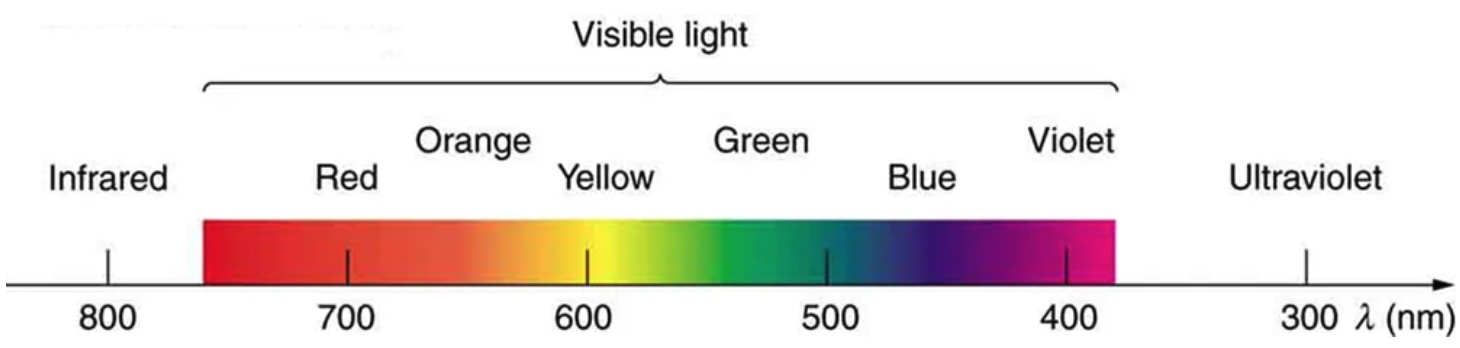
\includegraphics[width=10cm]{fig/rainbow.jpg}
\end{center}

\begin{itemize}
\item The angle of refraction depends on the index of refraction.
\item The index of refraction (n) depends on the properties of the medium.
\item However, for a given medium, n also depends on the optical wavelength.
\end{itemize}


\end{frame}

\begin{frame}\frametitle{Index of Refraction by Wavelength}
Index of refraction ($n$) by wavelength ($\lambda$):

\begin{center}
\includegraphics[width=10cm]{fig/nbylambda.jpg}
\end{center}
\end{frame}


\begin{frame}\frametitle{Glass Prism}
\begin{columns}
\begin{column}{5.5cm}
\begin{center}
\includegraphics[height=3.6cm]{fig/gpideal.jpg}
\end{center}
\end{column}
\begin{column}{5.5cm}
\begin{center}
\includegraphics[height=3.7cm]{fig/gpreal.jpg}
\end{center}
\end{column}
\end{columns}
\end{frame}

\begin{frame}\frametitle{Rainbow}
\begin{center}
\includegraphics[width=6cm]{fig/rainbow2.jpg}
\end{center}
Rainbows are produced by a combination of refraction and reflection. You may have noticed that you see a rainbow only when you look away from the sun. Light enters a drop of water and is reflected from the back of the drop. The light is refracted both as it enters and as it leaves the drop. Since the index of refraction of water varies with wavelength, the light is dispersed, and a rainbow is observed.
\end{frame}

\begin{frame}\frametitle{Rainbow as an Arc}
\begin{columns}
\begin{column}{5.5cm}
\begin{center}
\includegraphics[width=5cm]{fig/rainbow3.jpg}
\end{center}
\end{column}
\begin{column}{5.5cm}
\begin{center}
\includegraphics[width=5cm]{fig/rainbow4.jpg}
\end{center}
\end{column}
\end{columns}
\end{frame}


\section{Lens}

\begin{frame}\frametitle{Lens}
With the Law of Refraction, we can explore the properties of lens and how images are formed.
\begin{columns}
\begin{column}{6.5cm}
\begin{itemize}
\item The word lens comes from the Latin word for lentil bean, the shape of which is similar to a convex lens.
\item Convex Lens: all light rays that enter parallel to the axis cross one another at  a single point on the opposite side of the lens, i.e., they converge.
\item Concave Lens: all light rays that enter parallel to the axis diverge (bend away) from the lens axis.
\end{itemize}
\end{column}
\begin{column}{4.5cm}
\begin{center}
\includegraphics[width=4cm]{fig/cavevex.jpg}
\end{center}
\end{column}
\end{columns}
\end{frame}


\begin{frame}\frametitle{Convex Lens}
With the Law of Refraction, we can explore the properties of lens and how images are formed.
\begin{columns}
\begin{column}{6cm}
\begin{itemize}
\item A ray of light bends (refracts) at both interface, and for convex lens converge.
\item The point at which the rays crossed is defined as the Focal point ($F$) of the lens.
\item The distance from the center of the lens to its focal point is called the focal length ($f$).
\item The Power of the lens, measuring in Diopters ($P=\frac{1}{f}$) where $f$ is measured in meters.
\end{itemize}
\end{column}
\begin{column}{5cm}
\begin{center}
\includegraphics[width=4cm]{fig/convex1.jpg}

\vspace{0.25cm}
\includegraphics[width=4cm]{fig/convex2.jpg}
\end{center}
\end{column}
\end{columns}
\end{frame}

\begin{frame}\frametitle{Concave Lens}
\begin{columns}
\begin{column}{6cm}
\begin{itemize}
\item A concave lens is a diverging lens, it causes light rays to bend away from the axis.
\item In the case of all rays entering parallel to its axis, the light appears to originate at the same point $F$.
\item The distance from the center of the lens to its focal point is called the focal length ($f$) and is defined to be negative.
\end{itemize}
\end{column}
\begin{column}{5cm}
\begin{center}
\includegraphics[width=4cm]{fig/concave1.jpg}

\vspace{0.25cm}
\includegraphics[width=4cm]{fig/concave2.jpg}
\end{center}
\end{column}
\end{columns}
\end{frame}

\begin{frame}\frametitle{Thin Lens}
A thin lens is defined to be one whose thickness allows rays to refract but does not allow properties such as dispersion and aberrations.
\end{frame}

\begin{frame}\frametitle{Ray Tracing}
\begin{columns}
\begin{column}{7.4cm}
\begin{enumerate}
\item A ray entering a converging lens parallel to its axis passes through the focal point F of the lens on the other side.
\item A ray entering a diverging lens parallel to its axis seems to come from the focal point F.
\item A ray passing through the center of either a converging or a diverging lens does not change direction.
\item A ray entering a converging lens through its focal point exits parallel to its axis.
\item A ray that enters a diverging lens by heading toward the focal point on the opposite side exits parallel to the axis.
\end{enumerate}


\end{column}
\begin{column}{4.6cm}
\begin{center}
\includegraphics[width=4.5cm]{fig/raytrace.jpg}
\end{center}
\end{column}
\end{columns}
\end{frame}


\begin{frame}\frametitle{Image Formation}

\begin{center}
\includegraphics[width=8cm]{fig/imageform1.jpg}
\end{center}


Thin Lens equations:

\begin{columns}
\begin{column}{5.5cm}
\[ \frac{1}{d_o} + \frac{1}{d_i} = \frac{1}{f}\]
\end{column}
\begin{column}{5.5cm}
\[ \frac{h_i}{h_o} = -\frac{d_i}{d_o} = m\]
\end{column}
\end{columns}

\end{frame}


\begin{frame}\frametitle{Image Formation - Real Image}
\begin{columns}
\begin{column}{5.5cm}
\begin{center}
\includegraphics[width=5cm]{fig/imageform2.jpg}
\end{center}
\end{column}
\begin{column}{5.5cm}
\begin{center}
\includegraphics[width=5cm]{fig/imageform3.jpg}
\end{center}
\end{column}
\end{columns}

\vspace{1cm}

The image in which light rays from one point on the object actually cross at the location of the image and can be projected onto a screen, a piece of film, or the retina of an eye is called a real image.

\end{frame}

\begin{frame}\frametitle{Image Formation - Virtual Image}

\begin{center}
\includegraphics[width=8cm]{fig/imageform4.jpg}
\end{center}

If an object is held closer to the converging lens than its focal length ($f$), then the rays from a common point continue to diverge after passing through the lens. They all appear to originate from a point at the location of the image, on the same side of the lens as the object. This is a virtual image. 


\end{frame}

\begin{frame}\frametitle{Image Formation - Concave Lens}

\begin{center}
\includegraphics[width=8cm]{fig/imageform5.jpg}
\end{center}
\end{frame}


\begin{frame}\frametitle{Beam Expander/Reducer - Telescope}
\begin{columns}
\begin{column}{5.5cm}
\begin{center}
\includegraphics[width=5cm]{fig/beamXkepler.png}
Galilean Design
\end{center}
\end{column}
\begin{column}{5.5cm}
\begin{center}
\includegraphics[width=5cm]{fig/beamXgalileo.png}
Galilean Design
\end{center}
\end{column}
\end{columns}

\vspace{0.25cm}
Both the bean's waist ($2W_0$) and the divergence angle ($\theta$) are affected by by the beam expanders and reducers. If Lens 2 is the output lens, then the beam expansion ratio ($m_{12}$) is: 
\begin{equation}
m_{12} = \frac{f_2}{f_1}
\end{equation}

\end{frame}

\subsection{mirrors}

\begin{frame}\frametitle{Flat Mirror}

\begin{center}
\includegraphics[width=10cm]{fig/mirrorimage1.jpg}
\end{center}

\end{frame}

\begin{frame}\frametitle{Concave Spherical Mirrors - Thin Lens Equivalent}

\begin{center}
\includegraphics[width=10cm]{fig/mirrorimage2.jpg}
\end{center}

For a mirror that is large compared to the radius of curvature, the reflected rays do not cross at the same point. A parabolic mirror, the rays would indeed cross at a single point. However, parabolic mirrors are expensive. So, using a mirror that is small compared to the radius of curvature, leads to a well-defined focal point $F$, with $f = \frac{R}{2}$.

\end{frame}

\begin{frame}\frametitle{Convex Mirrors}

\begin{center}
\includegraphics[width=5cm]{fig/mirrorimage3.jpg}
\end{center}

\end{frame}

\begin{frame}\frametitle{Image Formation - Concave Mirrors}

\begin{center}
\includegraphics[width=8cm]{fig/mirrorimage4.jpg}
\end{center}

\end{frame}

\begin{frame}\frametitle{Image Formation - Concave Mirrors}

\begin{center}
\includegraphics[width=8cm]{fig/mirrorimage5.jpg}
\end{center}

\end{frame}

\begin{frame}\frametitle{Image Formation - Convex Mirrors}

\begin{center}
\includegraphics[width=8cm]{fig/mirrorimage6.jpg}
\end{center}

\end{frame}

\section{Vision}

\begin{frame}\frametitle{The Eye}

\begin{center}
\includegraphics[width=6cm]{fig/theI.jpg}
\end{center}

\end{frame}

\begin{frame}\frametitle{Rods and Cones and Color}

\begin{center}
\includegraphics[width=6cm]{fig/rodscones.jpg}
\end{center}

\end{frame}

\begin{frame}\frametitle{Visible Spectrum}

\begin{center}
\includegraphics[width=10cm]{fig/visSpec.jpg}
\end{center}

\end{frame}

\begin{frame}\frametitle{Spectrum of Light Sources}

\begin{center}
\includegraphics[width=10cm]{fig/lightSpec.jpg}
\end{center}

\end{frame}

\begin{frame}\frametitle{Chromatic Aberrations}

\begin{center}
\includegraphics[width=10cm]{fig/chromeAbb.jpg}
\end{center}

\end{frame}

\begin{frame}\frametitle{Correcting Chromatic Aberrations}

\begin{center}
\includegraphics[width=10cm]{fig/chromeAbb2.jpg}
\end{center}

\end{frame}

\begin{frame}\frametitle{Coma - Off Axis Abberation}

\begin{center}
\includegraphics[width=10cm]{fig/coma.jpg}
\end{center}

\end{frame}

\begin{frame}\frametitle{Spherical Aberrations}

\begin{center}
\includegraphics[width=10cm]{fig/sphereAbb.jpg}
\end{center}

\end{frame}



\section{Interlude: Light - a particle or a wave?}

\begin{frame}\frametitle{Corpuscular Theory of Light}

In 1675, Sir Isaac Newton hypothesized that light was made up corpuscules (small particles) with the size/mass of the corresponding to different colors. 

\begin{columns}
\begin{column}{3.5cm}
\begin{center}
\includegraphics[width=3cm]{fig/corpReflect.png}
\end{center}
\end{column}

\begin{column}{3.5cm}
\begin{center}
\includegraphics[width=3cm]{fig/corpRefract.png}
\end{center}
\end{column}

\begin{column}{3.5cm}
\begin{center}
\includegraphics[width=3cm]{fig/corpDoubleSlit.png}
\end{center}
\end{column}
\end{columns}
\end{frame}

\begin{frame}\frametitle{Huygens Principle}
\begin{columns}
\begin{column}{3cm}
\begin{center}
\includegraphics[width=2cm]{fig/grimaldi.png}

\vspace{0.5cm}

\includegraphics[width=2cm]{fig/huygens.png}

\end{center}
\end{column}

\begin{column}{8cm}
\begin{itemize}
\item Francesco Maria Grimaldi (mid-1600's) made accurate observations of the diffraction of light.

\vspace{0.5cm}

\item In 1678, Christian Huygens, in order to explain the diffraction of light, proposed that every point on a wavefront (of light) is a wavelet that spreads.
\end{itemize}
\end{column}
\end{columns}

\end{frame}


\begin{frame}\frametitle{Fresnel and Young}
\begin{columns}
\begin{column}{3cm}
\begin{center}
\includegraphics[width=3cm]{fig/fresnel.png}

\vspace{0.5cm}

\includegraphics[width=3cm]{fig/youngDoubleSlit.jpg}

\end{center}
\end{column}

\begin{column}{8cm}
\begin{itemize}
\item In 1815, Augistine Jean Fresnel devleoped the laws of reflection and refraction.

\vspace{0.5cm}

\item And, in 1817, Thomas Young calculated the wavelength of light
\end{itemize}
\end{column}
\end{columns}

\end{frame}

\begin{frame}\frametitle{Maxwell's Equations: Electric $\vec{E}$ and Magnetic $\vec{B}$ Fields}
In 1864, James Clerk Maxwell predicted electromagnetic waves
\begin{itemize}
\item Gauss's Law: $\nabla \cdot \vec{E} = \frac{\rho}{\epsilon_0}$, where ${\rho}$ is enclosed charge
\item Guass's Law for Magnets: $\nabla \cdot \vec{B} = 0$
\item Farday's Law: $\nabla \times \vec{E} = -\frac{\partial \vec{B}}{\partial t}$
\item Ampere's Law: $\nabla \times \vec{B} = \mu_0 \vec{J} + \mu_0 \epsilon_0 \frac{\partial \vec{E}}{\partial t}$
\end{itemize}

where \newline
$\mu_0 = 4 \pi*10^{-7} \frac{F}{m}$ and 
$\epsilon_0 = 8.85*10^{-12} \frac{N m^2}{C}$ \newline

Maxwell noted that the speed of the electromagnetic wave is equal to the speed of light:


$\frac{1}{\sqrt{\mu_0 \epsilon_0}}= \frac{1}{\sqrt{4 \pi*10^{-7} \cdot 8.85*10^{-12}}} = 2.99*10^{8} \frac{m}{s} = c$
\end{frame}

\section{Wave Optics}

\begin{frame}\frametitle{Speed of Light in a Medium}
The speed of a wave is the frequency ($\frac{1}{s}$) times the wavelength ($m$):
\begin{equation}
c = f \lambda
\end{equation}
where in a vacuum, $c = 2.99 * 10^8 (\frac{m}{s})$. \newline

Light has wave characteristics in a medium other than a vacuum, as well. In this case, the speed and wavelength change, but the frequency stays the same. The speed of light in a medium is governed by its index of refraction ($n$), where $v = \frac{c}{n}$. \newline

Divide both sides of the above equation by $n$ yields:
\begin{equation}
v = \frac{c}{n} = \frac{f \lambda}{n} = f \lambda_n
\end{equation}
where $\lambda_n$ is the wavelength in the medium.
\end{frame}

\begin{frame}\frametitle{Huygens's Principle: Diffraction}
\begin{columns}
\begin{column}{7cm}
Every point on a wavefront is a source of wavelets that spread out in the forward direction at the same speed as the wave itself. The new wavefront is a line tangent to all of the wavelets.
\end{column}
\begin{column}{4cm}
\begin{center}
\includegraphics[width=3cm]{fig/huygens.jpg}
\end{center}
\end{column}
\end{columns}
\end{frame}

\begin{frame}\frametitle{Huygens's Mirror}
\begin{columns}
\begin{column}{6cm}
A mirror reflects an incoming wave at an angle equal to the incident angle, verifying the law of reflection. As the wavefront strikes the mirror, wavelets are first emitted from the left part of the mirror and then the right. The wavelets closer to the left have had time to travel farther, producing a wavefront traveling in the direction shown.
\end{column}
\begin{column}{5cm}
\begin{center}
\includegraphics[width=5cm]{fig/huyMirror.jpg}
\end{center}
\end{column}
\end{columns}
\end{frame}

\begin{frame}\frametitle{Huygens's Refraction}
\begin{columns}
\begin{column}{6cm}
Each wavelet to the right was emitted when the wavefront crossed the interface between the media. Since the speed of light is slower in the second medium, the waves do not travel as far in a given time, and the new wavefront changes direction as shown. This explains why a ray changes direction to become closer to the perpendicular when light slows down and can be used to derive Snell's Law.
\end{column}
\begin{column}{5cm}
\begin{center}
\includegraphics[width=5cm]{fig/huyRefract.jpg}
\end{center}
\end{column}
\end{columns}
\end{frame}

\begin{frame}\frametitle{Diffraction}
\begin{columns}
\begin{column}{6cm}
While the ray optics method is useful, if light indeed traveled in straight rays then there would be a pitch black shadow where the light is blocked by the wall.
\end{column}
\begin{column}{5cm}
\begin{center}
\includegraphics[width=5cm]{fig/doorway.jpg}
\end{center}
\end{column}
\end{columns}
\end{frame}

\begin{frame}\frametitle{Diffraction}
\begin{center}
\includegraphics[width=8cm]{fig/diffraction.jpg}
\end{center}

If we pass light through smaller openings, often called slits, we can use Huygens’s principle to see that light bends. The bending of a wave around the edges of an opening or an obstacle is called diffraction. Diffraction is a wave characteristic and occurs for all types of waves.
\end{frame}

\begin{frame}\frametitle{Constructive Interference}
\begin{center}
\includegraphics[width=8cm]{fig/constructive.jpg}
\end{center}


\end{frame}


\begin{frame}\frametitle{Destructive Interference}
\begin{center}
\includegraphics[width=8cm]{fig/destructive.jpg}
\end{center}
\end{frame}

\begin{frame}\frametitle{Double Slit}
\begin{center}
\includegraphics[width=6cm]{fig/ds1.jpg}
\includegraphics[width=6cm]{fig/ds2.jpg}
\end{center}

\end{frame}


\begin{frame}\frametitle{Path Length Difference}
\begin{columns}
\begin{column}{7cm}
\begin{itemize}
\item Constructive Interference - peaks are in phase
\[d \sin{(\theta}) = m \lambda, m = 0,1,-1,2,-2,....\]
\item Destructive Interference - peaks are perfectly out of phase
\[d \sin{(\theta}) = (m+\frac{1}{2})  \lambda, m = 0,1,-1,2,-2,....\]
\end{itemize}
\end{column}
\begin{column}{4cm}
\begin{center}
\includegraphics[width=4cm]{fig/ds3.jpg}
\end{center}
\end{column}
\end{columns}
\end{frame}

\begin{frame}\frametitle{Double Slit - Constructive Interference}
\begin{center}
\includegraphics[width=8cm]{fig/ds4.jpg}
\end{center}

\end{frame}


\begin{frame}\frametitle{Diffraction Grating}
\begin{columns}
\begin{column}{5cm}
If light is passed through a large number of evenly spaced parallel slits, called a diffraction grating, the interference pattern is created that is very similar to the one formed by a double slit. \newline

Diffraction gratings can be made to work with the transmission or reflection of light. 
\end{column}
\begin{column}{6cm}
\begin{center}
\includegraphics[width=5.8cm]{fig/dg1.jpg}
\end{center}
\end{column}
\end{columns}
\end{frame}


\begin{frame}\frametitle{Diffraction Grating - Constructive Interference}
\begin{columns}
\begin{column}{7cm}
Similar to a double slit, the constructive interference happens on integral number of wavelengths:

\[d \cdot sin(\theta) = m \lambda \]

for, $m = 0, 1 , -1, 2, -2, ...$


\end{column}
\begin{column}{4cm}
\begin{center}
\includegraphics[width=3.8cm]{fig/dg2.jpg}
\end{center}
\end{column}
\end{columns}
\end{frame}

\begin{frame}\frametitle{Diffraction Grating - Spread of Wavelength}
\begin{columns}
\begin{column}{7cm}
We can find $\theta_R$, $y_R$, $\theta_V$, and $y_V$ by using:

\[d \cdot sin(\theta) = m \lambda \]

for, $m = 1$.


\end{column}
\begin{column}{4cm}
\begin{center}
\includegraphics[width=3.8cm]{fig/dg3.jpg}
\end{center}
\end{column}
\end{columns}
\end{frame}


\begin{frame}\frametitle{Single Slit}
\begin{columns}
\begin{column}{5cm}
\begin{center}
\includegraphics[height=7cm]{fig/sl2.jpg}
\end{center}


\end{column}
\begin{column}{6cm}
\begin{center}
\includegraphics[width=4cm]{fig/sl1.jpg}

\includegraphics[width=4cm]{fig/sl3.jpg}
\end{center}
\end{column}
\end{columns}
\end{frame}


\begin{frame}\frametitle{Limits of Resolution}

Diffraction affects the detail that can be observed when light passes through an aperture.

\vspace{0.5cm}

\begin{center}
\includegraphics[width=10cm]{fig/rayleigh1.jpg}
\end{center}

\end{frame}

\begin{frame}\frametitle{Limits of Resolution}

Diffraction affects the detail that can be observed when light passes through an aperture.

\vspace{0.5cm}

\begin{center}
\includegraphics[width=10cm]{fig/rayleigh1.jpg}
\end{center}

\end{frame}


\begin{frame}\frametitle{Rayleigh Criterion}


Two points are just resolved if they are separated by an angle of $\theta = 1.22 \frac{\lambda}{D}$

\vspace{0.25cm}

\begin{center}
\includegraphics[width=8cm]{fig/rayleigh2.jpg}
\end{center}
\end{frame}

\begin{frame}\frametitle{Resolving Power}
\begin{columns}
\begin{column}{7cm}
The resolving power of a system is the smallest distance of separation ($x$) where two objects can be seen as distinct. It is given by the Rayleigh Criterion:

\[\theta = 1.22 \cdot \frac{\lambda}{D} = \frac{x}{d}\]
where $d$ is the between the lens objective and the object.

\end{column}
\begin{column}{4cm}
\begin{center}
\includegraphics[width=3cm]{fig/rayleigh3.jpg}
\end{center}
\end{column}
\end{columns}
\end{frame}

\begin{frame}\frametitle{Numerical Aperture (NA)}
\begin{columns}
\begin{column}{8cm}
The Numerical Aperture ($NA$) is the maximum acceptance angle of a fiber or lens. The $NA$ is a measure of the ability to gather light and resolve detail.

Using the $\alpha = \frac{\theta}{2}$ and the small angle approximation:

\[ sin(\alpha) = \frac{D/2}{d} = \frac{D}{2d} \]

The $NA$ is defined as $NA = n \cdot sin{\alpha}$ where $n$ is the index of refraction of the medium between the objective and point P.

\[ x = 1.22\frac{\lambda d}{D} = 1.22 \frac{\lambda}{2 sin(\alpha)} = 0.61 \frac{\lambda n}{NA}\]

\end{column}
\begin{column}{3cm}
\begin{center}
\includegraphics[width=3cm]{fig/rayleigh3.jpg}
\end{center}
\end{column}

\end{columns}

\footnote{Small angle approximation: $\sin(\theta) = \theta$ where $\theta$ is measured in radians.}

\end{frame}



\section{Polarization}

\begin{frame}\frametitle{Electromagnetic Wave}

\begin{center}
\includegraphics[width=6cm]{fig/em_wave.png}
\end{center}

An Electromagnetic (EM) wave is a transverse wave where the electric and magnetic fields are perpendicular to each other and to the direction of propagation. 

\begin{itemize}
\item Light is called unpolarized if the direction of this electric field fluctuates randomly in time. 
\item If the direction of the electric field of light is well defined, it is called polarized light. 
\end{itemize}

\end{frame}



\begin{frame}\frametitle{Linear Polarization}

We define the direction of polarization to be the direction parallel to the electric field.

\begin{center}
\includegraphics[width=6cm]{fig/polarization1.png}
\end{center}

\end{frame}

\begin{frame}\frametitle{Linear Polarizer}

Natural light has polarizations in random directions, it is unpolarized.

\begin{center}
\includegraphics[width=6cm]{fig/polarizer.jpg}
\end{center}

\end{frame}


\begin{frame}\frametitle{Linear Polarization - Off Axis}

\url{https://www.mathsisfun.com/algebra/vector-calculator.html}

\begin{center}
\includegraphics[width=12cm]{fig/pol1.jpg}
\end{center}

\begin{equation}
\vec{E} = 3 \sin{(t)} \vec{i} + 4 \sin{(t)} \vec{j}
\end{equation}

\end{frame}

\begin{frame}\frametitle{Circular Polarization}

\url{https://www.mathsisfun.com/algebra/vector-calculator.html}


\begin{center}
\includegraphics[width=12cm]{fig/pol2.jpg}
\end{center}

X lags Y by $\frac{\pi}{2}$:
\begin{equation}
\vec{E} = 4 \sin{(t + \frac{\pi}{2})} \vec{i} + 4 \sin{(t)} \vec{j}
\end{equation}

\end{frame}


\begin{frame}\frametitle{Incoming $45^\circ$ with Half-Wave Plate}
From \url{https://emanim.szialab.org/}

\begin{center}
\includegraphics[width=10cm]{fig/waveplate_45_2.png}
\end{center}
\end{frame}

\begin{frame}\frametitle{Incoming $45^\circ$ with Quarter-Wave Plate}
From \url{https://emanim.szialab.org/}

\begin{center}
\includegraphics[width=10cm]{fig/waveplate_45_4.png}
\end{center}
\end{frame}

\begin{frame}\frametitle{Incoming $37^\circ$ with Half-Wave Plate}
From \url{https://emanim.szialab.org/}

\begin{center}
\includegraphics[width=10cm]{fig/waveplate_37_2.png}
\end{center}
\end{frame}

\begin{frame}\frametitle{Incoming $37^\circ$ with Quarter-Wave Plate}
From \url{https://emanim.szialab.org/}

\begin{center}
\includegraphics[width=10cm]{fig/waveplate_37_4.png}
\end{center}
\end{frame}

\section{Interferometry}

\begin{frame}\frametitle{Michelson Interferometer}

Invented by the American physicist Albert Abraham Michelson in 1887.

\begin{columns}
\begin{column}{7cm}
\begin{center}
\includegraphics[width=7cm]{fig/mint.jpg}
\end{center}
\end{column}
\begin{column}{3cm}
\begin{enumerate}
\item Laser
\item Beam Splitter
\item Mirror
\item Screen
\end{enumerate}
\end{column}
\end{columns}

\begin{itemize}
\item Laser light is divided by the beamsplitter, the partial beams are reflected by the mirrors and overlap again at the beamsplitter.
\item The light intensity on the screen is dependent on the path length difference ($\Delta s$) between the two paths $s_1$ and $s_2$. 
\end{itemize}
\end{frame}


\begin{frame}\frametitle{Interferometer Math}
\begin{itemize}
\item The Electric Field ($E_i$) is given by
\begin{equation}
\vert E_i \vert = \sqrt{R \cdot T} \cos{(\omega t + \phi_i)}
\end{equation}
where $T$ is the transmission capacity of the beamsplitter, $R$ is the relection capacity, and $\phi_i$ is the phase which value is defined by the actual optical path.
\item Intensity ($I$) on the screen is given by
\begin{equation}
I = c \epsilon_0 \vert E_1 + E_2 \vert^2
\end{equation}
\item If we assume that the transmission and reflection capacity are 0.5 then the average intensity ($\bar{I}$) is given by
\begin{equation}
\bar{I} = \frac{1}{4} c \epsilon_0 E_0^2 (1 + \cos{(\Delta \phi))}
\end{equation}
where $\Delta \phi = \frac{2 \pi}{\lambda} \Delta s$ and $\lambda$ is the wavelength
\end{itemize}
\end{frame}

\begin{frame}\frametitle{Interferometer Math - what does it mean}
Compare the centers:

\begin{center}
\includegraphics[width=10cm]{fig/fringe2.jpeg}
\end{center}

Why are there alternating concentric circles?
\end{frame}


\section{The Atom and Quantum Mechanics}

\begin{frame}\frametitle{The Electron}
The English physicist, J.J. Thompson experimented with Cathode-Ray Tubes passing the "ray" through both electric and magnetic fields.
\begin{columns}
\begin{column}{7cm}


\begin{itemize}
\item E-field used to deflect beam:
\[ F = q_e E \]
\item The vertical deflection was given by:
\[ a = \frac{F}{m_e} = \frac{q_e E}{m_e} \]

\item Leading to:
\[ \frac{q_e}{m_e} = \frac{a}{E} = -1.76 \times 10^{11} (C/kg) \]
\end{itemize}
\end{column}
\begin{column}{4.5cm}
\begin{center}
\includegraphics[width=4cm]{fig/crt1.jpg}
\includegraphics[width=4cm]{fig/crt2.jpg}
\end{center}
\begin{itemize}
\item CRT w/Hydrogen Ion:
\[ \frac{q_p}{m_p} = 9.58 \times 10^7 (C/kg) \]
\end{itemize}

\end{column}
\end{columns}
\end{frame}


\begin{frame}\frametitle{The Electron}
American physicist, Robert Millikan improved on the experiment:
\begin{columns}
\begin{column}{7cm}


\begin{itemize}
\item Drop of oil in E-field
\[ m_{drop} g = q_e E\] 
\item where, the E-field created by voltage
\[ E = \frac{V}{d} \]
\end{itemize}
\end{column}
\begin{column}{4.5cm}
\begin{center}
\includegraphics[width=4cm]{fig/millkan.jpg}

\end{center}
\end{column}
\end{columns}
\begin{itemize}
\item This lead to the mass of an electron:
\[ q = \frac{m_{drop} g}{E} = \frac{m_{drop} gd}{V} = -1.6 \times 10^{-19} (C)\]
\end{itemize}
\end{frame}

\begin{frame}\frametitle{Mass of Electron and Proton}
With the charge of the electron known (and thus the proton), that allowed the mass of the electron and proton to be calculated:

\[ m_e = \frac{q_e}{(\frac{q_e}{m_e})} = \frac{-1.6 \times 10^{-19}{-1.76 \times 10^{-11}}}  = 9.11 \times 10^{-31} (kg) \]

\vspace{1cm}

And, the mass the proton:

\[ m_p = 1.67 \times 10^{-27} (kg) \]


\end{frame}

\begin{frame}\frametitle{The Nucleus}
Australian physicist, Lord Ernest Rutherford conducted scattering experiments where a thin gold foil was placed in a beam of alpha particles (a double charged helium atom) and the resulting scattering was observed. Based on scattering angles, Rutherford estimated the size of the nucleus to be $10^{-15} (m),$ or 100,000 smaller than the radius of an atom.
\begin{center}
\includegraphics[width=8cm]{fig/nucleus.jpg}
\end{center}
\end{frame}

\begin{frame}\frametitle{Models of the Atom}
\begin{center}
\includegraphics[width=10cm]{fig/atom1.jpg}
\end{center}
\end{frame}


\begin{frame}\frametitle{Black Body Radiation}
\begin{columns}
\begin{column}{7cm}
The EM spectrum radiated by a hot solid is linked directly to the solid’s temperature. An ideal radiator is one that has an emissivity of 1 at all wavelengths and, thus, is jet black. Ideal radiators are therefore called blackbodies, and their EM radiation is called blackbody radiation.
\end{column}
\begin{column}{4.5cm}
\begin{center}
\includegraphics[width=3cm]{fig/hephaestus.jpg}
\end{center}
\end{column}
\end{columns}

\begin{center}
\includegraphics[width=10cm]{fig/blacksmith.png}
\end{center}
\end{frame}


\begin{frame}\frametitle{Ultraviolet Catastrophe}
\begin{columns}
\begin{column}{7.2cm}

The ultraviolet catastrophe was the prediction of classical physics that an ideal black body at thermal equilibrium would emit an unbounded quantity of energy as wavelength decreased into the ultraviolet range.

\[ B_{\nu}(T) = \frac{2 \nu^2 k_B T}{c^2}, \nu = \frac{c}{\lambda}\]

\[B_{\nu}(T) \rightarrow \infty, \text{ as } \nu \rightarrow \infty\]

\end{column}
\begin{column}{4cm}
\begin{center}
\includegraphics[width=4cm]{fig/blackbody.jpg}
\end{center}
\end{column}
\end{columns}
\end{frame}

\begin{frame}\frametitle{Quanta}

Max Planck assumed that electromagnetic radiation can be emitted or absorbed only in discrete packets, call quanta\footnote{Planck considered this a mathematical trick, not reality}, of energy:

\[ E_{quanta} = h \nu = h \frac{c}{\lambda}\]
where
\begin{itemize}
\item $h$ is Planck's Constant
\item $\nu$ is the frequency of light
\item $c$ is the speed of light
\item $\lambda$ is the wavelength of light
\end{itemize}

Applying the quantification to statistical mechanics:

\[ B_{\lambda}(\lambda,T) = \frac{2hc^2}{\lambda^5}\frac{1}{e^{(\frac{hc}{\lambda k_B T})}-1}   \]

\end{frame}


\begin{frame}\frametitle{Photoelectric Effect}
\begin{columns}
\begin{column}{7.5cm}
Albert Einstein realized the photoelectric effect could be explained only if EM radiation is itself quantized $E = hf$
\begin{itemize}
\item There is a minimum energy ($f_0$) before any electrons are ejected.
\item Electrons are ejected without delay.
\item The number of electrons ejected is proportional to intensity of EM.
\item The maximum kinetic energy of the electrons is independent of intensity.
\item The maximum kinetic energy is given by $KE_e = hf - BE$. 
\end{itemize}
A quantum of light is called a photon.
\end{column}
\begin{column}{4cm}
\begin{center}
\includegraphics[width=3.5cm]{fig/photoelectric.png}
\includegraphics[width=3.5cm]{fig/photoelectric2.jpg}
\end{center}
\end{column}
\end{columns}
\end{frame}

\begin{frame}\frametitle{Bohr's Atom}
\begin{center}
\includegraphics[width=7cm]{fig/hydrogenspectrum.png}
\end{center}

The observed hydrogen-spectrum wavelengths can be calculated using the following formula:

\[\frac{1}{\lambda} = R (\frac{1}{n_f^2} - \frac{1}{n_i^2})\]
where the Rydberg constant (R): $R = 1.097 \times 10^7 (m^{-1})$.

\begin{itemize}
\item Lyman Series: $n_f = 1$.
\item Balmer Series: $n_f = 2$.
\item Paschen Series: $n_f = 3$.
\end{itemize}
\end{frame}

\begin{frame}\frametitle{Bohr's Atom}
\begin{center}
\includegraphics[width=8cm]{fig/lyman.png}
\end{center}
\end{frame}


\begin{frame}\frametitle{Bohr's Atom}
\begin{columns}
\begin{column}{7cm}
Neils Bohr, Dutch physicist, derived the spectrum from the planetary model and:
\begin{itemize}
\item Only certain orbits area allowed (orbits of electrons in atoms are quantized)
\item Each orbit has different energy: absorb to move to a higher orbit, drop to lower orbit by emitting.
\item Energy absorbed/emitted is also quantized, producing discrete spectra.
\item Energy to move from one orbit to another
\[ \Delta E = hf = E_i - E_f\]
\end{itemize}
\end{column}
\begin{column}{4.5cm}
\begin{center}
\includegraphics[width=4cm]{fig/bohr.jpg}
\end{center}
\end{column}
\end{columns}
\end{frame}

\section{The Laser}

\begin{frame}\frametitle{Stimulated Emission}
\begin{center}
\includegraphics[width=10cm]{fig/laser1.png}
\end{center}
\end{frame}

\begin{frame}\frametitle{Light Amplification $\rightarrow$ LASER}
\begin{center}
\includegraphics[width=10cm]{fig/laser2.png}
\end{center}
\end{frame}

\begin{frame}\frametitle{Coherence}
\begin{center}
\includegraphics[width=8cm]{fig/laser3.jpg}
\end{center}
\end{frame}


\section{Schrodenger's Atom}

\begin{frame}\frametitle{Waves and Quantization}
\begin{columns}
\begin{column}{6.5cm}
\begin{itemize}
\item Per de Broglie proposed matter has wave-like properties ($\lambda = \frac{h}{p}$)
\item Electrons can only exist in locations where they interfere constructively.
\item Not all orbits produce constructive interference, so not all allowed
\[ n \lambda_n = 2 \pi r_n \text{, for n = 1, 2, 3, ...} \]
\[ \frac{nh}{m_e v} = 2 \pi r_n \]
Angular Momentum (L):
\[ L = m_e v r_n = n \frac{h}{2 \pi}  \text{, for n = 1, 2, 3, ...} \]
\end{itemize}
\end{column}
\begin{column}{5cm}
\begin{center}
\includegraphics[width=5cm]{fig/bohr1.jpg}

\vspace{1cm}

\includegraphics[width=5cm]{fig/bohr2.jpg}
\end{center}
\end{column}
\end{columns}
\end{frame}

\begin{frame}\frametitle{Probability Cloud}
\begin{columns}
\begin{column}{6.5cm}
Due to the wave nature of matter, the idea of well-defined orbits gives way to a model in which there is a cloud of probability, consistent with the Heisenberg uncertainty principle. 
\end{column}
\begin{column}{5cm}
\begin{center}
\includegraphics[width=5cm]{fig/schrodenger1.jpg}
\end{center}
\end{column}
\end{columns}
\end{frame}

\begin{frame}\frametitle{Patterns in Spectra - Zeeman Effect}
\begin{columns}
\begin{column}{6.5cm}
Dutch physics student Pieter Zeeman investigated how spectra are affected by magnetic fields. In the presence of an external\footnote{Very percise measurements have shown that spectrail lines are doublets (split in two) apparently by the magnetic fields within the atom itself.} magnetic fields, the spectral lines split into two or more separate lines.
\end{column}
\begin{column}{5cm}
\begin{center}
\includegraphics[width=5cm]{fig/zeeman1.jpg}
\end{center}
\end{column}
\end{columns}
\end{frame}


\section{What is a Qubit}

\begin{frame} \frametitle{Bit vs Qubit}
\begin{center}
\includegraphics[width=11cm]{fig/bitQubit.png}
\end{center}

\end{frame}

\section{Quantum Computing}

\begin{frame}\frametitle{Types of Quantum Computers}
\begin{itemize}
\item Superconducting
\item Photonic
\item Neutral Atom
\item Trapped Ion
\item Quantum Dots
\item Diamond Nitrogen Vacancies
\end{itemize}
\end{frame}

\begin{frame}\frametitle{Quantum Computing: Superconducting}
One of the most popular types of quantum computers is a superconducting qubit quantum computer. Usually made from superconducting materials, these quantum computers utilize tiny electrical circuits to produce and manipulate qubits. When using superconducting qubits, gate operations can be performed quickly.

Companies actively researching and manufacturing superconducting quantum computers include Google, IBM, IQM and Rigetti Computing to name just a few.
\end{frame}


\begin{frame}\frametitle{Quantum Computing: Photonics}
These types of quantum computers use photons (particles of light) to carry and process quantum information. For large-scale quantum computers, photonic qubits are a promising alternative to trapped ions and neutral atoms that require cryogenic or laser cooling.
\end{frame}


\begin{frame}\frametitle{Quantum Computing: Neutral Atom}
Quantum computing based on neutral atoms involves atoms suspended in an ultrahigh vacuum by arrays of tightly focused laser beams called optical tweezers, though not all neutral atom companies use optical tweezers. Neutral atom quantum computers are less sensitive to stray electric fields, which makes them a good option for quantum processors.
\end{frame}


\begin{frame} \frametitle{Trapped Ions}
\begin{center}
\includegraphics[width=5cm]{fig/qscoutTrappedIon.jpg}
\end{center}

A trapped ion quantum computer involves using atoms or molecules with a net electrical charge known as “ions” that are trapped and manipulated using electric and magnetic fields to store and process quantum information. As trapped ions can be isolated from their environment, they are useful for precision measurements and other applications requiring high levels of stability and control. Also, the qubits can remain in a superposition state for a long time before becoming decoherent.

Representing the trapped ions community of companies in the quantum space, we have Quantinuum (a company that came out of the merger between Cambridge Quantum Computing and Honeywell Quantum Solutions), IonQ, Quantum Factory, Alpine Quantum Technologies, eleQtron amongst others

\end{frame}


\begin{frame}\frametitle{Quantum Computing: Quantum Dots}
A quantum dot quantum computer uses silicon qubits made up of pairs of quantum dots. In theory for quantum computers, such ‘coupled’ quantum dots could be used as robust quantum bits, or qubits.

Companies focused on this area include Diraq, Siquance and Quantum Motion.
\end{frame}

\begin{frame}\frametitle{Quantum Computing: NV Diamond}

\end{frame}



\end{document}
